%=============================================================================
%  report_ieee14_switch_th_rev2.tex
%  รายงานภาษาไทยฉบับอธิบายละเอียด: การสลับโหมดอ้างอิง GFL/GFM อัตโนมัติ
%  ในระบบ IEEE-14 ที่มี SG หนึ่งเครื่องและ IBR สี่ตัว
%
%  PROVENANCE AND NUMERICAL INTEGRITY
%  - Every model equation reproduced below is transcribed from the project-owned
%    base-MATLAB production code that the 250-s chronology run executes
%    (the +stability / +ibr packages called by the chronology driver). No
%    equation is invented for the report.
%  - Every plotted sample is a raw accepted value of the 250-s adaptive arm
%    (output/diagnostics/ieee14_gfm_lock_compare_dcreal/adaptive_250s.mat).
%    No signal is smoothed, filtered, decimated, offset, re-sampled or
%    augmented with synthetic noise.
%  - Sourced inputs, project-derived closures, case-defined parameters and
%    numerical-method choices are labelled where they first appear.
%  - This Thai report is the detailed-exposition counterpart of
%    report_ieee14_switch_en_rev2.tex. Every equation, table and figure is the
%    same object; only the prose is expanded.
%  CORRECTED 2026-08-22 (this revision):
%    - the IBR state count was corrected from 20 to the 16 states the run
%      actually integrates. The two command-delay states per branch were
%      removed by singular perturbation (defect TD-2026-08-12-01); the new
%      subsection sec:ibr-reduction states and justifies the reduction.
%      Active sets became A_GFL={1:9} and A_GFM={1:3,10:16}, i.e. 9 states in
%      GFL and 10 in GFM, verified against the delivered artefact: the n_x
%      figure generator reports nx_before_trip=41=5+4*9 with per-device
%      [5 9 9 9 9] -> [5 10 9 9 9] across the first promotion.
%    - the DC-link row (3) was replaced. It printed the retired ideal closure
%      dVdc/dt=(Vdc0-Vdc)/Tdc and its prose DEFENDED the Pac/Vdc cancellation;
%      the executed closure is the Thevenin source plus overvoltage chopper of
%      NUM-2026-08-20-01. The SSSA prose that called the four real roots near
%      -10 1/s the DC family was corrected to the measured family just above
%      -100 1/s.
%    - figure provenance closed: the n_x figure was regenerated from the
%      non-ideal-DC 250 s arm; the superseded single-page comparison_arms.png
%      was replaced by comparison_full.png + comparison_windows.png (the pair
%      the English report already uses); the never-generated compact modal
%      table was replaced by the generated table sssa_modes_n1.tex itself.
%
%  EQUATION RENUMBERING CAUSED BY THIS CORRECTION (read this if you cite
%  equations by their printed number). Deleting the four command-delay rows
%  removes four numbered align rows, so the count goes 52 -> 48:
%    (1)-(32)   UNCHANGED  (through the GFL inner-current rows)
%    (33),(34)  DELETED    GFL command-delay rows
%    (35)-(41)  -> (33)-(39)   the seven GFM branch rows, shift -2
%    (42),(43)  DELETED    GFM command-delay rows
%    (44)-(52)  -> (40)-(48)   shift -4; by label:
%        eq:transfer 44->40   eq:contgate 45->41   eq:stackf  46->42
%        eq:dae      47->43   eq:trap     48->44   eq:resid   49->45
%        eq:frozen   50->46   eq:assign   51->47   eq:nxcount 52->48
%  No equation was ADDED: every new derivation in this revision is written as
%  inline math, precisely so that nothing below it moves twice.
%
%
%  BUILD:  xelatex report_ieee14_switch_th_rev2.tex   (run twice for references)
%=============================================================================
\documentclass[12pt,a4paper]{article}

\usepackage{fontspec}
\XeTeXlinebreaklocale "th"
\XeTeXlinebreakskip=0pt plus 1pt
\defaultfontfeatures{Ligatures=TeX}
\setmainfont[Path={fonts/TH Sarabun PSK V-1/TH Sarabun PSK V-1/},Extension=.ttf,UprightFont={*},BoldFont={* Bold},ItalicFont={* Italic},BoldItalicFont={* BoldItalic}]{THSarabun}
\setmonofont{Latin Modern Mono}

\usepackage{graphicx,amsmath,amssymb,float,caption,hyperref,fancyhdr}
\usepackage{geometry,booktabs,tabularx,array,longtable}
\usepackage{xcolor}
\usepackage{tikz}
\usetikzlibrary{arrows.meta,positioning,calc}
\geometry{margin=1in}
\setlength{\headheight}{19pt}
\pagestyle{fancy}
\fancyhf{}
\lhead{IEEE-14 (SG 1 + IBR 4): การสลับโหมดอ้างอิง GFL/GFM}
\rhead{\thepage}
\renewcommand{\headrulewidth}{0.4pt}
\renewcommand{\arraystretch}{1.12}
\renewcommand{\abstractname}{บทคัดย่อ}
\renewcommand{\contentsname}{สารบัญ}
\renewcommand{\figurename}{รูปที่}
\renewcommand{\tablename}{ตารางที่}
\emergencystretch=1.5em
\hypersetup{colorlinks=true,linkcolor=blue!45!black,citecolor=blue!45!black,
  urlcolor=blue!45!black}

\DeclareMathOperator{\sat}{sat}
\newcommand{\pu}{\,\mathrm{p.u.}}
\newcommand{\second}{\,\mathrm{s}}

% Graphics search path (report lives in docs/source/).
\graphicspath{{figures/}{figures/switch_ieee14_decision/}{figures/switch_ieee14/}{figures/switch_ieee14_new/}}

% Run scalars of the 250-s adaptive arm (\New*-prefixed), written by
%   pf_init_paths; generate_ieee14_report_scalars
% from output/diagnostics/ieee14_gfm_lock_compare/adaptive_250s.mat. The macro
% NAMES are unchanged from the earlier 200-s file, so the body text below moved
% onto the new run without a single edit to a number: prose and tables read the
% macros, never a literal. Guarded so the document still builds before the figure
% pipeline has run.
\IfFileExists{figures/switch_ieee14_decision/run_summary_v2.tex}
  {% Generated by generate_ieee14_report_scalars. Do not edit.
%
% PROVENANCE. Accepted values of output/diagnostics/ieee14_gfm_lock_compare_dcreal/adaptive_250s.mat.
% Produced by run_ieee14_gfm_lock_comparison, whose option set is the
% flagship driver's plus agsi_reference=true (opt-in, post-processing only).
% This cache is NOT bit-identical to the earlier delivered artifact, and no
% such claim is made for it: the DC-link closure changed under
% NUM-2026-08-20-01, so the trajectory legitimately differs. Compare it to
% the earlier cache by outcome, never by bit-identity.
% No value here is rounded, scaled, smoothed or otherwise altered.
%
% Regenerate with:  pf_init_paths; generate_ieee14_report_scalars(result_file="output/diagnostics/ieee14_gfm_lock_compare_dcreal/adaptive_250s.mat")

\newcommand{\NewRunEnd}{250.000}
\newcommand{\NewRunVMin}{0.036855}
\newcommand{\NewRunVMax}{1.523183}
\newcommand{\NewRunFMin}{58.838795}
\newcommand{\NewRunFMax}{61.138560}
\newcommand{\NewRunSubdivision}{0}
\newcommand{\NewRunDomainRejects}{584}
\newcommand{\NewRunResidual}{$9.9596\times10^{-9}$}
\newcommand{\NewRunReclose}{159.240}
\newcommand{\NewRunRecloseStatus}{SUCCESS}
\newcommand{\NewRunSyncDV}{0.008785}
\newcommand{\NewRunSyncDF}{$6.4601\times10^{-13}$}
\newcommand{\NewRunSyncDTheta}{5.015017}
\newcommand{\NewRunFirstRelease}{25.310}
\newcommand{\NewRunReleaseOne}{25.310}
\newcommand{\NewRunReleaseTwo}{146.247}
\newcommand{\NewRunReleaseThree}{152.390}
\newcommand{\NewRunReleaseFour}{--}
\newcommand{\NewRunAugmentOne}{22.052}
\newcommand{\NewRunAugmentTwo}{51.333}
\newcommand{\NewRunAugmentThree}{53.372}
\newcommand{\NewRunAugmentFour}{148.267}
\newcommand{\NewRunNRelease}{3}
\newcommand{\NewRunNAugment}{4}
\newcommand{\NewRunGfmMax}{4}
\newcommand{\NewRunSamples}{4990}
\newcommand{\NewRunRejectedSteps}{135}
\newcommand{\NewRunTerminalF}{60.000000}
\newcommand{\NewRunTerminalVMin}{0.9667}
\newcommand{\NewRunTerminalVMax}{1.0575}
\newcommand{\NewRunStepper}{adaptive}
\newcommand{\NewRunReselection}{NO\_FEASIBLE\_SG\_ON\_ONE\_STEP}
}
  {\newcommand{\NewRunEnd}{250.000}\newcommand{\NewRunVMin}{--}%
   \newcommand{\NewRunVMax}{--}\newcommand{\NewRunFMin}{--}%
   \newcommand{\NewRunFMax}{--}\newcommand{\NewRunSubdivision}{--}%
   \newcommand{\NewRunDomainRejects}{--}\newcommand{\NewRunResidual}{--}%
   \newcommand{\NewRunReclose}{--}\newcommand{\NewRunFirstRelease}{--}%
   \newcommand{\NewRunReleaseOne}{--}\newcommand{\NewRunReleaseTwo}{--}%
   \newcommand{\NewRunReleaseThree}{--}\newcommand{\NewRunReleaseFour}{--}%
   \newcommand{\NewRunSyncDV}{--}\newcommand{\NewRunSyncDF}{--}%
   \newcommand{\NewRunSyncDTheta}{--}\newcommand{\NewRunRecloseStatus}{--}%
   \newcommand{\NewRunAugmentOne}{--}\newcommand{\NewRunAugmentTwo}{--}%
   \newcommand{\NewRunAugmentThree}{--}\newcommand{\NewRunAugmentFour}{--}%
   \newcommand{\NewRunNRelease}{--}\newcommand{\NewRunNAugment}{--}%
   \newcommand{\NewRunGfmMax}{--}\newcommand{\NewRunSamples}{--}%
   \newcommand{\NewRunRejectedSteps}{--}\newcommand{\NewRunTerminalF}{--}%
   \newcommand{\NewRunTerminalVMin}{--}\newcommand{\NewRunTerminalVMax}{--}%
   \newcommand{\NewRunStepper}{--}\newcommand{\NewRunReselection}{--}}

% Cross-arm comparison macros, written by
%   pf_init_paths; generate_ieee14_gfm_lock_comparison
% Every number the comparison section prints comes from here, so the prose cannot
% drift from the runs. Guarded the same way.
\IfFileExists{figures/switch_ieee14_decision/comparison_macros.tex}
  {% Generated by generate_ieee14_gfm_lock_comparison. Do not edit.
% Every number the comparison section prints comes from here, so the prose cannot drift
% from the runs. Arm keys: adaptive, pinned_gfm1, pinned_gfm2, pinned_gfm4, locked_gfl

\newcommand{\ArmAdaptiveLabel}{adaptive}
\newcommand{\ArmAdaptiveHorizon}{250.000}
\newcommand{\ArmAdaptiveConverged}{1}
\newcommand{\ArmAdaptiveReclose}{159.2397}
\newcommand{\ArmAdaptiveGfmMax}{4}
\newcommand{\ArmAdaptiveFailure}{--}
\newcommand{\ArmAdaptiveSamples}{4990}
\newcommand{\ArmAdaptiveRejected}{135}
\newcommand{\DfAdaptiveSGtrip}{0.7587}
\newcommand{\SetAdaptiveSGtrip}{0.0041}
\newcommand{\DfAdaptiveLoadstep}{1.0035}
\newcommand{\SetAdaptiveLoadstep}{0.3753}
\newcommand{\DfAdaptiveFault}{1.1386}
\newcommand{\SetAdaptiveFault}{0.3753}
\newcommand{\DfAdaptiveLinetrip}{0.3764}
\newcommand{\SetAdaptiveLinetrip}{0.3503}
\newcommand{\DfAdaptiveRestorereclose}{1.1612}
\newcommand{\SetAdaptiveRestorereclose}{0.0130}
\newcommand{\ArmPinnedgfmOneLabel}{pinned 1 GFM}
\newcommand{\ArmPinnedgfmOneHorizon}{250.000}
\newcommand{\ArmPinnedgfmOneConverged}{1}
\newcommand{\ArmPinnedgfmOneReclose}{151.4244}
\newcommand{\ArmPinnedgfmOneGfmMax}{1}
\newcommand{\ArmPinnedgfmOneFailure}{--}
\newcommand{\ArmPinnedgfmOneSamples}{3232}
\newcommand{\ArmPinnedgfmOneRejected}{542}
\newcommand{\DfPinnedgfmOneSGtrip}{0.5312}
\newcommand{\SetPinnedgfmOneSGtrip}{0.0113}
\newcommand{\DfPinnedgfmOneLoadstep}{1.4478}
\newcommand{\SetPinnedgfmOneLoadstep}{1.2214}
\newcommand{\DfPinnedgfmOneFault}{1.4979}
\newcommand{\SetPinnedgfmOneFault}{1.2296}
\newcommand{\DfPinnedgfmOneLinetrip}{1.2325}
\newcommand{\SetPinnedgfmOneLinetrip}{1.1426}
\newcommand{\DfPinnedgfmOneRestorereclose}{1.1736}
\newcommand{\SetPinnedgfmOneRestorereclose}{0.0210}
\newcommand{\ArmPinnedgfmTwoLabel}{pinned 2 GFM}
\newcommand{\ArmPinnedgfmTwoHorizon}{250.000}
\newcommand{\ArmPinnedgfmTwoConverged}{1}
\newcommand{\ArmPinnedgfmTwoReclose}{149.9191}
\newcommand{\ArmPinnedgfmTwoGfmMax}{2}
\newcommand{\ArmPinnedgfmTwoFailure}{--}
\newcommand{\ArmPinnedgfmTwoSamples}{3183}
\newcommand{\ArmPinnedgfmTwoRejected}{321}
\newcommand{\DfPinnedgfmTwoSGtrip}{0.3489}
\newcommand{\SetPinnedgfmTwoSGtrip}{0.0001}
\newcommand{\DfPinnedgfmTwoLoadstep}{0.7839}
\newcommand{\SetPinnedgfmTwoLoadstep}{0.7123}
\newcommand{\DfPinnedgfmTwoFault}{0.8255}
\newcommand{\SetPinnedgfmTwoFault}{0.7126}
\newcommand{\DfPinnedgfmTwoLinetrip}{0.7135}
\newcommand{\SetPinnedgfmTwoLinetrip}{0.6422}
\newcommand{\DfPinnedgfmTwoRestorereclose}{0.6634}
\newcommand{\SetPinnedgfmTwoRestorereclose}{0.0209}
\newcommand{\ArmPinnedgfmFourLabel}{pinned 4 GFM}
\newcommand{\ArmPinnedgfmFourHorizon}{25.491}
\newcommand{\ArmPinnedgfmFourConverged}{0}
\newcommand{\ArmPinnedgfmFourReclose}{--}
\newcommand{\ArmPinnedgfmFourGfmMax}{4}
\newcommand{\ArmPinnedgfmFourFailure}{\texttt{adaptiveDtMin}}
\newcommand{\ArmPinnedgfmFourSamples}{819}
\newcommand{\ArmPinnedgfmFourRejected}{449}
\newcommand{\DfPinnedgfmFourSGtrip}{0.9898}
\newcommand{\SetPinnedgfmFourSGtrip}{--}
\newcommand{\DfPinnedgfmFourLoadstep}{--}
\newcommand{\SetPinnedgfmFourLoadstep}{--}
\newcommand{\DfPinnedgfmFourFault}{--}
\newcommand{\SetPinnedgfmFourFault}{--}
\newcommand{\DfPinnedgfmFourLinetrip}{--}
\newcommand{\SetPinnedgfmFourLinetrip}{--}
\newcommand{\DfPinnedgfmFourRestorereclose}{--}
\newcommand{\SetPinnedgfmFourRestorereclose}{--}
\newcommand{\ArmLockedgflLabel}{locked GFL}
\newcommand{\ArmLockedgflHorizon}{20.000}
\newcommand{\ArmLockedgflConverged}{0}
\newcommand{\ArmLockedgflReclose}{--}
\newcommand{\ArmLockedgflGfmMax}{0}
\newcommand{\ArmLockedgflFailure}{\texttt{noVoltageFormingSource}}
\newcommand{\ArmLockedgflSamples}{43}
\newcommand{\ArmLockedgflRejected}{0}
\newcommand{\DfLockedgflSGtrip}{--}
\newcommand{\SetLockedgflSGtrip}{--}
\newcommand{\DfLockedgflLoadstep}{--}
\newcommand{\SetLockedgflLoadstep}{--}
\newcommand{\DfLockedgflFault}{--}
\newcommand{\SetLockedgflFault}{--}
\newcommand{\DfLockedgflLinetrip}{--}
\newcommand{\SetLockedgflLinetrip}{--}
\newcommand{\DfLockedgflRestorereclose}{--}
\newcommand{\SetLockedgflRestorereclose}{--}
\newcommand{\CommonWindowPinnedgfmOneBitIdentical}{1}
\newcommand{\CommonWindowPinnedgfmOneSamples}{42}
\newcommand{\CommonWindowPinnedgfmTwoBitIdentical}{1}
\newcommand{\CommonWindowPinnedgfmTwoSamples}{42}
\newcommand{\CommonWindowPinnedgfmFourBitIdentical}{1}
\newcommand{\CommonWindowPinnedgfmFourSamples}{42}
\newcommand{\CommonWindowLockedgflBitIdentical}{1}
\newcommand{\CommonWindowLockedgflSamples}{42}
\newcommand{\CommonWindowSplit}{20.000}
\newcommand{\CommonWindowAllBitIdentical}{1}
\newcommand{\CandTotal}{15}
\newcommand{\CandReady}{7}
\newcommand{\CandBestSet}{IBR3+IBR6}
\newcommand{\CandBestN}{2}
\newcommand{\CandBestOmega}{-0.56814}
\newcommand{\CandBestSingleOmega}{-0.32801}
\newcommand{\CandFullOmega}{-0.48291}
\newcommand{\CandReadyNOne}{4}
\newcommand{\CandTotalNOne}{4}
\newcommand{\CandReadyNTwo}{2}
\newcommand{\CandTotalNTwo}{6}
\newcommand{\CandReadyNThree}{0}
\newcommand{\CandTotalNThree}{4}
\newcommand{\CandReadyNFour}{1}
\newcommand{\CandTotalNFour}{1}
}
  {}

% Period colours for the disturbance-chronology diagram.
\definecolor{pgreen}{RGB}{41,153,69}
\definecolor{pred}{RGB}{191,45,45}
\definecolor{pblue}{RGB}{46,107,191}
\definecolor{pyellow}{RGB}{199,178,38}
\definecolor{pgrey}{RGB}{90,90,90}

\title{\bfseries การสลับโหมดอ้างอิง GFL/GFM อัตโนมัติ\\
ในระบบ IEEE-14 ที่มี SG หนึ่งเครื่องและ IBR สี่ตัว\\[2pt]
\large แบบจำลอง สเปกตรัมสัญญาณขนาดเล็ก สูตรโดเมนเวลาแบบสลับโหมด\\
และการเปรียบเทียบนโยบายควบคุมห้าแบบบนวิถีเดียวกัน\\[2pt]
\normalsize (ฉบับภาษาไทย ผลชุด $\NewRunEnd$ วินาที อธิบายละเอียดเพื่อการนำเสนอ)}
\author{Power-flow / stability toolchain --- generated report}
\date{}

\begin{document}
\maketitle
\thispagestyle{fancy}

\begin{abstract}
\noindent
รายงานฉบับนี้อธิบายการทดลองบนเครือข่าย IEEE-14 ที่ถูกดัดแปลง โดยมีเครื่องกำเนิด
ไฟฟ้าซิงโครนัส (synchronous generator, SG) หนึ่งเครื่องที่บัสอ้างอิง และแหล่งจ่าย
ผ่านอินเวอร์เตอร์ (inverter-based resource, IBR) สี่ตัวที่บัส 2, 3, 6 และ 8
ระบบถูกขับผ่านลำดับเหตุการณ์หกช่วงต่อเนื่องกัน คือ SG ถูกตัดออกจากระบบ โหลดถูก
เพิ่มแบบขั้น เกิดฟอลต์แบบชันต์และถูกเคลียร์ สายเชื่อมถูกเปิดวงจร และท้ายที่สุด SG
ถูกต่อกลับ (reclose) แก่นของงานคือ IBR ทั้งสี่ตัว\emph{สลับพฤติกรรมอ้างอิงเอง
โดยอัตโนมัติ}ระหว่างโหมดตามกริด (grid-following, GFL) และโหมดสร้างกริด
(grid-forming, GFM) ภายใต้ดัชนีความรุนแรง (severity index) ที่สร้างจากการเบี่ยงเบน
ของแรงดันและความถี่ ร่วมกับฮิสเทอรีซิสและเวลาหน่วงคงสถานะ (dwell)

รายงานถอดเนื้อหาทั้งหมดจากโค้ดที่ใช้งานจริง ประกอบด้วย (i) ดัชนีความรุนแรงและ
ดัชนีย่อยสองตัว $J_V,J_f$; (ii) แบบจำลอง SG อันดับหก พร้อมการอนุมานทีละอันดับและ
ลิมิตเอกฐาน (singular limit) ที่ทำให้สเตตฟลักซ์หนึ่งตัวถูกตรึง; (iii) แบบจำลอง IBR
สองโหมดขนาด 16 สเตต พร้อมชุดสเตตที่แอ็กทีฟจริงในแต่ละโหมด และการถ่ายโอนโหมดที่มี
เกตความต่อเนื่องของกระแสกำกับ; (iv) สูตรโดเมนเวลาแบบสลับโหมดด้วยกฎสี่เหลี่ยม
คางหมูแบบอิมพลิซิต รวมถึงกลไกที่แทนการอินทิเกรตสเตตด้วยการกำหนดค่าโดยตรงเมื่อ
เปลี่ยนโหมด; และ (v) ผลการไหลของกำลัง สเปกตรัมสัญญาณขนาดเล็ก และผลตอบสนอง
ชั่วครู่ที่ตัวแก้ยอมรับ

ทุกสมการคือสมการที่การรัน 250 วินาทีเรียกใช้จริง และทุกเส้นกราฟคือค่าดิบที่ตัวแก้
ยอมรับจากวิถี (trajectory) 250 วินาทีเดียวกันนั้น รายงานนี้\textbf{ไม่}อ้างความ
พร้อมใช้งานเชิงปฏิบัติการ การที่การจำลองลู่เข้าไม่ใช่หลักฐานของการผ่านเกณฑ์
กริดโค้ด
\end{abstract}

\paragraph{วิธีอ่านรายงานฉบับนี้}
เนื้อหาเรียงจาก ``อะไรถูกตัดสินใจ'' ไปสู่ ``ตัดสินใจด้วยสมการอะไร'' และปิดท้ายด้วย
``ผลที่ได้คืออะไร'' ผู้อ่านที่ต้องการเห็นภาพรวมก่อนสามารถอ่านหัวข้อ
\ref{sec:scope} (ขอบเขตและที่มา), \ref{sec:chrono} (ลำดับเหตุการณ์) และ
\ref{sec:transient} (ผลชั่วครู่) แล้วจึงย้อนกลับมาอ่านหัวข้อ \ref{sec:sg}--%
\ref{sec:ts} ซึ่งเป็นส่วนสมการโดยละเอียด ทุกหัวข้อสมการจะมีย่อหน้า
``\emph{อ่านสมการนี้อย่างไร}'' กำกับไว้ เพื่อให้เห็นว่าแต่ละพจน์มีความหมายเชิง
กายภาพอย่างไร และเหตุใดจึงต้องมีพจน์นั้น

\tableofcontents
\newpage

%=============================================================================
\section{ขอบเขต ที่มาของข้อมูล และการทำซ้ำ}\label{sec:scope}
%=============================================================================
ระบบที่ศึกษาคือเครือข่าย IEEE-14 บัส โดยมี SG ที่ถูกจำลองไว้หนึ่งเครื่องที่บัส
อ้างอิง และ IBR ที่ถูกจำลองไว้สี่ตัวที่บัส 2, 3, 6 และ 8 ทั้งระบบถูกประกอบเป็น
ระบบสมการเชิงอนุพันธ์--พีชคณิต (differential--algebraic system, DAE) \emph{ชุด
เดียว} ที่บังคับกฎกระแสของ Kirchhoff (KCL) ที่ทุกบัส
\begin{equation}
  g(x,V)\;=\;Y_{\mathrm{net}}\,V \;-\; I_{\mathrm{bus}}(x,V)\;=\;0,
  \label{eq:kcl}
\end{equation}
โดย $Y_{\mathrm{net}}$ คือแอดมิตแตนซ์ของเครือข่าย $V$ คือเวกเตอร์แรงดันบัสเชิงซ้อน
ที่เรียงต่อกัน และ $I_{\mathrm{bus}}$ คือกระแสรวมที่อุปกรณ์ทุกตัวอัดเข้าเครือข่าย

\emph{อ่านสมการนี้อย่างไร} สมการ~\eqref{eq:kcl} คือข้อบังคับว่า ณ ทุกบัสและทุกขั้น
เวลา กระแสที่ไหลออกทางสายส่ง ($Y_{\mathrm{net}}V$) ต้องเท่ากับกระแสที่อุปกรณ์อัด
เข้ามา ($I_{\mathrm{bus}}$) พอดี ไม่มีการยุบบัสใดทิ้ง ไม่มีการแทนอุปกรณ์ด้วยแหล่ง
จ่ายอุดมคติ และไม่มีการแยกแก้ทีละอุปกรณ์ SG และ IBR ทุกตัวส่งบล็อกสเตตเชิงอนุพันธ์
$x$ ของตนเอง พร้อมกระแสอัดของตนเองเข้าสู่สมการนี้ ไม่มีอุปกรณ์ใดถูกส่งต่อให้ตัวแก้
แบบจำลอง หรือโปรแกรมอ้างอิงภายนอก ไลบรารีเชิงตัวเลขที่ใช้จำกัดอยู่เพียงพรีมิทิฟ
เชิงเส้นที่ผ่านการตรวจสอบแล้ว ($\backslash$, \texttt{lu}, \texttt{qr},
\texttt{eig})

\paragraph{ที่มาของสมการ}
ทุกสมการแบบจำลองในหัวข้อ~\ref{sec:sev}--\ref{sec:ts} ถูกถอดมาตรงตัวจากโค้ดที่ใช้
งานจริงซึ่งตัวขับลำดับเหตุการณ์เรียกใช้ ตัวขับ ตารางเหตุการณ์ และเกนของตัวกำกับ
(supervisor) ถูกกำหนดโดย
\begin{quote}\footnotesize\ttfamily\raggedright
s = cases.scenario\_ieee14\_1sg\_4ibr(\allowbreak struct('case\_profile',\allowbreak 'eecon49\_figure4'));\\
run\_ieee14\_gfl\_gfm\_state\_release\quad \%\ t\_end=250, dt=0.1
\end{quote}
ชื่อโปรไฟล์ของกรณีศึกษาข้างต้นเป็นตัวระบุในโค้ด (code identifier) และปรากฏเฉพาะ
ในคำสั่งทำซ้ำนี้เท่านั้น

\paragraph{ที่มาของรูป และสัญญาว่าไม่มีสัญญาณสังเคราะห์}
\begin{sloppypar}
รูปผลชั่วครู่ในหัวข้อ~\ref{sec:transient} วาดจากวิถีที่ตัวแก้ยอมรับและถูกเก็บ
รักษาไว้ที่ \texttt{output/\allowbreak diagnostics/\allowbreak ieee14\_\allowbreak
gfm\_\allowbreak lock\_\allowbreak compare\_\allowbreak dcreal/\allowbreak
adaptive\_\allowbreak 250s.mat} ซึ่งเป็นแขนสลับอัตโนมัติของการรัน 250 วินาที และเป็น
วิถีเดียวกับที่รายงานฉบับภาษาอังกฤษใช้ ทุกจุดที่พล็อตเป็นค่าดิบที่ตัวแก้ยอมรับ
ไม่มีการทำให้เรียบ
(smooth) กรอง (filter) ลดจำนวนจุด (decimate) ตัดยอด (clip) เลื่อนระดับ (offset)
แทรกค่า (interpolate) หรือเติมสัญญาณรบกวนสังเคราะห์ใด ๆ ตัวสร้างรูปบันทึกลง
provenance ว่า \texttt{presentation\_\allowbreak noise=struct('kind',\allowbreak
'none',\allowbreak 'seed\_\allowbreak base',NaN,\allowbreak
'affects\_\allowbreak solver\_\allowbreak or\_\allowbreak switching',false)}
หากมีการกำหนดหน้าต่างแสดงผล จะเป็นการจำกัดช่วงแกนนอนเท่านั้น --- ไม่มีจุดใดในหน้า
ต่างนั้นถูกแก้ค่าหรือถูกตัดออก
\end{sloppypar}

\paragraph{การจำแนกชั้นของการตัดสินใจ}
\begin{sloppypar}
สมการ AC/ฟลักซ์ของ SG และสมการ AC/ตัวควบคุมของ IBR เป็น
\textsf{SOURCE\_\allowbreak MAPPED} (ถอดจากแหล่งอ้างอิงที่ระบุไว้ในโค้ด) ส่วน
เวกเตอร์สเตตรวม 16 ตัวของ IBR แผนที่ถ่ายโอน GFL$\leftrightarrow$GFM และการปิด
สมการของแหล่งจ่าย DC เป็น \textsf{PROJECT\_\allowbreak DERIVED} (โครงการอนุมาน
ขึ้นเองและประกาศไว้) พารามิเตอร์ของเครื่องและคอนเวอร์เตอร์ ฐานต่อหน่วย และเวลา
เหตุการณ์เป็น \textsf{CASE\_\allowbreak DEFINED} (มาจากกรณีศึกษา) ส่วนตัวทำนาย
(predictor) และนโยบายการแบ่งขั้นเวลาย่อยเป็น
\textsf{NUMERICAL\_\allowbreak METHOD} ป้ายเหล่านี้สืบทอดมาจากฟิลด์ provenance
ของโค้ด ไม่ได้ตัดสินใหม่ในรายงานนี้ ความสำคัญของการแยกชั้นคือ ข้ออ้างเชิงกายภาพ
ต้องพิงชั้น \textsf{SOURCE} หรือ \textsf{CASE} เท่านั้น สมมติฐานเชิงวินิจฉัยไม่
สามารถใช้สนับสนุนข้อสรุปเรื่องความพร้อมใช้งานได้
\end{sloppypar}
\newpage
\subsection{สัญลักษณ์ที่ใช้ตลอดรายงาน}\label{sec:notation}
ตารางที่~\ref{tab:notation} รวบรวมสัญลักษณ์หลักไว้ที่เดียว เพื่อให้ผู้ฟังการนำเสนอ
ย้อนกลับมาดูได้เร็วโดยไม่ต้องค้นทั้งเล่ม สัญลักษณ์ทั้งหมดตรงกับชื่อในโค้ดที่ใช้งาน
จริง เพียงแต่เขียนในรูปตัวห้อยทางคณิตศาสตร์ตามข้อกำหนดการนำเสนอของโครงการ

\begin{longtable}{@{}l l@{}}
\caption{สัญลักษณ์หลักและความหมาย}\label{tab:notation}\\
\toprule
สัญลักษณ์ & ความหมาย \\ \midrule
\endfirsthead
\toprule
สัญลักษณ์ & ความหมาย \\ \midrule
\endhead
\multicolumn{2}{@{}l}{\textit{ระดับระบบ}}\\
$Y_{\mathrm{net}}$, $V$ & แอดมิตแตนซ์เครือข่าย และเวกเตอร์แรงดันบัสเชิงซ้อน \\
$I_{\mathrm{bus}}(x,V)$ & กระแสรวมที่อุปกรณ์ทุกตัวอัดเข้าบัส \\
$x$, $\mathcal{A}$, $\mathcal{F}$ & เวกเตอร์สเตตรวม, ชุดดัชนีที่แอ็กทีฟ, ชุดดัชนีที่ถูกตรึง \\
$n_x(t)$ & จำนวนสเตตเชิงอนุพันธ์ที่ถูกอินทิเกรตจริง ณ เวลา $t$ \\
$h$, $r(z)$, $J$ & ขั้นเวลา, เรซิดวลของขั้นนั้น, จาโคเบียนของเรซิดวล \\
$S_{\mathrm{base}}$, $f_0$, $\omega_b$ & ฐานกำลังระบบ, ความถี่ฐาน $60$~Hz, $\omega_b=2\pi f_b$ \\
$\kappa$ & อัตราส่วนฐาน $S_{\mathrm{base}}/M_{\mathrm{base}}$ ระหว่างฐานระบบกับฐานอุปกรณ์ \\
\midrule
\multicolumn{2}{@{}l}{\textit{ตัวกำกับการสลับโหมด}}\\
$J_V$, $J_f$ & ดัชนีย่อยการเบี่ยงเบนแรงดัน และการเบี่ยงเบนความถี่ \\
$S(t)$ & ดัชนีความรุนแรงรวม, $S\in[0,1]$ \\
$\Gamma_{\mathrm{on}}$, $\Gamma_{\mathrm{off}}$ & ระดับกระตุ้นเข้าสู่ GFM และระดับปลดกลับสู่ GFL \\
$T_{d,\mathrm{on}}$, $T_{d,\mathrm{off}}$ & เวลาหน่วงคงสถานะขาเข้า และขาออก \\
\midrule
\multicolumn{2}{@{}l}{\textit{เครื่องกำเนิดไฟฟ้าซิงโครนัส (SG)}}\\
$\delta$, $\omega$ & มุมโรเตอร์ และความเบี่ยงเบนความเร็วต่อหน่วย (สลิป) \\
$E_q'$, $E_d'$ & แรงเคลื่อนไฟฟ้าชั่วครู่ (transient EMF) แกน q และ d \\
$E_q''$, $E_d''$ & แรงเคลื่อนไฟฟ้าชั่วครู่ย่อย (subtransient EMF) แกน q และ d \\
$T_m$, $E_{fd}$ & ทอร์กทางกล และแรงดันกระตุ้นสนาม \\
$T_e$, $I_d$, $I_q$ & ทอร์กไฟฟ้าช่องอากาศ และกระแสสเตเตอร์ในกรอบ $dq$ ของเครื่อง \\
$H$, $D$, $R_a$ & ค่าคงที่ความเฉื่อย, สัมประสิทธิ์หน่วง, ความต้านทานอาร์เมเจอร์ \\
\midrule
\multicolumn{2}{@{}l}{\textit{อินเวอร์เตอร์ (IBR)}}\\
$i_d$, $i_q$, $V_{dc}$ & กระแสตัวกรองแกน d, q และแรงดันบัส DC (ใช้ร่วมทั้งสองโหมด) \\
$\delta_{\mathrm{PLL}}$, $\xi_{\mathrm{PLL}}$ & มุม PLL และตัวอินทิเกรตของ PLL (มีเฉพาะ GFL) \\
$\xi_P$, $\xi_Q$ & ตัวอินทิเกรตวงรอบกำลังจริงและกำลังรีแอกทีฟ (GFL) \\
$\delta_{\mathrm{VSG}}$, $\omega_{\mathrm{VSG}}$ & มุมและความถี่ของเครื่องซิงโครนัสเสมือน (GFM) \\
$E$ & สเตตแอมพลิจูดแรงดันของวงรอบ $Q$--$V$ (GFM) \\
$\xi_{Vd}$, $\xi_{Vq}$ & ตัวอินทิเกรตวงรอบแรงดันแกน d, q (GFM) \\
$\xi_{Id}$, $\xi_{Iq}$ & ตัวอินทิเกรตวงรอบกระแสชั้นใน (มีทั้งสองโหมด) \\
$E_{dc}$, $R_{dc}$ & แรงเคลื่อนไฟฟ้าและความต้านทานภายในของแหล่งจ่าย DC \\
$R_{ch}$, $V_{dc}^{\max}$ & ความต้านทานและขีดเริ่มนำกระแสของชอปเปอร์กันแรงดันเกิน \\
$\Pi_I(\cdot;I_{\max})$ & ตัวจำกัดกระแสแบบวงกลม \\
$\mathcal{H}(\cdot)$ & ตัวอินทิเกรตแบบมีเงื่อนไขกันการอิ่มตัวสะสม (anti-windup) \\
\bottomrule
\end{longtable}

%=============================================================================
\section{ลำดับเหตุการณ์รบกวน}\label{sec:chrono}
%=============================================================================
เวลาของเหตุการณ์ที่ตั้งไว้ล่วงหน้าเป็นค่าคงที่ \textsf{CASE\_DEFINED} ในโครงสร้าง
เหตุการณ์ ส่วนเวลาที่ SG ต่อกลับ (reclose) และเวลาที่ความรุนแรงคลายลงจนปลดโหมดได้
เป็น\emph{ผลลัพธ์}ที่อ่านจากบันทึกเหตุการณ์ที่ตัวแก้ยอมรับ ฟอลต์แบบชันต์เกิดที่
$t=85.000$~s และถูกเคลียร์ที่ $t=85.150$~s (เป็นฟอลต์ที่บัส 9 นาน $0.150$~s
อิมพีแดนซ์ฟอลต์ $Z_f=0.01+\mathrm{j}0.01\pu$) ค่าหน้าต่างนี้อ่านจากตัวขับโดยตรง
และมีศักดิ์เหนือช่วงฟอลต์กว้าง ๆ ที่อาจระบุไว้ในเอกสารรุ่นก่อน

แผนภาพช่วงการทำงานทั้งหกและเวลาที่เปลี่ยนช่วงคือรูปที่~\ref{fig:periods} ซึ่งใน
ฉบับนี้ถูกย้ายไปวางไว้\emph{เหนือกราฟผลลัพธ์}ในหัวข้อ~\ref{sec:transient} โดยเจตนา
เพื่อให้เทียบไทม์ไลน์กับเส้นกราฟได้ในสายตาเดียวโดยไม่ต้องพลิกหน้ากลับ

ตารางที่~\ref{tab:periods} ขยายรูปที่~\ref{fig:periods} ให้เห็นว่าแต่ละช่วงกระทบ
อะไรกับอุปกรณ์ ประโยชน์ของการอ่านตารางนี้ก่อนดูกราฟคือ เมื่อเห็นเส้นกราฟกระโดด
จะทราบทันทีว่าเป็นผลจากเหตุการณ์ใด ไม่ใช่ความผิดปกติเชิงตัวเลข

\begin{table}[H]
\centering\footnotesize
\caption{สรุปช่วงการทำงานหกช่วง และผลกระทบต่ออุปกรณ์}
\label{tab:periods}
\begin{tabularx}{\textwidth}{@{}c l >{\raggedright\arraybackslash}p{0.24\textwidth} X@{}}
\toprule
ช่วง & หน้าต่างเวลา & เหตุการณ์ & ผลต่ออุปกรณ์และการอ้างอิง \\ \midrule
1 & $0$--$20\second$ & ทำงานปกติ &
SG ออนไลน์และเป็นเจ้าของมุมอ้างอิงของเกาะไฟฟ้า IBR ทั้งสี่อยู่ในโหมด GFL \\
2 & $20$--$50\second$ & ตัด $SG_1$ ออก (สูญเสีย slack) &
เกตกันการสูญเสียแหล่งอ้างอิงยก IBR ที่ออนไลน์ทุกตัวขึ้นเป็น GFM ทันที ตัว SG ยัง
อยู่ในเวกเตอร์สเตตและไหลตามแรงเฉื่อยต่อ (coast) \\
3 & $50$--$85\second$ & โหลด $P,Q$ เพิ่มขึ้น $20\%$ &
ภาระของ IBR ที่เป็น GFM เพิ่มขึ้น ทำให้แรงดันและความถี่เบี่ยงเบนมากขึ้น จึงดัน
ค่า $J_V,J_f$ ให้สูงขึ้น \\
4 & $85.000$--$85.150\second$ & ฟอลต์ชันต์ที่บัส 9 แล้วเคลียร์ &
ช่วงที่ความรุนแรงสูงสุดของทั้งการรัน แรงดันยุบและกระแสอ้างอิงชนวงกลมจำกัดกระแส \\
5 & $110$--$145\second$ & เปิดวงจรสาย 6--13 &
โครงสร้างเครือข่ายเปลี่ยน อิมพีแดนซ์ที่ IBR มองเห็นเปลี่ยนตาม \\
6 & $145\second$--$\NewRunEnd\second$ & อนุญาตให้ต่อ $SG_1$ กลับ &
การซิงโครไนซ์เริ่มได้ตั้งแต่ $145\second$ ผลจริงต่อกลับที่ $\NewRunReclose\second$
หลังจากนั้นความรุนแรงลดลงจนปลดโหมดครั้งแรกได้ที่
$\NewRunFirstRelease\second$ และ SG กลับมาเป็นเจ้าของมุมอ้างอิง \\
\bottomrule
\end{tabularx}
\end{table}
\newpage
%=============================================================================
\section{การเลือกโหมด GFL/GFM อัตโนมัติ: ดัชนีความรุนแรง}\label{sec:sev}
%=============================================================================
IBR แต่ละตัวมีตัวกำกับสองสถานะที่ตัดสินว่าอุปกรณ์ควรทำตัวเป็น\emph{แหล่งกระแส}ที่
เดินตามกริด (GFL) หรือเป็น\emph{แหล่งแรงดัน}ที่สร้างกริด (GFM) การตัดสินขับด้วย
ค่าสเกลาร์ความรุนแรง $S(t)\in[0,1]$ ซึ่งประกอบจากดัชนีย่อยที่ถูกทำให้เป็นค่ามาตรฐาน
สองตัว คือดัชนีการเบี่ยงเบนแรงดัน $J_V$ และดัชนีการเบี่ยงเบนความถี่ $J_f$

\paragraph{ดัชนีย่อยสองตัว}
ให้ $|V_i(t)|$ เป็นขนาดแรงดันที่ขั้วของ IBR ตัวที่ $i$ และ $V_i^{\star}$ เป็นขนาด
แรงดัน\emph{รายบัส}จากผลการไหลของกำลังที่จุดทำงานตอน SG ออนไลน์
(หัวข้อ~\ref{sec:pf}) ให้ $f_{\mathrm{coi}}(t)$ เป็นความถี่จุดศูนย์กลางความเฉื่อย
(centre of inertia) ด้วยฐาน $\Delta V_{\mathrm{base}}=0.10\pu$ และ
$\Delta f_{\mathrm{base}}=0.50$~Hz
\begin{equation}
  J_V(t)=\frac{\bigl|\,|V_i(t)|-V_i^{\star}\,\bigr|}{\Delta V_{\mathrm{base}}},
  \qquad
  J_f(t)=\frac{\bigl|\,f_{\mathrm{coi}}(t)-f_0\,\bigr|}{\Delta f_{\mathrm{base}}},
  \qquad f_0=60~\mathrm{Hz}.
  \label{eq:jvjf}
\end{equation}

\emph{อ่านสมการนี้อย่างไร} ทั้งสองดัชนีเป็นอัตราส่วนไร้หน่วย ``เบี่ยงเบนไปกี่เท่า
ของงบที่ยอมรับได้'' ตัวหารจึงทำหน้าที่แปลงหน่วยจริง (pu และ Hz) ให้เทียบกันได้
ก่อนนำมาเฉลี่ย จุดที่ต้องเน้นคือ $V_i^{\star}$ เป็นค่าแรงดันของบัสนั้น \emph{ตาม
ผลการไหลของกำลังจริง} ไม่ใช่ $1.0\pu$ แบบเหมารวมทุกบัส เพราะบัส 6 และบัส 8 มีแรงดัน
ปกติสูงกว่า $1\pu$ อยู่แล้ว (ตารางที่~\ref{tab:pfbus}) หากใช้ $1.0\pu$ เป็นค่าอ้างอิง
ดัชนีจะรายงานความรุนแรงค้างไว้ตลอดเวลาแม้ระบบยังปกติ ในเชิงบทบาท $J_V$ จับเหตุการณ์
\emph{เฉพาะที่} เช่นแรงดันยุบตอนฟอลต์ ส่วน $J_f$ จับเหตุการณ์\emph{ทั้งระบบ} เช่น
ความถี่เหวี่ยงหลังสูญเสีย SG ที่ทำหน้าที่ slack ที่ $t=20$~s

\paragraph{$f_{\mathrm{coi}}$ ต่างจากความถี่รายอุปกรณ์ $f_k$ อย่างไร}
ความถี่สองแบบนี้ต่างกันที่\emph{ขอบเขต} ความถี่รายอุปกรณ์ $f_k$ คือค่าของอุปกรณ์
ตัวเดียว ซึ่งคำนวณจากสเตตความเร็วของตัวมันเอง: SG ใช้ความเร็วโรเตอร์จริง
$f_k=f_0(1+\omega)$ ส่วน IBR ที่อยู่ในโหมด GFM ใช้ความถี่ของเครื่องซิงโครนัสเสมือน
$f_k=f_0(1+\omega_{\mathrm{VSG}})$ ขณะที่ IBR ที่อยู่ในโหมด GFL \emph{ไม่มี}ความถี่
ของตนเองเลย เพราะมันล็อกตามกริดผ่าน PLL ค่า $f_k$ นี้คือสิ่งที่พล็อตไว้ในแผง (e) ของ
รูปที่~\ref{fig:elec} (หลายเส้น เส้นละอุปกรณ์) ส่วน $f_{\mathrm{coi}}$ เป็นค่า
\emph{ตัวเดียวของทั้งเกาะไฟฟ้า} ณ แต่ละเวลา นิยามเป็นค่าเฉลี่ยถ่วงน้ำหนักด้วย
ความเฉื่อย
\begin{equation}
  f_{\mathrm{coi}}(t)=\frac{\sum_{k\in\mathcal{O}} H_k\,f_k(t)}
                           {\sum_{k\in\mathcal{O}} H_k},
  \label{eq:fcoi}
\end{equation}
โดย $\mathcal{O}$ คือเซตของอุปกรณ์ที่\emph{ออนไลน์และมีโรเตอร์} (โรเตอร์จริงของ SG
หรือโรเตอร์เสมือนของ GFM) และ $H_k$ คือค่าคงที่ความเฉื่อยของอุปกรณ์นั้นบนฐานระบบ
(สำหรับ GFM คือความเฉื่อยเสมือนที่แมปมาบนฐานเดียวกัน) อุปกรณ์ที่เป็น GFL และอุปกรณ์
ที่ออฟไลน์ไม่เข้าสมการนี้

ผลของนิยาม~\eqref{eq:fcoi} ในงานนี้ตรงไปตรงมา: \emph{ก่อน} $t=20$~s ซึ่ง IBR ทั้งสี่
ยังเป็น GFL ไม่มี IBR ตัวใดเข้าสมการเลย ผู้ร่วมมีเพียง SG ตัวเดียว ดังนั้น
$f_{\mathrm{coi}}$ เท่ากับความถี่ของ SG พอดี และ\emph{หลัง} $t=20$~s เมื่อ SG หลุด
ออกไปจนถูกตัดออกจากการเฉลี่ย $f_{\mathrm{coi}}$ กลายเป็นค่าเฉลี่ยถ่วงน้ำหนัก $H$
ของ IBR สี่ตัวที่เป็น GFM ข้อสังเกตนี้อธิบายได้ว่าเหตุใดความถี่ที่ใช้ตัดสินจึงไม่
กระโดดเป็นค่าไร้ความหมายตอน SG หลุด แม้ ``เจ้าของ'' ความถี่จะเปลี่ยนมือ

\emph{เหตุใดต้องใช้ COI ไม่ใช้ $f_k$ ของอุปกรณ์ใดตัวหนึ่ง} มีสามเหตุผล หนึ่ง ดัชนี
$J_f$ ต้องวัดว่า\emph{ทั้งระบบ}เบี่ยงเบนไปเท่าไร ถ้าเลือก $f_k$ ของอุปกรณ์เดียว
คำตอบจะขึ้นกับว่าเลือกอุปกรณ์ตัวไหน ซึ่งไม่ใช่คุณสมบัติของระบบ สอง การแกว่งระหว่าง
เครื่อง (inter-machine swing) หักล้างกันเองในการเฉลี่ยแบบ COI เหลือเพียงการเลื่อน
ร่วม (common-mode drift) ซึ่งคือสิ่งที่ต้องการวัดจริง มิฉะนั้นตัวกำกับจะไปตอบสนอง
ต่อการแกว่งภายในระหว่างอุปกรณ์ สาม การถ่วงน้ำหนักต้องใช้ $H_k$ ไม่ใช่ค่าเฉลี่ย
เลขคณิต เพราะอุปกรณ์ที่มีความเฉื่อยมากลากความถี่ของระบบได้มากกว่า การใช้ค่าเฉลี่ย
เลขคณิตเมื่อค่า $H$ ไม่เท่ากันถือเป็นความผิดพลาดเชิงนิยาม และมีชุดทดสอบของโครงการ
คุมเงื่อนไขนี้ไว้โดยเฉพาะ

\emph{ความไม่สมมาตรที่ควรสังเกตในสมการ~\eqref{eq:jvjf}} $J_V$ ใช้ค่า\emph{เฉพาะที่}
คือ $|V_i|$ ของบัสตัวเอง ดังนั้น IBR แต่ละตัวได้ค่า $J_V$ ต่างกัน แต่ $J_f$ ใช้ค่า
\emph{ร่วมของทั้งระบบ} คือ $f_{\mathrm{coi}}$ เพียงค่าเดียว ดังนั้น IBR ทั้งสี่ตัวได้
ค่า $J_f$ เท่ากันที่เวลาเดียวกัน ความไม่สมมาตรนี้ตั้งใจให้ตรงกับกายภาพ: แรงดันเป็น
ปริมาณเฉพาะที่ที่ต่างกันไปตามบัส ส่วนความถี่ในเกาะไฟฟ้าที่ยังซิงโครไนซ์กันเป็น
ปริมาณร่วมของทั้งเกาะ ผลเชิงพฤติกรรมคือ พจน์ $J_f$ ผลัก IBR ทุกตัวไปในทิศเดียวกัน
พร้อมกัน ขณะที่พจน์ $J_V$ เป็นตัวแยกแยะว่าอุปกรณ์ตัวใดอยู่ใกล้จุดที่มีปัญหาที่สุด

\paragraph{ดัชนีรวมสองพจน์}
ความรุนแรงคือค่าเฉลี่ยถ่วงน้ำหนักเท่ากันที่ถูกจำกัดช่วง
\begin{equation}
  S(t)=\sat_{[0,1]}\!\Bigl(\tfrac12 J_V(t)+\tfrac12 J_f(t)\Bigr),
  \qquad
  \sat_{[0,1]}(z)=\min\{1,\max\{0,z\}\}.
  \label{eq:agsi}
\end{equation}
การถ่วงน้ำหนักเท่ากันเป็นการเลือกแบบ \textsf{PROJECT\_DERIVED} และถูกตรึงไว้ก่อน
อ่านผลใด ๆ การจำกัดช่วงด้วย $\sat_{[0,1]}$ มีเหตุผลเชิงวิศวกรรม คือเมื่อระบบเลย
ระดับ ``รุนแรงเต็มพิกัด'' ไปแล้ว การให้ดัชนีโตต่อไปไม่ได้เพิ่มข้อมูลสำหรับการตัดสิน
แต่จะทำให้ค่าที่ใช้เปรียบเทียบระหว่างอุปกรณ์เพี้ยนไปตามขนาดของเหตุการณ์

\paragraph{ฮิสเทอรีซิสและเวลาหน่วงคงสถานะ}
ถ้าใช้ระดับตัดสินเพียงค่าเดียวบน $S$ ตัวกำกับจะสั่นไปมา (chatter) รอบระดับนั้น
ตัวกำกับจึงใช้ตัวเปรียบเทียบสองระดับแบบไม่สมมาตร พร้อมเวลาหน่วงคงสถานะขั้นต่ำ
\begin{equation}
  \begin{aligned}
    \text{GFL}\to\text{GFM}:&\quad S\ge\Gamma_{\mathrm{on}}=0.65
       \ \text{ต่อเนื่องเป็นเวลา}\ T_{d,\mathrm{on}}=0.10\second,\\
    \text{GFM}\to\text{GFL}:&\quad S\le\Gamma_{\mathrm{off}}=0.35
       \ \text{ต่อเนื่องเป็นเวลา}\ T_{d,\mathrm{off}}=1.00\second.
  \end{aligned}
  \label{eq:hyst}
\end{equation}

\emph{อ่านสมการนี้อย่างไร} มีกลไกป้องกันการสั่นสองชั้นซ้อนกัน ชั้นแรกคือช่องว่าง
$\Gamma_{\mathrm{on}}>\Gamma_{\mathrm{off}}$ ซึ่งสร้างแถบฮิสเทอรีซิสกว้าง $0.30$
ดังนั้นเมื่ออุปกรณ์เข้าโหมด GFM แล้ว ความรุนแรงต้องลดลงต่ำกว่า $0.35$ ไม่ใช่เพียง
ต่ำกว่า $0.65$ จึงจะมีสิทธิ์กลับ ชั้นที่สองคือเวลาหน่วงที่ไม่สมมาตรอย่างจงใจ
($T_{d,\mathrm{on}}\ll T_{d,\mathrm{off}}$): เข้าเร็วภายใน $0.10\second$ แต่ออกช้า
ต้องนิ่งครบ $1.00\second$ ตรรกะเชิงวิศวกรรมคือ ต้นทุนของการเพิ่มการพยุงแรงดันเร็ว
เกินความจำเป็นนั้นต่ำ แต่ต้นทุนของการถอนการพยุงเร็วเกินไปคือระบบอาจไม่มีแหล่งอ้างอิง
แรงดันในจังหวะที่ยังไม่นิ่งจริง กลไกจึง ``รีบช่วย และลังเลที่จะเลิกช่วย''

นอกเหนือจากตรรกะข้างต้น ยังมีเกตกันการสูญเสียแหล่งอ้างอิง (reference-loss guard)
ที่ทำงานแยกและมาก่อนเสมอ: การตัด SG จะถูก\emph{ปฏิเสธ}เลยถ้าหลังเปิดเบรกเกอร์แล้ว
เกาะไฟฟ้าที่ยังมีไฟไม่เหลืออุปกรณ์สร้างแรงดันแม้แต่ตัวเดียว เหตุผลคือเครือข่าย
ต้องไม่มีแม้แต่ขั้นเวลาเดียวที่ปราศจากแหล่งอ้างอิงแรงดัน มิฉะนั้นสมการ~\eqref{eq:kcl}
จะไม่มีตัวกำหนดมุมอ้างอิงและระบบจะเสียเงื่อนไข gauge ทางคณิตศาสตร์ เกตนี้ทำงาน
\emph{ก่อน}ที่นิวตันจะถูกเรียกแม้ครั้งเดียว และหัวข้อ~\ref{sec:compare} แสดงผลของมัน
ตรง ๆ: แขนที่ล็อก IBR ทุกตัวไว้ที่ GFL ถูกปฏิเสธที่ $t=20.000\second$ พอดี

%-----------------------------------------------------------------------------
\subsection{หลักฐานการตัดสินใจ: ดัชนีทุกตัวบนแกนเวลาเดียวกัน}\label{sec:agsi-fig}
%-----------------------------------------------------------------------------
รูปที่~\ref{fig:agsi} วางดัชนีทุกตัวบนหน้าเดียวและใช้แกนเวลาเดียวกันทุกแผง เพื่อให้
อ่านค่าได้ ณ วินาทีที่ตัวกำกับสั่งสลับจริง เส้นแนวตั้งมี\emph{สองตระกูล} ซึ่งต้องไม่
สับสนกัน: เส้นจุดคือเหตุการณ์รบกวนที่ตั้งไว้ล่วงหน้า ($20$, $50$, $85$, $110$,
$145\second$ และเวลาต่อกลับจริง) ส่วนเส้นจุด--ขีดคือ\emph{คำสั่งของตัวกำกับ}เอง
(การเลื่อนขึ้นและการปลดโหมด) สองตระกูลนี้ไม่ตรงกันเลยแม้แต่จุดเดียวในการรันนี้ ซึ่ง
เป็นเหตุผลที่กราฟที่ทำเครื่องหมายเฉพาะเหตุการณ์รบกวนจะมองไม่เห็นว่าการสลับเกิดเมื่อใด

แผง (a) คือตัวแปรที่ตัดสินใจจริง พร้อมเส้น $\Gamma_{\mathrm{on}}$ และ
$\Gamma_{\mathrm{off}}$ แผง (b), (c) คือสองพจน์ที่ประกอบเป็น $S$ ส่วนแผง (d)--(g)
เป็นดัชนีอ้างอิงที่\textbf{ไม่เข้าเกตใด} คำนวณหลังวิถีเสร็จแล้วล้วน ๆ จึงจัดชั้นเป็น
\textsf{ASSUMED\_DIAGNOSTIC} และห้ามใช้สนับสนุนข้ออ้างความพร้อมใช้งาน จุดที่ควรสังเกต:
$J_f$ และ $J_R$ เป็นปริมาณของ\emph{ระบบ} (คิดจากความถี่จุดศูนย์กลางความเฉื่อย) จึงมี
เส้นเดียว ไม่ใช่สี่เส้น และ $J_{\mathrm{lock}}$ เป็นศูนย์พอดีบนกิ่ง GFM โดยโครงสร้าง
เพราะ GFM ไม่มี PLL ไม่ใช่เพราะวัดไม่ได้

\begin{figure}[H]
\centering
\IfFileExists{figures/switch_ieee14_decision/decision_indices.png}
 {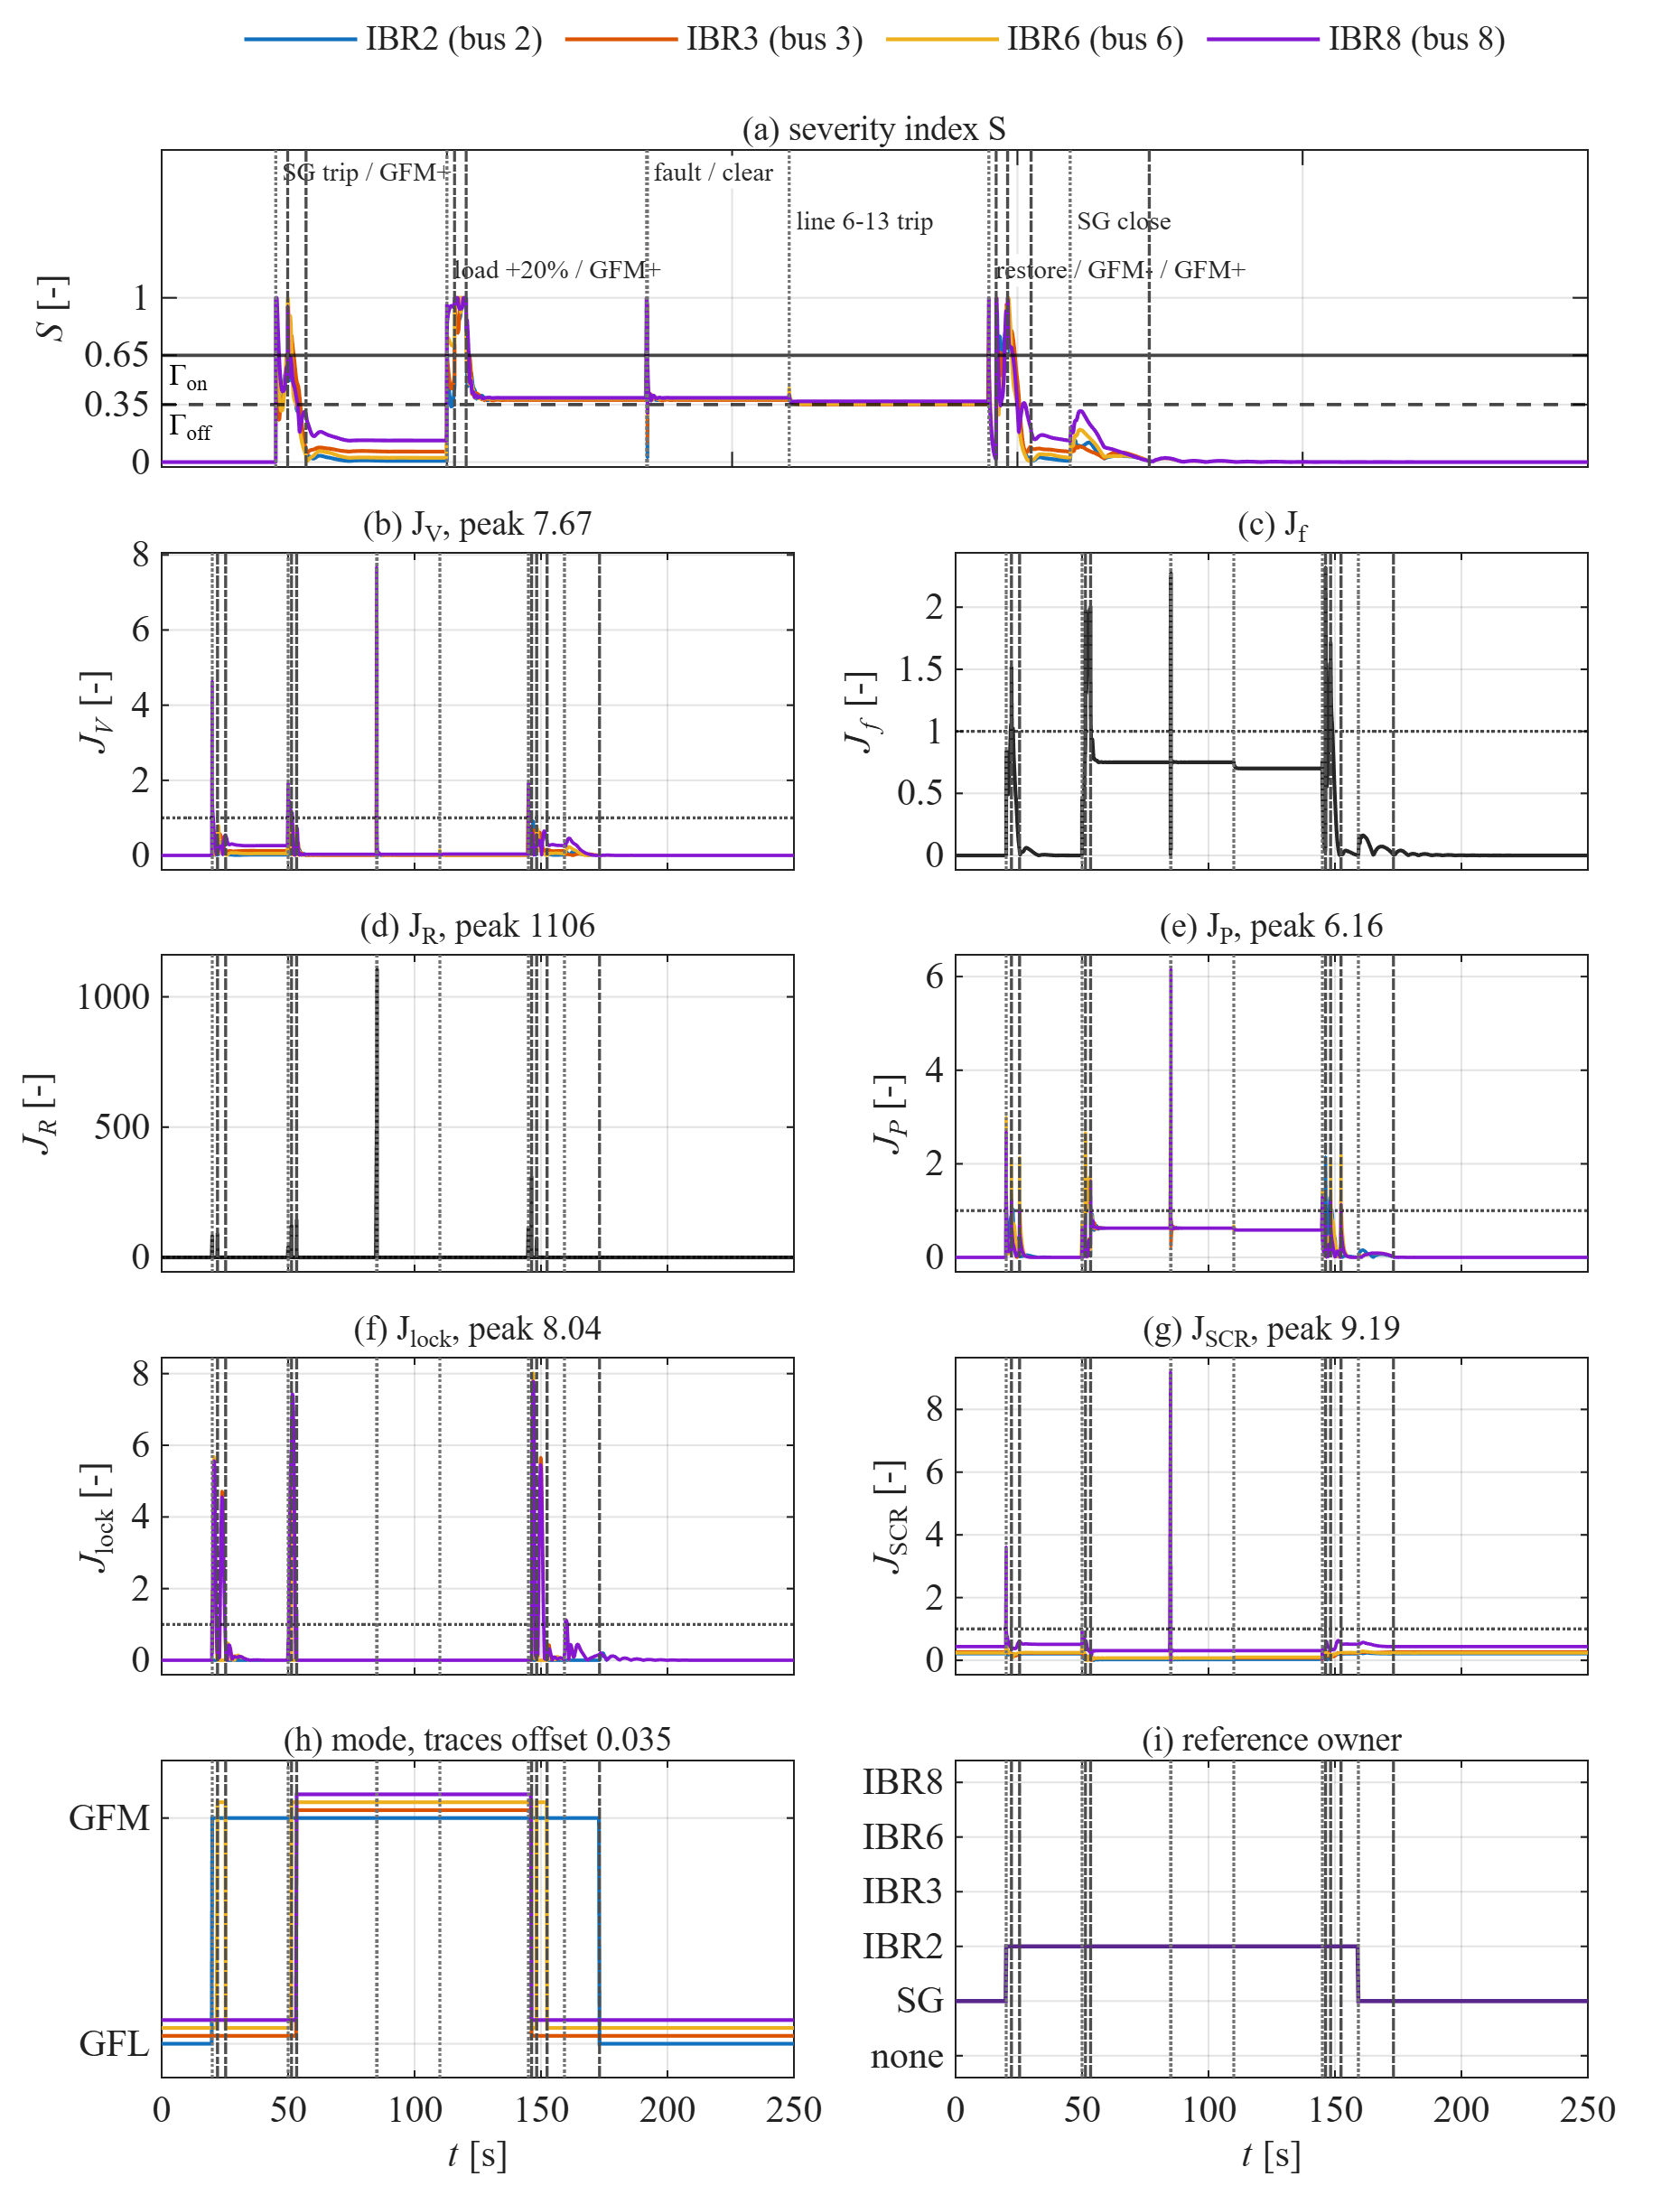
\includegraphics[width=6.20in]{figures/switch_ieee14_decision/decision_indices.png}}
 {\fbox{\parbox{6.0in}{\centering\vspace{3em}\ttfamily decision\_indices.png\\[4pt]
   \normalfont รอการสร้างรูปใหม่
   (รัน \texttt{generate\_ieee14\_switch\_evidence}).\vspace{3em}}}}
\caption{หลักฐานการตัดสินใจสลับโหมด ทุกแผงใช้แกนเวลาเดียวกันและเส้นเหตุการณ์ชุดเดียวกัน
(a) ดัชนีความรุนแรง $S=\sat_{[0,1]}(0.5J_V+0.5J_f)$ พร้อมเส้นเกณฑ์
$\Gamma_{\mathrm{on}}=0.65$ และ $\Gamma_{\mathrm{off}}=0.35$
(b) $J_V$ (c) $J_f$ ของระบบ (d) $J_R$ ของระบบ (e) $J_P$ (f) $J_{\mathrm{lock}}$
(g) $J_{\mathrm{SCR}}$ (h) โหมด GFL/GFM รายตัว (i) เจ้าของมุมอ้างอิง
เส้นจุด: เหตุการณ์รบกวน เส้นจุด--ขีด: คำสั่งของตัวกำกับ
แผง (a)--(c) เป็นตัวตัดสิน แผง (d)--(g) เป็นดัชนีอ้างอิงที่ไม่เข้าเกตใด}
\label{fig:agsi}
\end{figure}

หน้าต่างสองช่วงที่การสลับเกิดขึ้นจริงถูกขยายไว้ในรูปที่~\ref{fig:agsizoom1}
และรูปที่~\ref{fig:agsizoom2} ในสองรูปนี้เส้นทั้งสองตระกูลถูกกำกับชื่อครบ จึงอ่านได้
ว่าค่าดัชนีอยู่ที่เท่าไรในวินาทีที่คำสั่งเกิด

\begin{figure}[H]
\centering
\IfFileExists{figures/switch_ieee14_decision/decision_indices_zoom_island.png}
 {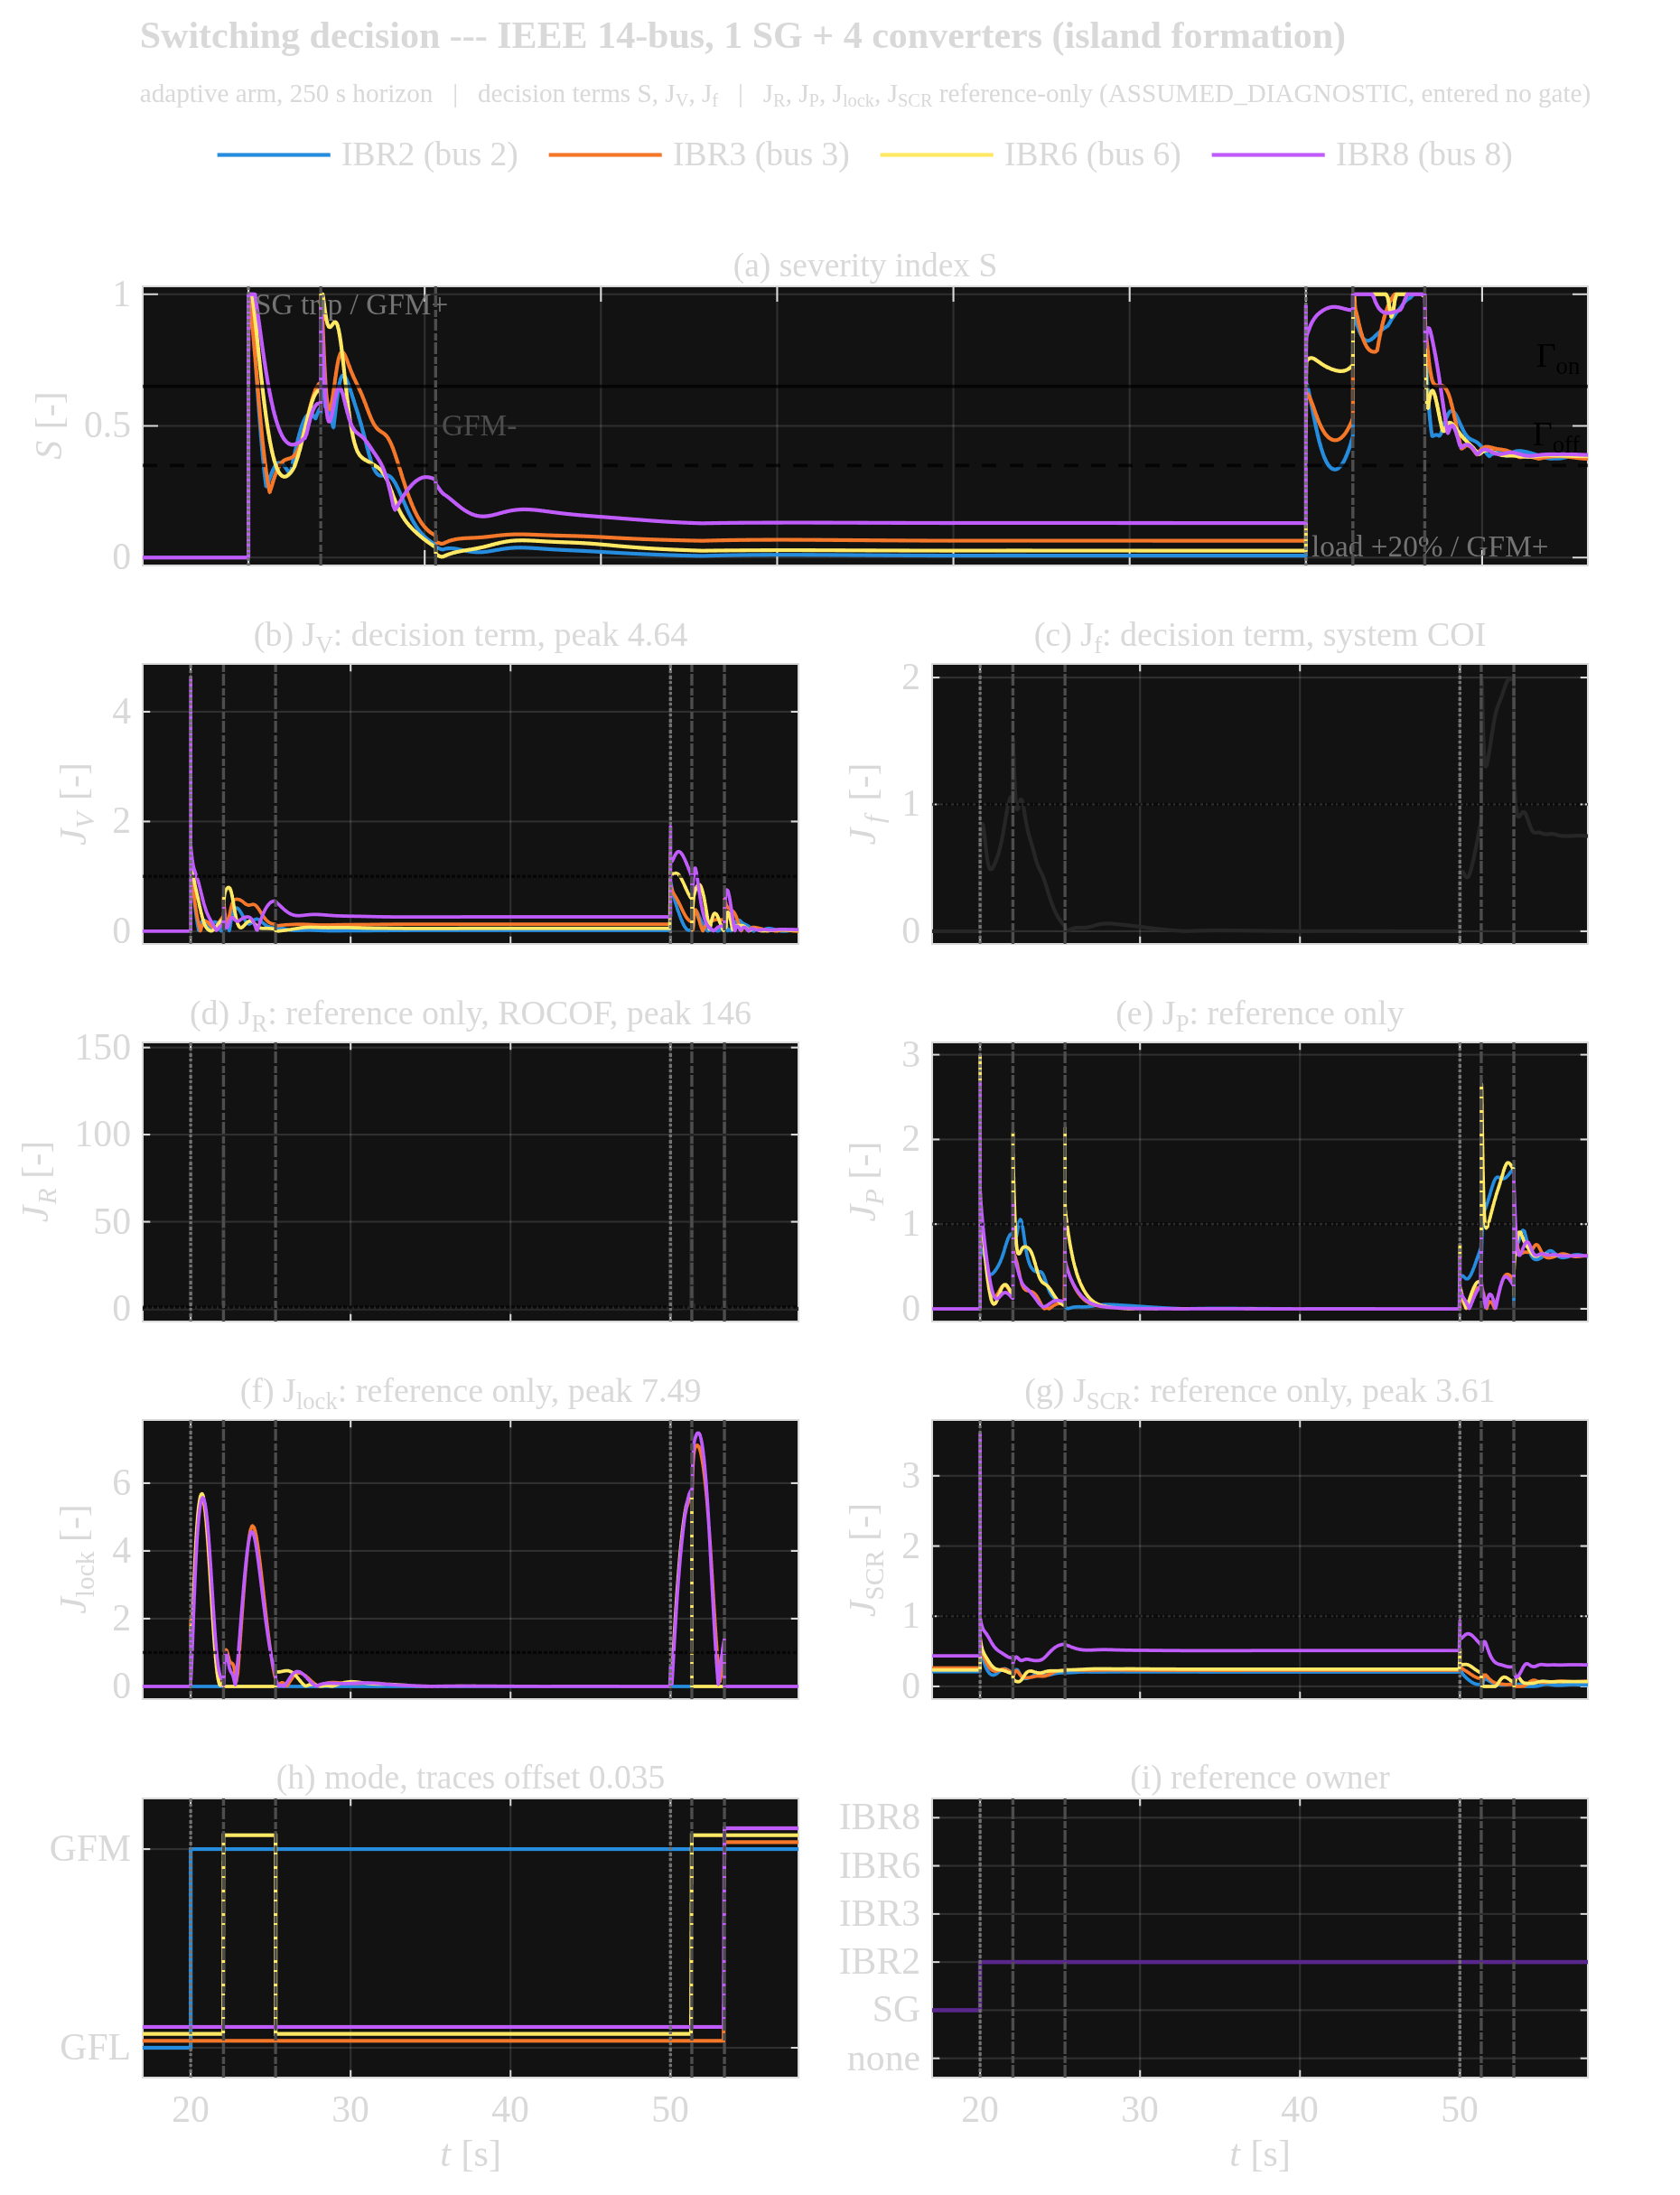
\includegraphics[width=6.20in]{figures/switch_ieee14_decision/decision_indices_zoom_island.png}}
 {\fbox{\parbox{6.0in}{\centering\vspace{3em}\ttfamily
   decision\_indices\_zoom\_island.png\\[4pt]\normalfont
   รอการสร้างรูปใหม่.\vspace{3em}}}}
\caption{ช่วงสร้างเกาะไฟฟ้า $t\in[17,58]\second$ ครอบคลุมการตัด SG การเลื่อนโหมดขึ้น
สองครั้งแรก การปลดหนึ่งครั้ง และโหลดเพิ่มแบบขั้น แผงและเส้นเหมือนรูปที่~\ref{fig:agsi}
ทุกประการ ต่างเพียงช่วงแกนเวลา ไม่มีจุดตัวอย่างใดถูกตัดหรือแก้ค่า}
\label{fig:agsizoom1}
\end{figure}

\begin{figure}[H]
\centering
\IfFileExists{figures/switch_ieee14_decision/decision_indices_zoom_reclose.png}
 {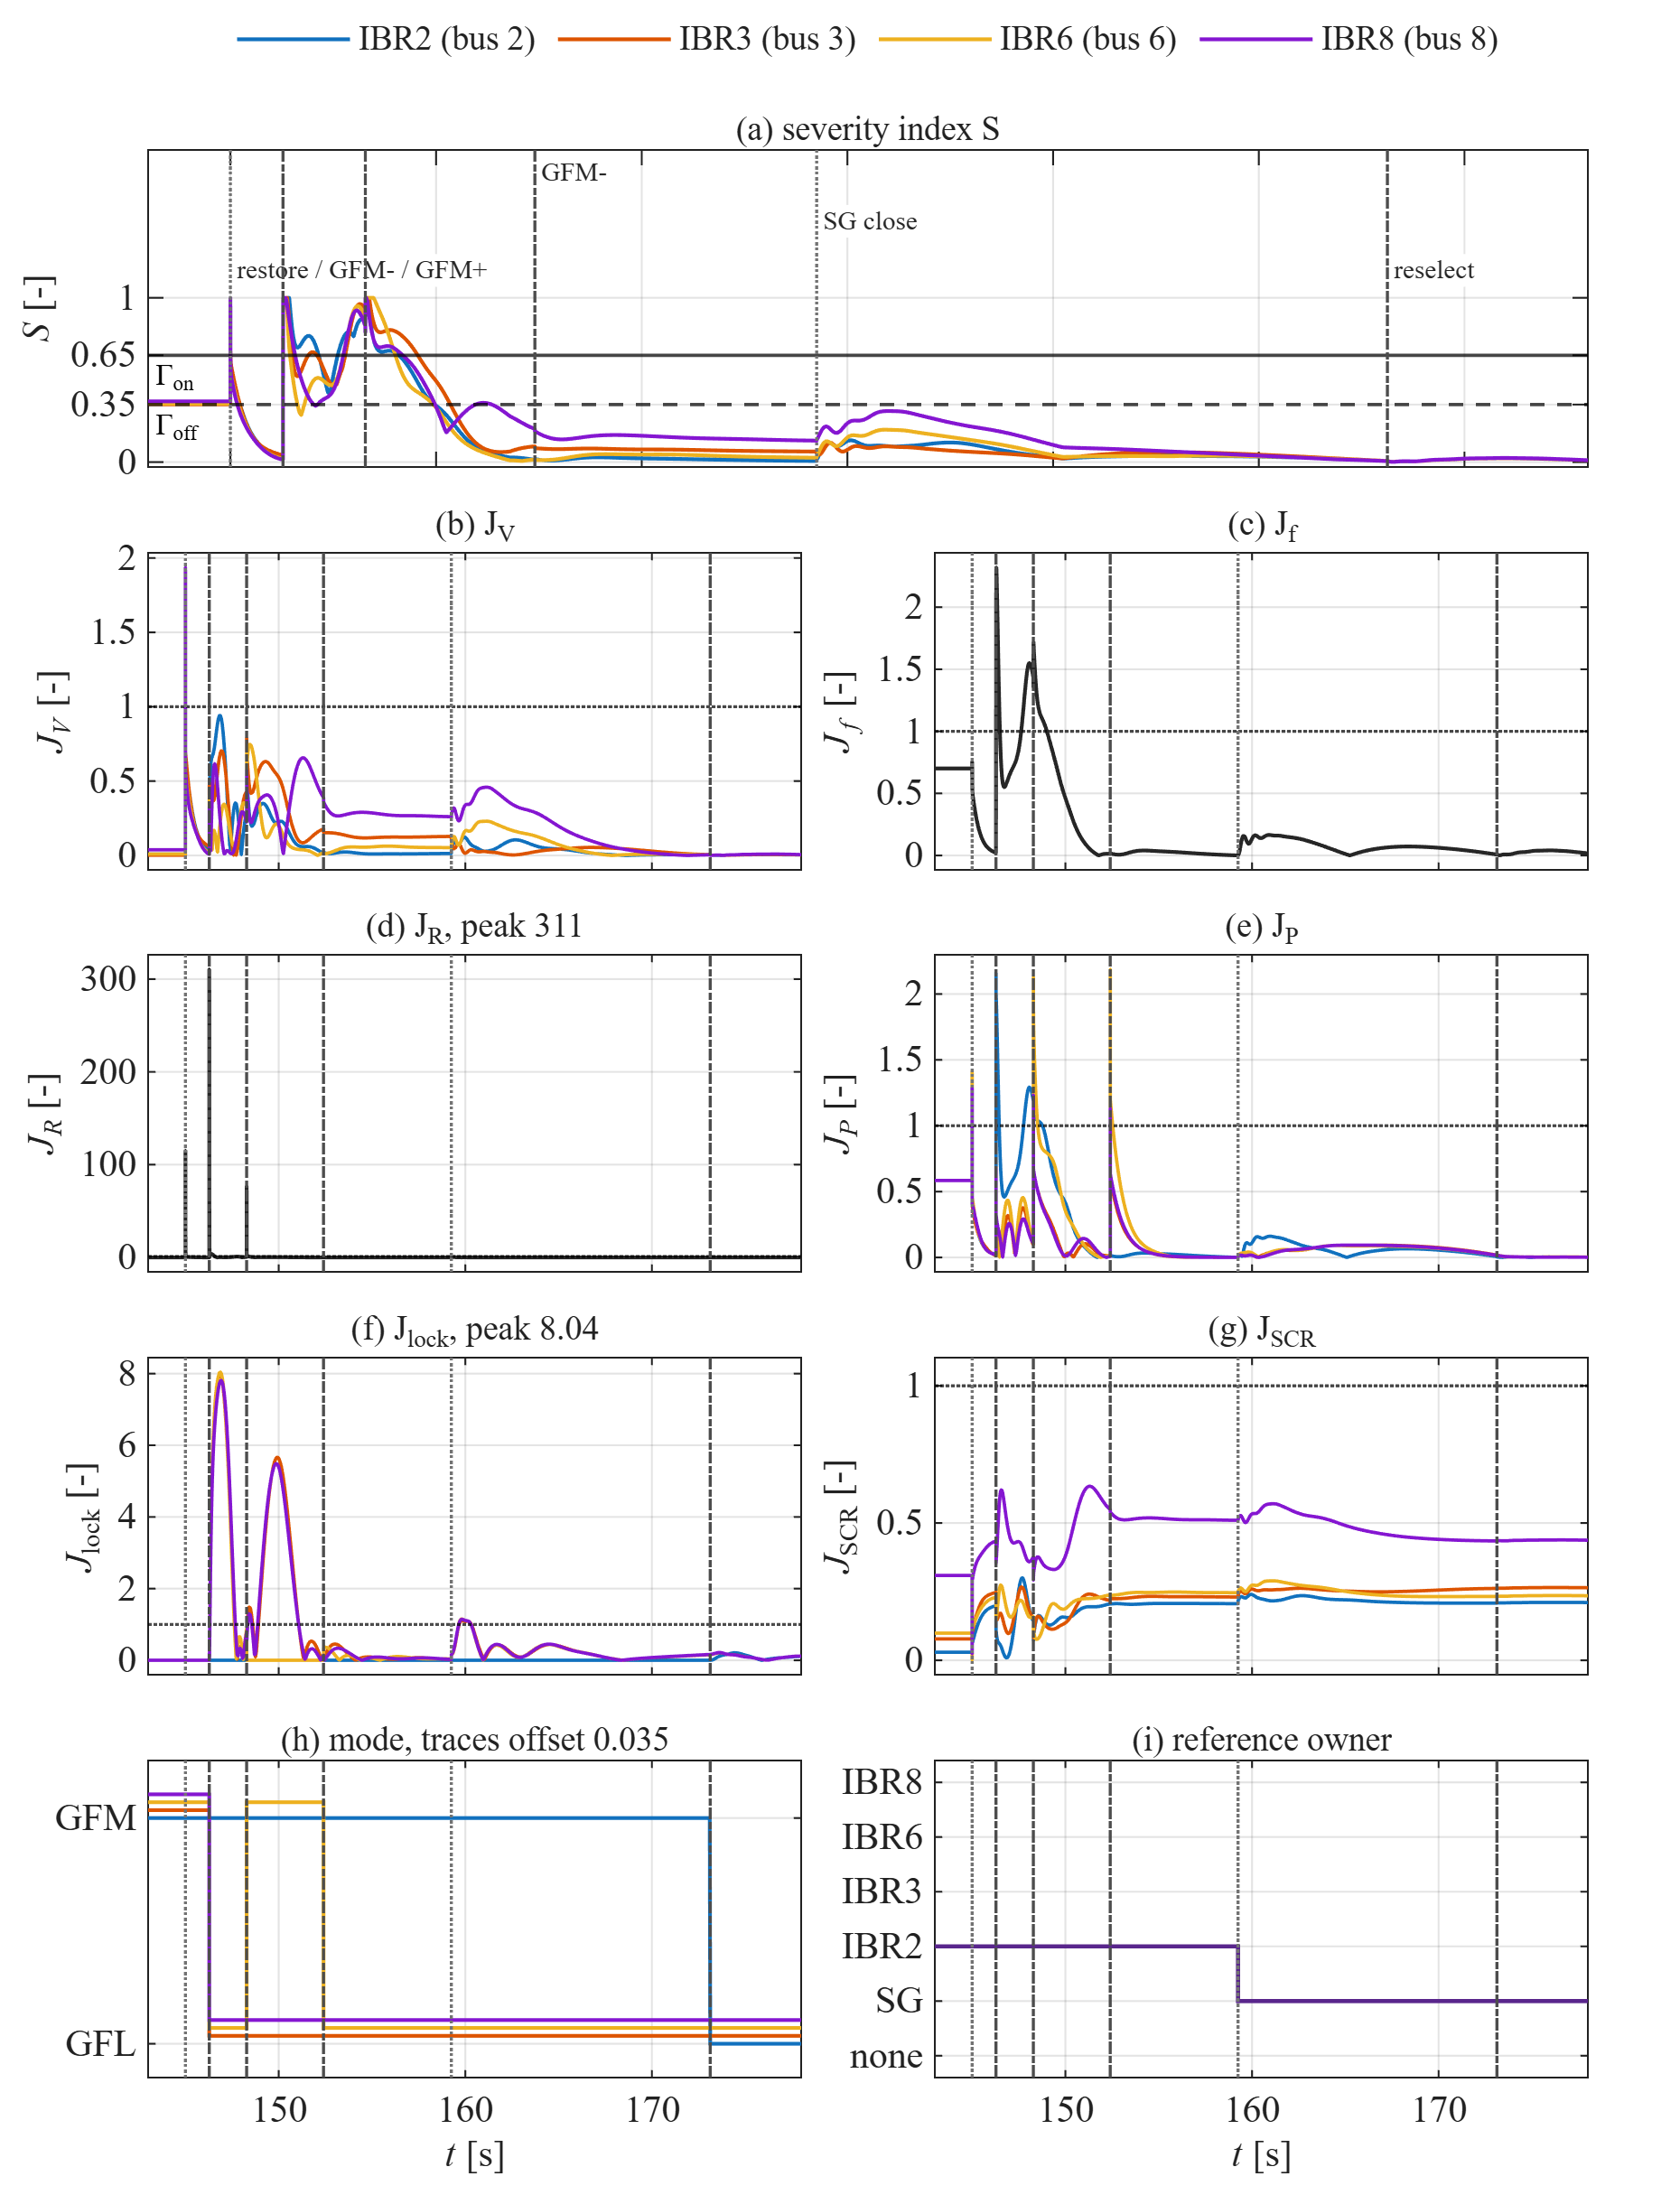
\includegraphics[width=6.20in]{figures/switch_ieee14_decision/decision_indices_zoom_reclose.png}}
 {\fbox{\parbox{6.0in}{\centering\vspace{3em}\ttfamily
   decision\_indices\_zoom\_reclose.png\\[4pt]\normalfont
   รอการสร้างรูปใหม่.\vspace{3em}}}}
\caption{ช่วงต่อกลับและคืนหน้าที่ $t\in[143,178]\second$ เห็นการปลดโหมด การเลื่อนขึ้น
ชดเชยหนึ่งครั้ง การต่อกลับที่ $\NewRunReclose\second$ และการคืนความเป็นเจ้าของมุม
อ้างอิงให้ SG แผงและเส้นเหมือนรูปที่~\ref{fig:agsi} ทุกประการ}
\label{fig:agsizoom2}
\end{figure}

%=============================================================================
\section{เครื่องกำเนิดไฟฟ้าซิงโครนัส: แบบจำลองอันดับหกและการพิสูจน์}\label{sec:sg}
%=============================================================================
SG ในงานนี้เป็นเครื่องอันดับหก (โครงสร้างตาม IEEE~1110 Model~2.2 / GENTPJ แบบ
โรเตอร์กลม) มีเวกเตอร์สเตตและอินพุต
\begin{equation}
  x_{\mathrm{sg}}=[\,\delta,\;\omega,\;E_q',\;E_d',\;E_q'',\;E_d''\,]^{\top},
  \qquad u_{\mathrm{sg}}=[\,T_m,\;E_{fd}\,]^{\top},
  \label{eq:sgstate}
\end{equation}
โดย $\delta$ คือมุมโรเตอร์ $\omega$ คือความเบี่ยงเบนความเร็วต่อหน่วย (สลิป)
$E_q',E_d'$ คือแรงเคลื่อนไฟฟ้าชั่วครู่ และ $E_q'',E_d''$ คือแรงเคลื่อนไฟฟ้าชั่วครู่
ย่อย อินพุตควบคุมสองตัวคือ $T_m$ (ทอร์กทางกล) และ $E_{fd}$ (แรงดันกระตุ้นสนาม)
ถูกตรึงไว้ที่ค่าที่ได้จากการแก้จุดสมดุลของเครือข่ายผสม และไม่ถูกแก้ใหม่ทุกขั้นเวลา
เหตุที่ตรึงได้คือในสถานการณ์นี้ไม่มีการจำลอง governor/AVR แบบวงปิดของ SG เอง
สิ่งที่สนใจคือพฤติกรรมของเครื่องเมื่อถูกตัดออกและต่อกลับ ไม่ใช่การตอบสนองของระบบ
ควบคุมเชื้อเพลิงและการกระตุ้น

\subsection{การอนุมานทีละอันดับ}
สมการของเครื่องขณะเชื่อมต่อเครือข่าย เขียนทีละพจน์ตรงตามที่โค้ดคำนวณ คือ
\begin{align}
  \dot\delta            &= \omega_0\,\omega, \label{eq:sg1}\\
  2H\,\dot\omega        &= T_m - T_e - D\,\omega, \label{eq:sg2}\\
  T_{d0}'\,\dot{E}_q'   &= E_{fd} + c_d E_q'' - d_d E_q', \label{eq:sg3}\\
  T_{q0}'\,\dot{E}_d'   &= c_q E_d'' - d_q E_d', \label{eq:sg4}\\
  T_{d0}''\,\dot{E}_q''  &= E_q' - E_q'' - (X_d'-X_d'')\,I_d, \label{eq:sg5}\\
  T_{q0}''\,\dot{E}_d''  &= E_d' - E_d'' + (X_q'-X_q'')\,I_q, \label{eq:sg6}
\end{align}
โดย $\omega_0=2\pi f_0$ ทอร์กไฟฟ้าช่องอากาศที่ปิดสมการการแกว่ง~\eqref{eq:sg2} คือ
\begin{equation}
  T_e = V_d I_d + V_q I_q + R_a\,(I_d^2+I_q^2), \label{eq:sgte}
\end{equation}
และสัมประสิทธิ์การประกบฟลักซ์ทั้งสี่นิยามจากบันไดค่ารีแอกแตนซ์ว่า
\begin{equation}
  c_d=\frac{X_d-X_d'}{X_d'-X_d''},\quad
  d_d=\frac{X_d-X_d''}{X_d'-X_d''},\quad
  c_q=\frac{X_q-X_q'}{X_q'-X_q''},\quad
  d_q=\frac{X_q-X_q''}{X_q'-X_q''}.
  \label{eq:cddd}
\end{equation}

\emph{แต่ละอันดับคืออะไร} สมการ~\eqref{eq:sg1}--\eqref{eq:sg2} คือพลวัตทางกล
(อันดับสอง) ได้แก่มุมและความเร็ว โดย~\eqref{eq:sg2} คือสมการการแกว่ง (swing
equation) ที่กล่าวว่าอัตราการเปลี่ยนความเร็วเป็นสัดส่วนกับส่วนต่างระหว่างทอร์กทางกล
ที่ป้อนเข้ากับทอร์กไฟฟ้าที่ถูกดึงออก หักด้วยการหน่วง $D\omega$
สมการ~\eqref{eq:sg3}--\eqref{eq:sg4} คือฟลักซ์ชั่วครู่ (ขดลวดสนามโรเตอร์และแดมเปอร์
แกน q) ซึ่งเปลี่ยนบนค่าคงที่เวลาช้า $T_{d0}',T_{q0}'$ ส่วน
สมการ~\eqref{eq:sg5}--\eqref{eq:sg6} คือฟลักซ์ชั่วครู่ย่อย (ขดลวดแดมเปอร์) ที่
เปลี่ยนบนค่าคงที่เวลาเร็ว $T_{d0}'',T_{q0}''$ พจน์ปฏิกิริยาอาร์เมเจอร์
$-(X_d'-X_d'')I_d$ และ $+(X_q'-X_q'')I_q$ คือสิ่งที่ประกบฟลักซ์เร็วเข้ากับกระแส
สเตเตอร์ พูดอย่างรวบยอดคือ แบบจำลองนี้แยกพลวัตออกเป็นสามช่วงเวลา: กลไกทางกลที่ช้า
ที่สุด ฟลักซ์สนามที่เร็วกว่า และฟลักซ์แดมเปอร์ที่เร็วที่สุด

\emph{หลักยึดของการพิสูจน์ --- เอกลักษณ์ $d-c=1$}
จาก~\eqref{eq:cddd} จะได้
\begin{equation}
  d_d-c_d=\frac{(X_d-X_d'')-(X_d-X_d')}{X_d'-X_d''}
         =\frac{X_d'-X_d''}{X_d'-X_d''}=1,
  \qquad\text{และในทำนองเดียวกัน } d_q-c_q=1.
  \label{eq:identity}
\end{equation}
พิจารณาสภาวะคงตัวขณะเปิดวงจร ($I_d=I_q=0$, $\dot x=0$) จาก~\eqref{eq:sg5} ได้
$E_q''=E_q'$ แทนกลับใน~\eqref{eq:sg3} จะได้
\begin{equation}
  0=E_{fd}+c_d E_q'-d_d E_q'=E_{fd}-(d_d-c_d)E_q'=E_{fd}-E_q'
  \;\Longrightarrow\; E_q'=E_{fd}.
\end{equation}
ดังนั้นเอกลักษณ์~\eqref{eq:identity} คือสิ่งที่ทำให้แรงเคลื่อนไฟฟ้าสนามขณะเปิดวงจร
เท่ากับแรงดันกระตุ้นที่ป้อนเข้าพอดี ซึ่งเป็นการตรวจความสอดคล้องมาตรฐานของการ
พารามิเตอร์ฟลักซ์แบบนี้ และเป็นเหตุผลที่สัมประสิทธิ์ต้องเขียนเป็น\emph{อัตราส่วน}
ตาม~\eqref{eq:cddd} ไม่ใช่ค่าคงที่อิสระที่ปรับได้ตามใจ การอนุมานเดียวกันบนแกน q
ให้ $E_d'=0$ ขณะเปิดวงจร เพราะไม่มีแหล่งกระตุ้นที่เทียบเท่า $E_{fd}$ บนแกนนั้น
ประโยชน์เชิงปฏิบัติของเอกลักษณ์นี้คือ ใช้เป็นการตรวจสอบข้อผิดพลาดของการถอดสมการได้
ทันทีโดยไม่ต้องรันการจำลอง: หากโค้ดใดให้ $d_d-c_d\ne1$ แสดงว่าถอดสมการผิด

\subsection{อินเทอร์เฟซพีชคณิตของสเตเตอร์}
กระแสสเตเตอร์\emph{ไม่ได้}ถูกย้อนคำนวณจากกำลัง แต่ถูกแก้จากแรงเคลื่อนไฟฟ้าชั่วครู่
ย่อยที่อยู่หลังรีแอกแตนซ์ชั่วครู่ย่อย โดยฉายแรงดันที่ขั้วเชิงซ้อน $V$ ลงบนกรอบ $dq$
ของเครื่อง ($V_d,V_q$) แล้วกำหนด $r_d=V_d-E_d''$, $r_q=V_q-E_q''$ จะได้
\begin{equation}
  \det=X_d''X_q''+R_a^2,\qquad
  I_d=\frac{-R_a r_d - X_q'' r_q}{\det},\qquad
  I_q=\frac{X_d'' r_d - R_a r_q}{\det},
  \label{eq:stator}
\end{equation}
ซึ่งเป็นอินเวอร์สที่แน่นอนของความสัมพันธ์สเตเตอร์ชั่วครู่ย่อย
$V_d=E_d''-R_a I_d+X_q'' I_q$ และ $V_q=E_q''-R_a I_q-X_d'' I_d$ ทอร์ก
ไฟฟ้า~\eqref{eq:sgte} ใช้ $I_d,I_q$ ชุดเดียวกันนี้

\emph{ทำไมต้องทำแบบนี้} หากย้อนคำนวณกระแสจากกำลังที่ต้องการ ($I=S^{*}/V^{*}$)
กระแสจะกลายเป็นตัวแปรที่ถูกกำหนดจากภายนอกและตัดพลวัตของฟลักซ์ออกจากวงจร ผลคือ
เครื่องจะไม่แสดงพฤติกรรมชั่วครู่ย่อยเลย และค่ากระแสตอนเกิดฟอลต์จะไม่สะท้อนความจริง
การแก้จาก~\eqref{eq:stator} รักษาให้กระแสเป็น\emph{ผลลัพธ์}ของสเตตฟลักซ์และแรงดัน
ที่ขั้วเสมอ ซึ่งจำเป็นต่อการตรวจสอบการต่อกลับของเบรกเกอร์

\subsection{ลิมิตเอกฐานที่ตรึงสเตต $E_d'$}\label{sec:frozen}
สำหรับข้อมูลเครื่องที่ใช้ในงานนี้ ค่าคงที่เวลาขณะเปิดวงจรของฟลักซ์ชั่วครู่แกน q
ถูกกำหนดไว้ที่ลิมิตเอกฐาน $T_{q0}'=0$ (เป็นกรณีโรเตอร์กลมที่ผ่านการตรวจสอบแล้ว)
เมื่อเป็นเช่นนี้ สมการ~\eqref{eq:sg4} ไม่ใช่สมการเชิงอนุพันธ์อีกต่อไป แต่ลดรูปเป็น
ข้อบังคับเชิงพีชคณิต
\begin{equation}
  0 = c_q E_d'' - d_q E_d'.
\end{equation}
สำหรับเครื่องนี้ $c_q=0$ และ $d_q=1$ ดังนั้น $E_d'\equiv 0$ โค้ดตรวจพบเงื่อนไข
$T_{q0}'=0$ แบบตรงตัว และ\emph{ถอด} $E_d'$ (สเตตดัชนีที่ 4) ออกจากชุดที่ถูก
อินทิเกรต โดยคงค่าไว้ที่ค่าพีชคณิต $0$ ผลคือ SG ส่งสเตตพลวัตเข้าระบบรวม
\textbf{ห้า} ตัว คือ $[\delta,\omega,E_q',E_q'',E_d'']$ ไม่ใช่หกตัว นี่คือลิมิต
เอกฐานแบบ \textsf{SOURCE\_DEFINED} ไม่ใช่ความสะดวกเชิงตัวเลข เพราะเป็นการลดรูป
$T_{q0}'\to0$ ของสมการชุดเดิม การแยกแยะนี้สำคัญ: ถ้าปล่อยให้ $E_d'$ ถูกอินทิเกรต
ต่อโดยหารด้วย $T_{q0}'=0$ จะเกิดการหารด้วยศูนย์ และถ้า ``แก้'' ด้วยการใส่ค่า
$T_{q0}'$ เล็ก ๆ แทน จะกลายเป็นการเปลี่ยนพารามิเตอร์ของเครื่องเพื่อความสะดวกเชิง
ตัวเลข ซึ่งขัดกับข้อกำหนดความสมบูรณ์เชิงตัวเลขของโครงการ

\subsection{การไหลตามแรงเฉื่อยเมื่อเบรกเกอร์เปิด}
เมื่อเบรกเกอร์ของ SG เปิดที่ $t=20$~s เครื่องจักร\emph{ไม่ได้}หายไปจากเวกเตอร์สเตต
สิ่งที่เกิดขึ้นคือกระแสอัดเข้าเครือข่ายกลายเป็นศูนย์ ($I_d=I_q=0$ จึงได้ $T_e=0$)
และฟลักซ์สลายตัวบนกิ่งเปิดวงจรของ~\eqref{eq:sg3}--\eqref{eq:sg6} (พจน์ปฏิกิริยา
อาร์เมเจอร์หายไปเพราะ $I_d=I_q=0$) ขณะที่สมการการแกว่ง~\eqref{eq:sg1}--\eqref{eq:sg2}
ไหลต่อไปตามแรงเฉื่อยบนทอร์กทางกลที่ถูกตรึงไว้ แผนที่ที่รายงานว่า SG อินทิเกรตสเตต
กี่ตัวนั้นไม่ขึ้นกับบริบท: มันคืนค่า $[\,1,2,3,5,6\,]$ ทั้งกรณีเบรกเกอร์ปิดและเปิด
ผลที่ตามมาคือการสูญเสีย SG slack \emph{ไม่ได้}เปลี่ยนจำนวนสเตตของ SG เอง มิติของ
ระบบรวมเปลี่ยนเพราะ IBR สลับโหมดเท่านั้น (หัวข้อ~\ref{sec:ibr})

\emph{เหตุใดต้องเก็บ SG ไว้ในเวกเตอร์สเตต} เพราะการต่อกลับในช่วง 6 ต้องอาศัยมุมและ
ความเร็วของโรเตอร์ที่ผ่านการไหลตามแรงเฉื่อยมา ถ้าลบเครื่องออกจากระบบตอนถูกตัด เมื่อ
จะต่อกลับก็จะไม่มีสถานะภายในให้เทียบเฟส และการต่อกลับจะกลายเป็นการสร้างเครื่องใหม่
ที่มุมใดก็ได้ ซึ่งไม่สอดคล้องกับกายภาพของการซิงโครไนซ์

%=============================================================================
\section{อินเวอร์เตอร์: แบบจำลองสองโหมดขนาด 16 สเตต}\label{sec:ibr}
%=============================================================================
IBR แต่ละตัวเป็น\emph{อุปกรณ์ชิ้นเดียว}ที่สามารถแสดงตัวควบคุมได้สองแบบบนภาคกำลัง
ร่วมชุดเดียวกัน เวกเตอร์สเตตเต็มมีขนาดคงที่ 16 ตัว
\begin{equation}
  x_{\mathrm{IBR}}
   =\bigl[\underbrace{i_d,\,i_q,\,V_{dc}}_{x_{\mathrm{pl}}\;(3)}\;\big|\;
          \underbrace{x_{\mathrm{GFL}}\;(6)}_{\text{ดัชนี }4\text{--}9}\;\big|\;
          \underbrace{x_{\mathrm{GFM}}\;(7)}_{\text{ดัชนี }10\text{--}16}\bigr]^{\top}
   \in\mathbb{R}^{16},
   \label{eq:ibrstate}
\end{equation}
ซึ่งเรียงตามลำดับจริงในโค้ด (ABI) โดยบล็อกตัวควบคุมเขียนแยกกันดังนี้
\begin{align}
  x_{\mathrm{GFL}}&=[\,\delta_{\mathrm{PLL}},\,\xi_{\mathrm{PLL}},\,\xi_P,\,\xi_Q,
      \,\xi_{Id},\,\xi_{Iq}\,],\\
  x_{\mathrm{GFM}}&=[\,\delta_{\mathrm{VSG}},\,\omega_{\mathrm{VSG}},\,E,
      \,\xi_{Vd},\,\xi_{Vq},\,\xi_{Id},\,\xi_{Iq}\,].
\end{align}
ณ ขณะใดขณะหนึ่ง มีเพียง\emph{ภาพฉาย} (projection) ของ~\eqref{eq:ibrstate} เท่านั้น
ที่ถูกอินทิเกรต แผนที่ดัชนีที่แอ็กทีฟคืนค่า
\begin{equation}
  \mathcal{A}_{\mathrm{GFL}}=\{1{:}9\},\qquad
  \mathcal{A}_{\mathrm{GFM}}=\{1{:}3,\,10{:}16\},\qquad
  \mathcal{A}_{\mathrm{tripped}}=\varnothing,
  \label{eq:ibractive}
\end{equation}
กล่าวคือ 9 สเตตแอ็กทีฟในโหมด GFL, 10 สเตตในโหมด GFM และไม่มีสเตตใดแอ็กทีฟเมื่อ
อุปกรณ์ถูกตัดออก บล็อกภาคกำลังร่วมแอ็กทีฟตลอดเวลา ส่วนบล็อกตัวควบคุมสองชุดใช้งาน
แบบไม่ทับซ้อนกัน (mutually exclusive)

ตารางที่~\ref{tab:ibrstates} แจกแจงทั้ง 16 สเตตตามลำดับดัชนีจริง พร้อมระบุว่าสเตต
ใดแอ็กทีฟในโหมดใด สัญลักษณ์ $\bullet$ หมายถึงถูกอินทิเกรต และ $\circ$ หมายถึงถูก
ตรึงค่าไว้ (frozen) ประเด็นที่ควรชี้ให้เห็นตอนนำเสนอคือ PLL ปรากฏ\emph{เฉพาะ}ใน
บล็อก GFL และไม่มีอยู่ในบล็อก GFM เลย ขณะที่บล็อก GFM มีสมการการแกว่งเสมือนแทน

\begin{table}[H]
\centering\footnotesize
\caption{แจกแจงสเตตทั้ง 16 ตัวของ IBR ตามลำดับดัชนีในโค้ด: ดัชนี 1--3 คือภาคกำลัง
ร่วมที่แอ็กทีฟทั้งสองโหมด ดัชนี 4--9 คือตัวควบคุม GFL และดัชนี 10--16 คือตัวควบคุม
GFM}
\label{tab:ibrstates}
\begin{tabular}{@{}c l l c c@{}}
\toprule
\# & สเตต & ความหมาย & GFL & GFM \\ \midrule
\multicolumn{5}{@{}l}{\textit{ภาคกำลังร่วม (แอ็กทีฟทั้งสองโหมด)}}\\
1 & $i_d$ & กระแสตัวกรองแกน d & $\bullet$ & $\bullet$ \\
2 & $i_q$ & กระแสตัวกรองแกน q & $\bullet$ & $\bullet$ \\
3 & $V_{dc}$ & แรงดันบัส DC & $\bullet$ & $\bullet$ \\
\midrule
\multicolumn{5}{@{}l}{\textit{ตัวควบคุม GFL (ตรึงเมื่ออยู่ในโหมด GFM)}}\\
4 & $\delta_{\mathrm{PLL}}$ & มุมของ PLL & $\bullet$ & $\circ$ \\
5 & $\xi_{\mathrm{PLL}}$ & ตัวอินทิเกรตของ PLL & $\bullet$ & $\circ$ \\
6 & $\xi_{P}$ & ตัวอินทิเกรตวงรอบกำลังจริง & $\bullet$ & $\circ$ \\
7 & $\xi_{Q}$ & ตัวอินทิเกรตวงรอบกำลังรีแอกทีฟ & $\bullet$ & $\circ$ \\
8 & $\xi_{Id}$ & ตัวอินทิเกรตกระแสชั้นในแกน d & $\bullet$ & $\circ$ \\
9 & $\xi_{Iq}$ & ตัวอินทิเกรตกระแสชั้นในแกน q & $\bullet$ & $\circ$ \\
\midrule
\multicolumn{5}{@{}l}{\textit{ตัวควบคุม GFM (ตรึงเมื่ออยู่ในโหมด GFL)}}\\
10 & $\delta_{\mathrm{VSG}}$ & มุมของเครื่องซิงโครนัสเสมือน & $\circ$ & $\bullet$ \\
11 & $\omega_{\mathrm{VSG}}$ & ความถี่ของเครื่องซิงโครนัสเสมือน & $\circ$ & $\bullet$ \\
12 & $E$ & แอมพลิจูดแรงดันที่วงรอบ $Q$--$V$ สร้าง & $\circ$ & $\bullet$ \\
13 & $\xi_{Vd}$ & ตัวอินทิเกรตวงรอบแรงดันแกน d & $\circ$ & $\bullet$ \\
14 & $\xi_{Vq}$ & ตัวอินทิเกรตวงรอบแรงดันแกน q & $\circ$ & $\bullet$ \\
15 & $\xi_{Id}$ & ตัวอินทิเกรตกระแสชั้นในแกน d & $\circ$ & $\bullet$ \\
16 & $\xi_{Iq}$ & ตัวอินทิเกรตกระแสชั้นในแกน q & $\circ$ & $\bullet$ \\
\midrule
\multicolumn{3}{@{}l}{\textit{จำนวนสเตตแอ็กทีฟรวม}} & \textit{9} & \textit{10} \\
\bottomrule
\end{tabular}
\end{table}

\subsection{สเตตความหน่วงคำสั่งที่ถูกลดออก}\label{sec:ibr-reduction}
แผนภาพบล็อกของแหล่งอ้างอิงมีความหน่วงของตัวขับอันดับหนึ่งหนึ่งตัวต่อหนึ่งแกน
$T_d\,\dot V_{\mathrm{del}}=v_{\mathrm{cmd}}-V_{\mathrm{del}}$ ซึ่งค่าคงตัวเวลาทาง
กายภาพของมันคือความหน่วงของคอนเวอร์เตอร์เชิงเลข $T_d=1.5/f_{\mathrm{sw}}\approx0.3$~ms
ที่ $f_{\mathrm{sw}}=5$~kHz ค่านี้เล็กกว่าขั้นเวลาแบบเฟเซอร์ที่ใช้ในงานนี้มากกว่าสอง
อันดับของสิบ ดังนั้นตามทฤษฎีการก่อกวนเอกฐาน (singular perturbation) ความหน่วงที่เร็ว
กว่ามากจะยุบลงบนแมนิโฟลด์ช้าของตัวเอง $V_{\mathrm{del}}=v_{\mathrm{cmd}}$ สเตตความ
หน่วงสองตัวต่อหนึ่งกิ่งจึงถูกกำจัดออกเชิงพีชคณิต และสมการกระแสของตัวกรองใช้คำสั่ง
แรงดัน $v_{cd},v_{cq}$ โดยตรง

นี่คือการลดอันดับแบบจำลองมาตรฐานซึ่งไม่เปลี่ยนทั้งจุดสมดุลและพลวัตของสเตตที่คงไว้
และยังกำจัดโพลที่อยู่ราว $530$~Hz ซึ่งแบบจำลองเครือข่ายแบบเฟเซอร์ RMS ไม่สามารถ
แทนได้อยู่แล้ว การลดอันดับนี้ทำให้ซูเปอร์เซ็ตสองโหมดลดจาก $20$ เหลือ $16$ สเตต
ตาม~\eqref{eq:ibrstate} และทำให้แต่ละกิ่งเดี่ยวลดจาก $12$ เหลือ $10$ สเตต
การลดอันดับจัดเป็น \textsf{PROJECT\_DERIVED} และเป็นการตัดสินของเจ้าของงาน
ดูบันทึกข้อบกพร่อง \textsf{TD-2026-08-12-01}

\emph{ข้อความที่ต้องระบุตามจริง} รายงานฉบับก่อนหน้านี้พิมพ์ผังสเตตขนาด $20$ ตัว
ก่อนการลดอันดับ ซึ่งเป็นผังที่แบบจำลองที่รันจริง\emph{ไม่มี}อีกแล้ว

\paragraph{ตัวดำเนินการสองตัวที่ใช้ซ้ำในทั้งสองโหมด}
$\Pi_I(a,b;I_{\max})$ คือตัวจำกัดกระแสแบบ\emph{วงกลม}: ถ้า $r=\sqrt{a^2+b^2}>I_{\max}$
จะสเกลคู่อันดับ $(a,b)\mapsto(a,b)\,I_{\max}/r$ ถ้าไม่เกินก็คืนค่าเดิม ส่วนที่ถูก
ตัดออกเรียกว่าเรซิดวลของตัวจำกัด $r_i=(a,b)-\Pi_I(a,b)$ เหตุที่ต้องจำกัดเป็นวงกลม
ไม่ใช่จำกัดแยกแกน เพราะขนาดกระแสจริงของอินเวอร์เตอร์คือขนาดเวกเตอร์รวม การจำกัดแยก
แกนจะยอมให้ขนาดรวมทะลุพิกัดได้ถึง $\sqrt2$ เท่า

$\mathcal{H}(e,\gamma,r_i,\text{sat})$ คือตัวอินทิเกรตแบบมีเงื่อนไขกันการอิ่มตัว
สะสม: คืนค่า $0$ เมื่อค่าอ้างอิงถูกตัด\emph{และ}ความผิดพลาดกำลังจะสะสมต่อไปในทิศ
เดิม (เงื่อนไข $\text{sat}$ เป็นจริง และ $\gamma\,e\,r_i>0$) และคืนค่า $e$ ในกรณี
อื่น กลไกนี้ป้องกันอาการที่ตัวอินทิเกรตสะสมค่าไว้ระหว่างที่เอาต์พุตถูกตัด แล้วทำให้
ระบบตอบสนองช้าผิดปกติเมื่อออกจากการอิ่มตัว

กระแสอัดเข้าเครือข่ายและกำลังที่ขั้วนิยามว่า
$I=(i_d+\mathrm{j}i_q)e^{\mathrm{j}\theta}/\kappa$, $S=V\overline{I}$,
$P_{\mathrm{inv}}=\kappa\Re S$, $Q_{\mathrm{inv}}=\kappa\Im S$ โดย
$\kappa=S_{\mathrm{base}}/M_{\mathrm{base}}$ และ
$(v_d,v_q)=\Re,\Im\,(Ve^{-\mathrm{j}\theta})$ การใช้ $\kappa$ อย่างสม่ำเสมอทั้ง
ในกระแสและกำลังเป็นสิ่งจำเป็น มิฉะนั้นฐานต่อหน่วยของกระแส กำลัง และเกนของตัวควบคุม
จะไม่สอดคล้องกัน

\subsection{ภาคกำลังร่วม (สเตต 1--3)}
พลวัตกระแสของตัวกรองแบบ $L$ และบัส DC ใช้ร่วมกันทั้งสองโหมดและแอ็กทีฟตลอดเวลา
เขียนหนึ่งสเตตต่อหนึ่งบรรทัดตามลำดับดัชนี
\begin{align}
  \tfrac{L}{\omega_b}\,\dot{i}_d &= v_{cd}-v_d-R\,i_d+\omega L\,i_q,
    &&\text{(1) กระแสตัวกรองแกน $d$}\\
  \tfrac{L}{\omega_b}\,\dot{i}_q &= v_{cq}-v_q-R\,i_q-\omega L\,i_d,
    &&\text{(2) กระแสตัวกรองแกน $q$}\\
  \dot{V}_{dc} &= \tfrac{1}{C}\!\left[\tfrac{E_{dc}-V_{dc}}{R_{dc}}-\frac{P_{ac}}{V_{dc}}-\frac{\max(0,\,V_{dc}-V_{dc}^{\max})}{R_{ch}}\right],
    &&\text{(3) แรงดันบัส DC}
\end{align}
โดย $R=R_f$, $L=L_f$, $C=C_{dc}$, $\omega_b=2\pi f_b$ และ $v_{cd},v_{cq}$ คือคำสั่งแรงดันชั้นในที่นิยามไว้รายกิ่งด้านล่าง
ส่วน $E_{dc}$ คือแรงเคลื่อนไฟฟ้าของแหล่งจ่าย DC, $R_{dc}$ คือความต้านทานภายในของมัน,
$R_{ch}$ และ $V_{dc}^{\max}$ คือความต้านทานและขีดเริ่มนำกระแสของชอปเปอร์กันแรงดันเกิน
และ $P_{ac}=v_{cd}i_d+v_{cq}i_q$ คือกำลังด้านคอนเวอร์เตอร์ ซึ่งเท่ากับกำลังที่บัสบวก
กำลังสูญเสียในตัวกรอง อันเป็นกำลังที่บัส DC ต้องจ่ายจริง คำสั่งแรงดันปรากฏในแถว (1)--(2)
โดยตรงแทนคำสั่งที่ผ่านความหน่วง เพราะการลดอันดับในหัวข้อย่อย~\ref{sec:ibr-reduction}

\emph{พิสูจน์ทีละแถว} แถว (1)--(2) คือกฎแรงดันของ Kirchhoff คร่อมตัวกรองอนุกรม
$R_f,L_f$ ในกรอบหมุน พจน์ไขว้ $\pm\omega L$ คือแรงเคลื่อนไฟฟ้าที่เกิดจากการหมุนของ
กรอบอ้างอิง และอัตราการหมุน $\omega$ นั้นถูกป้อนโดยตัวควบคุมที่กำลังทำงานอยู่ (PLL
เมื่อเป็น GFL หรือสมการการแกว่งเสมือนเมื่อเป็น GFM) --- จุดนี้เป็น\emph{ที่เดียว}ที่
สมการภาคกำลังรับรู้ว่าโหมดเปลี่ยน จึงเป็นเหตุผลเชิงโครงสร้างว่าทำไมภาคกำลังจึงใช้
ร่วมกันได้โดยไม่ต้องเขียนสมการซ้ำสองชุด

แถว (3) คือการปิดสมการแหล่งจ่าย DC แบบ \textsf{PROJECT\_DERIVED}: กรณีศึกษาให้เพียง
สมดุลพลังงานของบัส DC คือ $C\dot V_{dc}=I_{dc}-P_{ac}/V_{dc}$ แต่\emph{ไม่}ให้กฎของ
$I_{dc}$ ดังนั้นกฎนี้จึงเป็นสิ่งที่โครงการอนุมานและต้องแสดงเหตุผล แหล่งจ่ายด้าน DC
ใดก็ตาม --- เรกติไฟเออร์ แบตเตอรี่ สตริงเซลล์แสงอาทิตย์ในย่านแหล่งแรงดัน หรือฟีดเดอร์
DC --- ในอันดับแรกคือแรงเคลื่อนไฟฟ้าหลังความต้านทานภายในรวมสายเคเบิล จึงได้
$I_{dc}=(E_{dc}-V_{dc})/R_{dc}$ หักด้วยกระแสชอปเปอร์กันแรงดันเกิน
$I_{ch}=\max(0,V_{dc}-V_{dc}^{\max})/R_{ch}$ ตามที่แสดงในแถว (3)

\emph{ไม่มีพจน์ใดหักล้างกันในแถวนี้}: $P_{ac}$ เป็นตัวขับพิกัด และ $C_{dc}$ เป็นตัวสเกล
ทั้งสองจึงปรากฏจริงในเรซิดวลและในจาโคเบียน ค่า $E_{dc}$ ไม่ใช่ค่าที่เลือกได้ตามใจ แต่
ถูก\emph{บังคับ}โดยเงื่อนไขที่ว่าจุดจ่ายที่สั่งไว้ต้องเป็นจุดสมดุล: การให้
$\dot V_{dc}=0$ ที่ $V_{dc}=V_{dc}^{0}$ และ $P_{ac}=P_{ac}^{0}$ เหลือค่าที่ยอมรับได้
เพียงค่าเดียวคือ $E_{dc}=V_{dc}^{0}+R_{dc}P_{ac}^{0}/V_{dc}^{0}$ โดย
$P_{ac}^{0}=\kappa P_{\mathrm{ref}}+R_f(i_{d0}^{2}+i_{q0}^{2})$ ผลที่ตามมามีสองข้อ:
เงื่อนไขเริ่มต้นด้าน AC ที่มาจากแหล่งอ้างอิงและการไหลของกำลังในหัวข้อ~\ref{sec:pf}
\emph{ไม่}ถูกแตะต้อง (ค่า $\dot V_{dc}(0)$ ที่วัดได้เป็นศูนย์ในระดับความคลาดของ
การปัดเศษ) และเนื่องจาก $E_{dc}$ คำนวณจาก $P_{\mathrm{ref}},Q_{\mathrm{ref}},V_0,R_f$
ชุดเดียวกันทั้งสองกิ่ง ค่าจึงเท่ากันใน GFL และ GFM การถ่ายโอนโหมดขณะรันจึงไม่สร้าง
ขั้นกระโดดใน $\dot V_{dc}$ ไม่ใช่เพียงไม่สร้างขั้นใน $V_{dc}$

\emph{จุดสมดุลและขอบเขต} การให้ $\dot V_{dc}=0$ ขณะชอปเปอร์ปิดให้
$V_{dc}^{2}-E_{dc}V_{dc}+R_{dc}P_{ac}=0$ ซึ่งรากบนคือ $V_{dc}=V_{dc}^{0}$ ที่ภาระ
ที่สั่งไว้ $P_{ac}=P_{ac}^{0}$ พอดี --- นั่นคือสิ่งที่ตรึงค่า $E_{dc}$ --- และเลื่อน
ไปตาม $P_{ac}$ ที่ภาระอื่นทุกค่า สำหรับ $V_{dc}>E_{dc}$ ทุกพจน์ของแถว (3) เป็นลบเมื่อ
$P_{ac}\ge0$ จึงได้ $\dot V_{dc}<0$ และ $V_{dc}(t)\le\max(V_{dc}(0),E_{dc})=E_{dc}$
ตลอดเวลา ความต้านทานภายในจึงเป็นขอบเขตด้วยตัวมันเอง และชอปเปอร์ไม่นำกระแสเมื่อ
$E_{dc}\le V_{dc}^{\max}$ ซึ่งเป็นกรณีของงานนี้

\subsection{GFL (สเตต 4--9): แหล่งกระแสที่มี PLL}
ปริมาณพีชคณิตช่วยได้แก่ ความผิดพลาดของกำลัง
$e_P=\kappa u_1-P_{\mathrm{inv}}$, $e_Q=\kappa u_2-Q_{\mathrm{inv}}$
ค่าอ้างอิงกระแสก่อนและหลังการจำกัด
\begin{equation}
  i_{d,\mathrm{ref}}^{\mathrm{raw}}=k_{pP}e_P+k_{iP}\xi_P,\quad
  i_{q,\mathrm{ref}}^{\mathrm{raw}}=-(k_{pQ}e_Q+k_{iQ}\xi_Q),\quad
  [i_{d,\mathrm{ref}},i_{q,\mathrm{ref}}]=\Pi_I(\cdot;I_{\max}),
\end{equation}
และคำสั่งแรงดันชั้นใน
$v_{cd}=v_d+R i_d-\omega L i_q+k_{pI}(i_{d,\mathrm{ref}}-i_d)+k_{iI}\xi_{Id}$,
$v_{cq}=v_q+R i_q+\omega L i_d+k_{pI}(i_{q,\mathrm{ref}}-i_q)+k_{iI}\xi_{Iq}$
จากนั้นสเตต GFL ทั้งหกตัวเปลี่ยนแปลงทีละบรรทัดตามลำดับดัชนี
\begin{align}
  \dot{\delta}_{\mathrm{PLL}} &= k_{p,\mathrm{PLL}}v_q+k_{i,\mathrm{PLL}}\xi_{\mathrm{PLL}},
     &&\text{(4) มุม PLL};\quad \omega=1+\dot\delta_{\mathrm{PLL}}/\omega_b\\
  \dot{\xi}_{\mathrm{PLL}} &= v_q, &&\text{(5) ตัวอินทิเกรตของ PLL}\\
  \dot{\xi}_P &= \mathcal{H}(e_P,\,k_{iP},\,r_{i,d},\,\text{sat}),
     &&\text{(6) ตัวอินทิเกรตกำลังจริง}\\
  \dot{\xi}_Q &= \mathcal{H}(e_Q,\,-k_{iQ},\,r_{i,q},\,\text{sat}),
     &&\text{(7) ตัวอินทิเกรตกำลังรีแอกทีฟ}\\
  \dot{\xi}_{Id} &= i_{d,\mathrm{ref}}-i_d, &&\text{(8) ตัวอินทิเกรตกระแสแกน $d$}\\
  \dot{\xi}_{Iq} &= i_{q,\mathrm{ref}}-i_q, &&\text{(9) ตัวอินทิเกรตกระแสแกน $q$}
\end{align}

\emph{พิสูจน์ทีละสเตต} (4)--(5) คือ PLL แบบกรอบอ้างอิงซิงโครนัส หน้าที่ของมันคือ
ผลักแรงดันแกน $q$ ที่วัดได้ให้เข้าหาศูนย์ ดังนั้นเมื่อล็อกได้แล้ว
$\dot\xi_{\mathrm{PLL}}=v_q=0$ กรอบอ้างอิงจะเรียงตัวตรงกับแรงดันที่ขั้ว และความถี่
ของวงรอบคือ $\omega=1+\dot\delta_{\mathrm{PLL}}/\omega_b$ (6)--(7) คือตัวควบคุม PI
ชั้นนอกของ $P$ และ $Q$: ที่จุดสมดุล $\dot\xi_P=e_P=0$ บังคับให้
$P_{\mathrm{inv}}=\kappa u_1$ และ $\dot\xi_Q=e_Q=0$ บังคับให้
$Q_{\mathrm{inv}}=\kappa u_2$ กล่าวคืออุปกรณ์จ่ายได้ตามค่าสั่ง $P,Q$ พอดี ส่วนตัว
ห่อ $\mathcal H$ จะตรึงตัวอินทิเกรตไว้เฉพาะช่วงที่ค่าอ้างอิงกระแสอยู่บนวงกลม
$I_{\max}$ เท่านั้น เครื่องหมายลบใน (7) สืบเนื่องจากนิยาม
$i_{q,\mathrm{ref}}^{\mathrm{raw}}=-(k_{pQ}e_Q+k_{iQ}\xi_Q)$ ไม่ใช่การเดาเครื่องหมาย
(8)--(9) คือตัวควบคุม PI ของกระแสชั้นใน: $\dot\xi_{Id}=i_{d,\mathrm{ref}}-i_d=0$
ทำให้กระแสตัวกรองตามค่าอ้างอิงได้ และแกน $q$ เป็นไปในทำนองเดียวกัน

\emph{ข้อสรุปเชิงกายภาพของกิ่งนี้} GFL เป็น\emph{แหล่งกระแส} มันต้องอาศัย PLL เพื่อ
รู้มุมของกริด จึงไม่สามารถกำหนดแรงดันบนเครือข่ายที่ไร้แหล่งอ้างอิงได้ด้วยตัวเอง
นี่คือเหตุผลรากฐานว่าทำไมเมื่อ SG หลุดออกไป การปล่อยให้ IBR ทุกตัวเป็น GFL ต่อจึง
ไม่ใช่ทางเลือก

\subsection{ GFM (สเตต 10--16): แหล่งแรงดัน มีสมการแกว่งเสมือน ไม่มี PLL}
กิ่งสร้างกริดแทน PLL ด้วยสมการการแกว่งของเครื่องซิงโครนัสเสมือน (virtual
synchronous generator, VSG) ร่วมกับวงรอบสร้างแรงดันแบบ $Q$--$V$ ค่าอ้างอิงแรงดันคือ
$v_{d,\mathrm{ref}}=E$ และ $v_{q,\mathrm{ref}}=0$ ความผิดพลาดแรงดันคือ
$e_{vd}=E-v_d$, $e_{vq}=-v_q$ ค่าอ้างอิงกระแสก่อน/หลังการจำกัดคือ
$i_{d,\mathrm{ref}}^{\mathrm{raw}}=k_{pV}e_{vd}+k_{iV}\xi_{Vd}$,
$i_{q,\mathrm{ref}}^{\mathrm{raw}}=k_{pV}e_{vq}+k_{iV}\xi_{Vq}$,
$[i_{d,\mathrm{ref}},i_{q,\mathrm{ref}}]=\Pi_I(\cdot;I_{\max})$ และคำสั่งชั้นใน
$v_{cd},v_{cq}$ เหมือนกิ่ง GFL แต่เปลี่ยน $\omega\to\omega_{\mathrm{VSG}}$
สเตต GFM ทั้งเจ็ดตัวเปลี่ยนแปลงทีละบรรทัดตามลำดับดัชนี
\begin{align}
  \dot{\delta}_{\mathrm{VSG}} &= \omega_b(\omega_{\mathrm{VSG}}-1), &&\text{(10) มุม VSG}\\
  M\,\dot{\omega}_{\mathrm{VSG}} &= \kappa u_1-P_{\mathrm{inv}}-D_v(\omega_{\mathrm{VSG}}-1),
     &&\text{(11) สมการแกว่ง VSG}\\
  \tau_E\,\dot{E} &= k_Q(\kappa u_2-Q_{\mathrm{inv}})-k_E(E-E_{\mathrm{ref}}),
     &&\text{(12) สเตตแรงดันวงรอบ $Q$--$V$}\\
  \dot{\xi}_{Vd} &= \mathcal{H}(e_{vd},\,k_{iV},\,r_{i,d},\,\text{sat}),
     &&\text{(13) ตัวอินทิเกรตแรงดันแกน $d$}\\
  \dot{\xi}_{Vq} &= \mathcal{H}(e_{vq},\,k_{iV},\,r_{i,q},\,\text{sat}),
     &&\text{(14) ตัวอินทิเกรตแรงดันแกน $q$}\\
  \dot{\xi}_{Id} &= i_{d,\mathrm{ref}}-i_d, &&\text{(15) ตัวอินทิเกรตกระแสแกน $d$}\\
  \dot{\xi}_{Iq} &= i_{q,\mathrm{ref}}-i_q, &&\text{(16) ตัวอินทิเกรตกระแสแกน $q$}
\end{align}

\emph{พิสูจน์ทีละสเตต} (10)--(11) คือ VSG: สมการการแกว่งให้คอนเวอร์เตอร์มีมุม
\emph{ของตัวเอง} จากสมดุลกำลังจริง $M\dot\omega_{\mathrm{VSG}}
=\kappa u_1-P_{\mathrm{inv}}-D_v(\omega_{\mathrm{VSG}}-1)$ ดังนั้นที่จุดสมดุลจะได้
$\omega_{\mathrm{VSG}}=1$ และ $P_{\mathrm{inv}}=\kappa u_1$ เพราะมุมถูกสร้างขึ้น
ภายในเอง กิ่งนี้จึง\emph{ไม่มี PLL} และสามารถจ่ายไฟให้เครือข่ายที่ไม่มีแหล่งอ้างอิง
ได้ (12) คือวงรอบ $Q$--$V$ ซึ่งสเตต $E$ \emph{คือ}ค่าอ้างอิงของวงรอบแรงดันเอง
($v_{d,\mathrm{ref}}=E$): ที่จุดสมดุล $E=E_{\mathrm{ref}}
+(k_Q/k_E)(\kappa u_2-Q_{\mathrm{inv}})$ ซึ่งเป็นความชัน (droop) ระหว่างค่าสั่งกำลัง
รีแอกทีฟกับแรงดันที่สร้างขึ้น จุดที่ต้องระวังคือพจน์ $-k_E(E-E_{\mathrm{ref}})$
ต้องอ้างกับ $E_{\mathrm{ref}}$ ซึ่งเป็นค่าอ้างอิงจากภายนอกตามกรณีศึกษา ไม่ใช่ขนาด
แรงดันที่วัดได้ $|V|$ เพราะถ้าใช้ค่าที่วัดได้ พจน์คืนแรงดันจะหายไปที่จุดสมดุลและ
เปลี่ยนพฤติกรรมสัญญาณขนาดเล็กของทั้งวงรอบ (13)--(14) คือตัวควบคุม PI ของแรงดันที่
ผลัก $v_d\to E$ และ $v_q\to 0$ (ทำให้แรงดันที่ขั้วเรียงตัวกับมุม VSG ที่ขนาด $E$)
(15)--(16) คือ PI กระแสชั้นใน ตัวกันการอิ่มตัวสะสม $\mathcal H$ ในกิ่งนี้ย้ายไปอยู่ที่
ตัวอินทิเกรตของวงรอบ\emph{แรงดัน} เพราะวงรอบแรงดันคือชั้นที่ผลิตค่าอ้างอิงกระแสที่ถูกจำกัด

\emph{ข้อสรุปเชิงกายภาพของกิ่งนี้} GFM เป็น\emph{แหล่งแรงดัน} จึงเป็นเหตุผลว่าทำไม
เกตกันการสูญเสียแหล่งอ้างอิงจึงยก IBR ขึ้นเป็น GFM ทันทีที่ SG slack หลุดออกไป
เมื่อเปรียบเทียบสองกิ่ง จะเห็นความแตกต่างเชิงหลักการชัดเจน: GFL \emph{ถาม}กริดว่ามุม
อยู่ที่ไหนแล้วจ่ายกระแสตาม ส่วน GFM \emph{บอก}กริดว่ามุมและแรงดันควรเป็นเท่าไร

\subsection{การถ่ายโอนโหมดที่มีเกตความต่อเนื่องของกระแสกำกับ}\label{sec:transfer}
เมื่อตัวกำกับเปลี่ยนโหมดของ IBR สเตตของตัวควบคุมโหมดใหม่จะ\emph{ไม่}ถูกอินทิเกรตต่อ
จากค่าเดิม แต่ถูก\emph{ตั้งค่าเริ่มต้นใหม่}ที่จุดทำงานปัจจุบันของขั้ว เพื่อให้กระแส
ที่อัดเข้าเครือข่ายไม่กระโดด ให้สเตตก่อนสลับ $x^{-}$ อัดกระแส $I^{-}=I(x^{-},V)$
โดย $S=V\overline{I^{-}}$, $P=\Re S$, $Q=\Im S$ การถ่ายโอน $x^{-}\mapsto x^{+}$ คือ
\begin{equation}
  x^{+}_{\mathrm{pl}}=x^{-}_{\mathrm{pl}}\ (\text{ยก }i_d,i_q,V_{dc}\text{ มาทั้งชุด}),\qquad
  x^{+}_{\mathrm{ctrl}}=\text{equilibrium\_initialize}(V,P,Q),
  \label{eq:transfer}
\end{equation}
พร้อมการยกค่าความถี่ข้ามโหมดหนึ่งค่าซึ่งมีความหมายเชิงกายภาพ: ขา
GFL$\to$GFM กำหนด $\omega_{\mathrm{VSG}}\!:=\!\omega_{\mathrm{PLL}}$ และขา
GFM$\to$GFL กำหนดตัวอินทิเกรตของ PLL เป็น
$\xi_{\mathrm{PLL}}\!:=\!\omega_b(\omega_{\mathrm{VSG}}-1)/k_{i,\mathrm{PLL}}$
จากนั้นการถ่ายโอนจะถูก\emph{ตรวจด้วยเกต}: กระแสหลังสลับ $I^{+}=I(x^{+},V)$ ต้อง
สอดคล้องเงื่อนไข
\begin{equation}
  \bigl|I^{+}-I^{-}\bigr|\le\varepsilon_{\mathrm{tol}}=10^{-10},
  \label{eq:contgate}
\end{equation}
มิฉะนั้นขั้นเวลานั้นถูกปฏิเสธแบบ fail-closed

\emph{อ่านเงื่อนไขนี้อย่างไร} สมการ~\eqref{eq:contgate} คือหลักประกันการถ่ายโอน
แบบไร้กระตุก (bumpless transfer): โหมดอาจเปลี่ยนแบบไม่ต่อเนื่องใน\emph{ระดับ
พารามิเตอร์}ของตัวควบคุม แต่กระแสที่เครือข่ายมองเห็นต้องต่อเนื่อง เหตุผลที่ต้องบังคับ
ที่กระแสไม่ใช่ที่สเตตคือ เครือข่ายไม่รู้จักสเตตภายในของอินเวอร์เตอร์ สิ่งที่เครือข่าย
รับรู้คือกระแสตามสมการ~\eqref{eq:kcl} เท่านั้น ค่าขอบ $10^{-10}$ เข้มกว่าค่าความ
คลาดเคลื่อนของตัวแก้ ($10^{-8}$) ประมาณสองอันดับ จึงเป็นการยืนยันว่าความต่อเนื่อง
มาจากการออกแบบแผนที่ถ่ายโอน ไม่ใช่มาจากความหยาบของเกณฑ์การลู่เข้า

%=============================================================================
\section{สูตรโดเมนเวลาแบบสลับโหมด}\label{sec:ts}
%=============================================================================
ระบบรวมถูกเดินหน้าในเวลาด้วยขั้นอิมพลิซิตแบบประกบกัน\emph{ชุดเดียว}ที่ตัวขับแบบ
ธรรมดาและแบบไฮบริดใช้ร่วมกัน หัวข้อนี้ตอบคำถามสามข้อเรียงกัน เพราะสามข้อนี้คือสิ่งที่
ทำให้ปัญหายากกว่าการอินทิเกรตเครื่องจักรตัวเดียว: (i)~สมการเชิงอนุพันธ์ของแต่ละ
อุปกรณ์\emph{ไม่เหมือนกัน} และแม้แต่อุปกรณ์เดียวกันก็ไม่เหมือนกันเมื่อข้ามการเปลี่ยน
โหมด (\S\ref{sec:ts-hetero}); (ii)~แต่สมการเหล่านั้นถูกแก้\emph{ไปพร้อมกัน}ในระบบ
เดียวต่อหนึ่งขั้นเวลา โดยแยกส่วนเชิงอนุพันธ์ด้วยกฎสี่เหลี่ยมคางหมูแบบอิมพลิซิตแล้ว
ต่อท้ายด้วยกฎของเครือข่าย (\S\ref{sec:ts-couple}); และ (iii)~ระบบนั้นไม่เป็นเชิงเส้น
จึงต้องปิดแต่ละขั้นด้วยการวนซ้ำแบบนิวตันที่มีการหน่วง (\S\ref{sec:ts-newton})
จากนั้นตามด้วยรายละเอียดเฉพาะของงานนี้อีกสองเรื่อง คือพิกัดที่ถูกตรึง
(\S\ref{sec:ts-frozen}) และการเปลี่ยนโหมดที่แทนการอินทิเกรตด้วยการกำหนดค่าโดยตรง
(\S\ref{sec:ts-switch})

\subsection{เหตุใดสมการเชิงอนุพันธ์ของแต่ละอุปกรณ์จึงไม่เหมือนกัน}\label{sec:ts-hetero}
อุปกรณ์แต่ละตัวเป็นเจ้าของแบบจำลองเชิงอนุพันธ์ที่ต่างกัน ด้านขวามือของระบบจึงเป็น
แบบวิวิธพันธุ์ (heterogeneous) โดยโครงสร้าง:
\begin{itemize}\itemsep2pt
  \item \textbf{SG} เป็นไปตามสมการ EMF6 อันดับหกในหัวข้อ~\ref{sec:sg} (คู่สมการ
        การแกว่ง ฟลักซ์ชั่วครู่ และฟลักซ์ชั่วครู่ย่อย) โดยมีห้าตัวที่ถูกอินทิเกรต
        เพราะ $E_d'$ ถูกตรึงไว้ที่ลิมิตเอกฐาน (ชุดแอ็กทีฟ $[\,1,2,3,5,6\,]$);
  \item \textbf{IBR ที่อยู่ในโหมด GFL} อินทิเกรตภาคกำลังร่วมบวกบล็อกตัวควบคุมที่มี
        PLL --- รวม $9$ สเตต, $\mathcal{A}_{\mathrm{GFL}}=\{1{:}9\}$
        จาก~\eqref{eq:ibractive};
  \item \textbf{IBR ที่อยู่ในโหมด GFM} อินทิเกรตภาคกำลังชุดเดิมบวกตัวควบคุมเครื่อง
        ซิงโครนัสเสมือน (ไม่มี PLL) --- รวม $10$ สเตต,
        $\mathcal{A}_{\mathrm{GFM}}=\{1{:}3,\,10{:}16\}$;
  \item \textbf{อุปกรณ์ที่ถูกตัดออก} ไม่อินทิเกรตสเตตใดเลย
        ($\mathcal{A}_{\mathrm{tripped}}=\varnothing$)
\end{itemize}

สเตตเต็มคือการต่อกันของบล็อกเหล่านี้
$x=[\,x_{\mathrm{SG}};\,x_{\mathrm{IBR}_1};\dots;x_{\mathrm{IBR}_4}\,]$ และด้านขวา
มือคือการต่อกันที่สอดคล้องกัน
\begin{equation}
  \dot x \;=\; f(x,V)\;=\;
  \bigl[\,f_{\mathrm{SG}}(x_{\mathrm{SG}},V)\,;\;
          f_{\mathrm{IBR}_1}(x_{\mathrm{IBR}_1},V;\,m_1)\,;\;\dots\;\bigr],
  \label{eq:stackf}
\end{equation}
โดยแต่ละบล็อก $f_{\mathrm{IBR}_i}$ ขึ้นกับโหมดปัจจุบันของอินเวอร์เตอร์ตัวนั้น
$m_i\in\{\mathrm{GFL},\mathrm{GFM},\mathrm{tripped}\}$ และถูกเขียนโดยอุปกรณ์เอง
ไม่มีสมการเชิงอนุพันธ์ชุดเดียวที่ทุกอุปกรณ์ใช้ร่วมกัน การประกบระหว่างอุปกรณ์เกิดขึ้น
\emph{ผ่านแรงดันที่ขั้ว} $V$ ซึ่งทุกบล็อกอ่านค่าเดียวกันเท่านั้น

\subsection{หนึ่งระบบ DAE ประกบกัน หนึ่งขั้นสี่เหลี่ยมคางหมูแบบอิมพลิซิต}\label{sec:ts-couple}
สมการเชิงอนุพันธ์วิวิธพันธุ์~\eqref{eq:stackf} ถูกประกบกับกฎ KCL ของ
เครือข่าย~\eqref{eq:kcl} เป็นระบบเชิงอนุพันธ์--พีชคณิตรวม
\begin{equation}
  \dot x = f(x,V),\qquad 0 = g(x,V)=Y_{\mathrm{net}}V-I_{\mathrm{bus}}(x,V).
  \label{eq:dae}
\end{equation}
ระบบนี้ถูกเดินหน้าจาก $(x_0,V_0)$ ไปสู่ $(x_1,V_1)$ ด้วยขั้นขนาด $h$ โดยแยกส่วน
แถวเชิงอนุพันธ์ด้วยกฎสี่เหลี่ยมคางหมูแบบอิมพลิซิต และคงแถวพีชคณิตไว้ตรงตัว ให้
$f_0=f(x_0,V_0)$, $f_1=f(x_1,V_1)$ และชุดแอ็กทีฟ
$\mathcal{A}\subseteq\{1,\dots,n_x\}$ (คือยูเนียนของชุดแอ็กทีฟรายอุปกรณ์ข้างต้น)
ขั้นเวลานั้นแก้ระบบ
\begin{equation}
  \underbrace{\bigl[x_1-x_0-\tfrac{h}{2}(f_0+f_1)\bigr]_{\mathcal{A}}}
     _{\text{แถวสี่เหลี่ยมคางหมูของสเตตแอ็กทีฟ}}=0,
  \qquad
  \underbrace{g(x_1,V_1)=0}_{\text{แถว KCL ทุกแถว}}.
  \label{eq:trap}
\end{equation}

\emph{อ่านสมการนี้อย่างไร} เพราะ $f_1$ และ $g$ ถูกประเมินที่สเตตปลายขั้นซึ่ง
\emph{ยังไม่ทราบค่า} ระบบนี้จึงเป็นระบบ\emph{อิมพลิซิต} (ไม่เชิงเส้นและประกบกัน)
ไม่ใช่การอัปเดตแบบเอกซ์พลิซิต ผลที่สำคัญคือ สเตตของอุปกรณ์ทุกตัวและแรงดันของบัสทุก
บัสเป็นตัวไม่รู้ค่าของระบบ\emph{เดียวกัน} เครื่องจักรและอินเวอร์เตอร์ทั้งสี่จึงถูก
แก้ไปพร้อมกัน ไม่มีการวนซ้ำย่อยแยกทีละอุปกรณ์ (ซึ่งจะทำให้เกิดความคลาดเคลื่อนของการ
ประกบและอาจซ่อนการไม่ลู่เข้าไว้) สำหรับสเตตแอ็กทีฟตัวที่ $i$ บล็อกแรกคือกฎสี่เหลี่ยม
คางหมูตรงตัว $x_{1,i}=x_{0,i}+\tfrac{h}{2}(f_{0,i}+f_{1,i})$ ซึ่งเป็นวิธีอันดับสอง
และรักษาสมบัติเชิงพลังงานได้ดีกว่าออยเลอร์อันดับหนึ่งที่ขั้นเวลาเท่ากัน

\subsection{ขั้นเวลาถูกแก้อย่างไร: ระบบนิวตันแบบมีการหน่วง}\label{sec:ts-newton}
เมื่อวางตัวไม่รู้ค่าซ้อนกันเป็น $z=[\,x_1|_{\mathcal{A}};\,V_1\,]$ สองบล็อก
ของ~\eqref{eq:trap} จะกลายเป็นเรซิดวลไม่เชิงเส้นชุดเดียว
\begin{equation}
  r(z)=\begin{bmatrix} \bigl[x_1-x_0-\tfrac{h}{2}(f_0+f_1)\bigr]_{\mathcal{A}}\\[2pt]
       g(x_1,V_1)\end{bmatrix}=0,
  \label{eq:resid}
\end{equation}
ซึ่งถูกผลักให้เข้าสู่ศูนย์ด้วยการวนซ้ำแบบนิวตันที่มีการหน่วง ตัวแก้นิวตันนี้เป็น
\emph{เจ้าของเดียว}ที่ถูกใช้ซ้ำทั้งในการแก้จุดสมดุล การเดินขั้นสี่เหลี่ยมคางหมู และ
การแก้ ณ จุดเหตุการณ์ ไม่มีอุปกรณ์ใดพาตัวแก้ของตัวเองมา หนึ่งรอบการวนซ้ำประกอบด้วย
\begin{enumerate}\itemsep2pt
  \item สร้างจาโคเบียน $J=\partial r/\partial z$ ด้วย\emph{ผลต่างจำกัดไปข้างหน้า}
        (คอลัมน์ที่ $j$ คือ $[r(z+\varepsilon e_j)-r(z)]/\varepsilon$ โดย
        $\varepsilon=3\times10^{-6}$) ไม่มีการประกอบจาโคเบียนเชิงวิเคราะห์
        ข้อดีคืออุปกรณ์สามารถเปลี่ยนสมการของตนได้โดยไม่ต้องอนุพันธ์ด้วยมือ ซึ่งจำเป็น
        สำหรับระบบที่สมการเปลี่ยนไปตามโหมด;
  \item ตรวจสภาพเงื่อนไข: ถ้า $\operatorname{rcond}(J)<\epsilon_{\mathrm{mach}}$
        ขั้นเวลานั้นถูกปฏิเสธแบบ fail-closed แทนที่จะฝืนแก้ระบบที่เกือบเอกฐาน;
  \item หาทิศทางนิวตัน $\Delta z=-(J\,\backslash\,r)$ ด้วยตัวดำเนินการ backslash
        ของ MATLAB ที่ผ่านการตรวจสอบ --- เป็นการแก้ระบบเชิงเส้น\emph{เพียงที่เดียว}
        ในลูปนี้;
  \item หน่วงทิศทางนั้นด้วยการค้นหาแบบถอยหลัง (backtracking line search): ลอง
        $z+\alpha\,\Delta z$ ที่ $\alpha=1$ แล้วหาร $\alpha$ ด้วยสอง (ไม่เกิน $20$
        ครั้ง) จนกระทั่ง $\lVert r\rVert_\infty$ ลดลงอย่างเคร่งครัด ถ้าไม่มีค่า
        $\alpha$ ใดทำให้เรซิดวลลดลง ขั้นเวลานั้นล้มเหลวแบบ fail-closed ที่ค่าซ้ำ
        ล่าสุดที่ยอมรับได้
\end{enumerate}
การวนซ้ำถือว่าลู่เข้าเมื่อ $\lVert r(z)\rVert_\infty<\mathrm{tol}=10^{-8}$ และวนซ้ำ
ได้ไม่เกิน $50$ รอบ ไม่มีสิ่งใดในลูปนี้ถูกปรับแต่งให้เข้ากับกรณีศึกษา: ค่าความ
คลาดเคลื่อน ขนาดผลต่างจำกัด เกตสภาพเงื่อนไข และสัญญาของการค้นหาแบบถอยหลัง เป็นค่าคงที่
ของตัวแก้ทั้งหมด

\emph{เหตุใดต้องมีการหน่วง} นิวตันแบบเต็มขั้น ($\alpha=1$ เสมอ) ลู่เข้าเร็วเมื่ออยู่
ใกล้คำตอบ แต่อาจกระโดดข้ามและแยกออกได้เมื่อจุดเริ่มต้นอยู่ไกล เช่นในขั้นเวลาที่คร่อม
การเกิดฟอลต์ การค้นหาแบบถอยหลังทำให้ทุกรอบต้องลดเรซิดวลลงจริง จึงได้ความทนทานเพิ่มขึ้น
โดยไม่แลกกับการเปลี่ยนสมการหรือผ่อนเกณฑ์การยอมรับ

\subsection{พิกัดที่ถูกตรึง: การฉายด้วย $\Pi$}\label{sec:ts-frozen}
ดัชนีทุกตัวที่\emph{ไม่ได้}อยู่ใน $\mathcal{A}$ --- คือชุดที่ถูกตรึง
$\mathcal{F}=\{1,\dots,n_x\}\setminus\mathcal{A}$ --- จะถูกถอดออกจากระบบนิวตันและ
คงค่าไว้แบบตรงตัว
\begin{equation}
  x_{1,i}=x_{0,i}\quad\text{สำหรับทุก }i\in\mathcal{F}.
  \label{eq:frozen}
\end{equation}
ตัวแก้เริ่มจาก $x_1\!\leftarrow\!x_0$ และไม่เคยเขียนทับแถวที่ถูกตรึง จากนั้นมีการ
ตรวจการเลื่อนไถล (drift check) ยืนยันซ้ำว่า $x_{1}|_{\mathcal F}=x_{0}|_{\mathcal F}$
หลังจบขั้นเวลา การเปลี่ยนแปลงใด ๆ ของพิกัดที่ถูกตรึงถือเป็นข้อผิดพลาดร้ายแรง (hard
error) มีของสองประเภทที่อยู่ใน $\mathcal{F}$ คือ ฟลักซ์ลิมิตเอกฐาน $E_d'$ ของ
หัวข้อ~\ref{sec:frozen} (ถูกตรึงตลอดการรัน) และบล็อกตัวควบคุมทั้งก้อนที่ IBR ตัวนั้น
\emph{ไม่ได้}ใช้อยู่ในขณะนั้น (ถูกตรึงนานเท่าที่โหมดนั้นยังไม่ทำงาน) แผนที่ $\Pi$
ที่เลือก $\mathcal{A}$ เป็นผู้มีอำนาจเดียวกันในทุกจุดที่เรียกใช้
(\texttt{ts\_dynamic\_state\_indices}) ดังนั้นรูป $n_x(t)$ ในหัวข้อถัดไปจึงไม่มีทาง
ขัดแย้งกับสิ่งที่ตัวอินทิเกรตแก้จริง

\subsection{การสลับโหมด: จากการอินทิเกรตเป็นการกำหนดค่า}\label{sec:ts-switch}
การเปลี่ยนโหมดถูกจัดให้ลง\emph{ตรงกับขอบขั้นเวลาพอดี} (ขั้นเวลาถูกแบ่งย่อยจนเวลา
เหตุการณ์กลายเป็นจุดกริด) ณ ขอบนั้นสเตตไม่ได้ถูกเดินหน้าด้วย~\eqref{eq:trap}
แต่ถูกแทนด้วยการถ่ายโอนแบบไม่ต่อเนื่องของหัวข้อ~\ref{sec:transfer}
\begin{equation}
  x_1 \;=\; \mathcal{T}(x_0,V)\quad\text{(การตั้งค่าเริ่มต้นใหม่) แทนที่จะเป็น }
  \;x_1=x_0+\tfrac{h}{2}(f_0+f_1).
  \label{eq:assign}
\end{equation}
ที่ขอบของการเปลี่ยนโหมด พิกัดของตัวควบคุมกระโดดไปยังค่าที่ถ่ายโอนมา
$\mathcal T(x_0,V)$ ซึ่งถูกเลือกให้ผ่านเกตความต่อเนื่องของ
กระแส~\eqref{eq:contgate} แล้วการอินทิเกรตจะดำเนินต่อบนชุดแอ็กทีฟ\emph{ชุดใหม่}ตั้งแต่
ขั้นเวลาถัดไป มีข้อสรุปสองข้อที่สำคัญต่อการอ่านผลของงานนี้:
\begin{itemize}\itemsep2pt
  \item \textbf{การตัด SG ออก} \emph{ไม่ใช่}การกำหนดค่าแบบนั้น SG ยังคงชุดแอ็กทีฟ
        เดิม $[\,1,2,3,5,6\,]$ วิถีของมันต่อเนื่องข้าม $t=20$~s (คือการไหลตามแรง
        เฉื่อยในหัวข้อ~\ref{sec:sg}) สิ่งที่เปลี่ยนคือกิ่งของด้านขวามือเท่านั้น
        (จากสเตเตอร์ที่ต่ออยู่ $\to$ วงจรเปิด)
  \item \textbf{การเปลี่ยน GFL$\to$GFM ของ IBR} ที่ $t=20$~s \emph{เป็น}การกำหนดค่า
        แบบนั้น มิติแอ็กทีฟของ IBR แต่ละตัวเปลี่ยนจาก $11\to12$ และสเตตตัวควบคุมถูก
        ตั้งค่าใหม่ตาม~\eqref{eq:transfer} ดังนั้นมิติพลวัตของระบบรวมเปลี่ยนเพราะ
        อินเวอร์เตอร์ ไม่ใช่เพราะเครื่องกำเนิดไฟฟ้า
\end{itemize}

\subsection{มิติของสเตตที่ถูกอินทิเกรตจริง และเรซิดวลรายขั้น}\label{sec:ts-nx}
รูปที่~\ref{fig:nx} แสดงสองสิ่งที่ตรวจสอบซึ่งกันและกัน แผงบน (a) คือจำนวนสเตตเชิง
อนุพันธ์ที่ระบบรวมอินทิเกรตจริง $n_x(t)$ วาดเป็นเส้นขั้นบันได และแผงล่าง (b) คือ
เรซิดวลของทุกขั้นเวลาที่ตัวแก้ยอมรับ $\lVert R\rVert_\infty$ บนสเกลลอการิทึม
เส้นประแนวตั้งสีเทาในทั้งสองแผงคือเวลาที่ SG ถูกตัดออก

จากชุดแอ็กทีฟใน~\eqref{eq:ibractive} และชุดแอ็กทีฟห้าตัวของ SG มิติรวมต้องเป็นไปตาม
เอกลักษณ์การนับ
\begin{equation}
  n_x(t)=\underbrace{5}_{\text{SG (ตรึง }E_d'\text{)}}
        +\sum_{i=1}^{4}\begin{cases}
          9,  & \text{IBR}_i \text{ อยู่ในโหมด GFL},\\
          10, & \text{IBR}_i \text{ อยู่ในโหมด GFM},\\
          0,  & \text{IBR}_i \text{ ถูกตัดออก},
        \end{cases}
  \label{eq:nxcount}
\end{equation}
ดังนั้นถ้า IBR ทั้งสี่เป็น GFL ค่าที่คาดคือ $5+4\times9=41$ และถ้าทั้งสี่เป็น GFM
ค่าที่คาดคือ $5+4\times10=45$ ทุกครั้งที่มี IBR หนึ่งตัวสลับโหมด เส้นขั้นบันไดจะขยับ
หนึ่งหน่วยเท่านั้น ประเด็นสำคัญคือรูปนี้ไม่ได้ฝังตัวเลขไว้ล่วงหน้า: ตัวสร้างรูปเรียก
แผนที่สเตตของอุปกรณ์แต่ละตัว ณ ทุกจุดตัวอย่างที่ยอมรับ แล้วหักดัชนีที่ถูกตรึงออก จึง
เป็นการอ่านค่าเดียวกับที่ตัวอินทิเกรตใช้จริง และถ้าอุปกรณ์ใดไม่สามารถรายงานแผนที่ของ
ตนได้ ตัวสร้างรูปจะหยุดแบบ fail-closed แทนการเดาจำนวน

\emph{วิธีอ่านแผงล่าง} เรซิดวลของทุกขั้นที่ยอมรับต้องอยู่ใต้เกณฑ์
$\mathrm{tol}=10^{-8}$ ตามหัวข้อ~\ref{sec:ts-newton} เสมอ เรซิดวลที่ใหญ่ที่สุดของการ
รันนี้คือ \NewRunResidual\ ซึ่งยังต่ำกว่าเกณฑ์ ค่าที่เห็นกระจายตัวช่วงฟอลต์และช่วง
สลับโหมดไม่ใช่การละเมิดเกณฑ์ แต่คือหลักฐานว่าขั้นเวลาช่วงนั้นถูกแบ่งย่อยลงจนกระทั่ง
ผ่านเกณฑ์เดิมได้ (ระดับการแบ่งย่อยลึกที่สุดของการรันนี้คือ \NewRunSubdivision\ ชั้น
และมีขั้นทดลองที่ถูกปฏิเสธเพราะออกนอกโดเมน \NewRunDomainRejects\ ครั้ง)

\begin{figure}[H]
\centering
\IfFileExists{figures/switch_ieee14_new/state_switch_dimension.png}
 {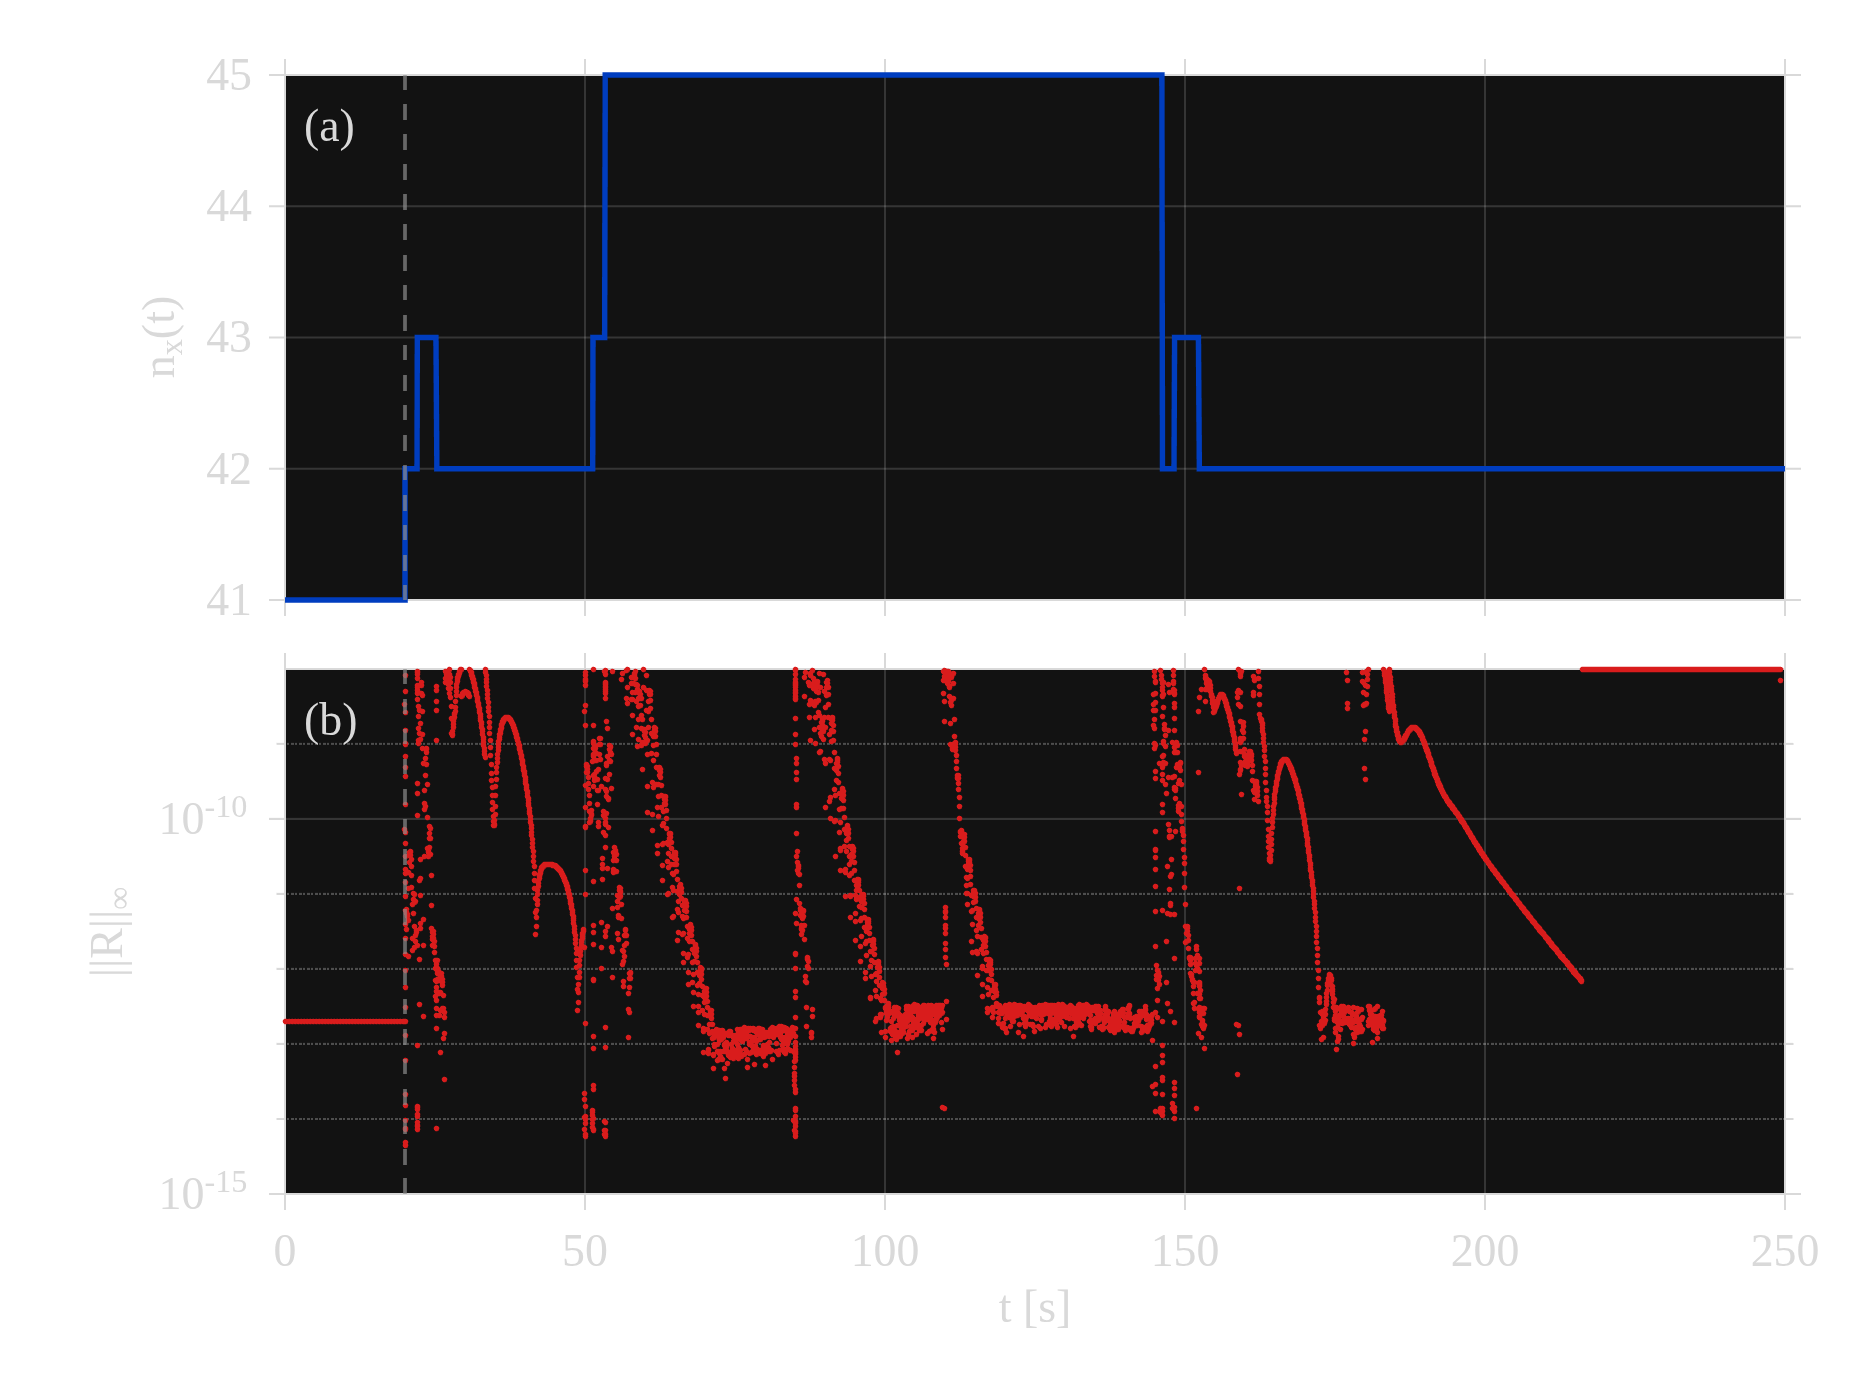
\includegraphics[width=6.20in]{figures/switch_ieee14_new/state_switch_dimension.png}}
 {\fbox{\parbox{6.0in}{\centering\vspace{3em}\ttfamily state\_switch\_dimension.png\\[4pt]
   \normalfont รอการสร้างรูปใหม่
   (รัน \texttt{generate\_switch\_new\_report\_figures}).\vspace{3em}}}}
\caption{(a) จำนวนสเตตเชิงอนุพันธ์ที่ระบบรวมอินทิเกรตจริง $n_x(t)$ วาดเป็นเส้นขั้น
บันได อ่านจากแผนที่สเตตของอุปกรณ์เองที่ทุกจุดตัวอย่างที่ยอมรับ (b) เรซิดวลของแต่ละ
ขั้นเวลาที่ยอมรับ $\lVert R\rVert_\infty$ บนสเกลลอการิทึม เส้นประแนวตั้งสีเทาคือเวลา
ที่ SG ถูกตัดออก ทุกจุดเป็นค่าดิบที่ตัวแก้ยอมรับจากวิถี 250 วินาทีของแขนสลับอัตโนมัติ}
\label{fig:nx}
\end{figure}

%=============================================================================
\section{ผลการไหลของกำลัง}\label{sec:pf}
%=============================================================================
ตารางที่~\ref{tab:pfbus} คือผลการไหลของกำลังที่แก้ได้ในสภาวะ SG ออนไลน์ (เป็นจุด
ทำงานอ้างอิงที่ใช้ดึงค่า $V_i^{\star}$ ในสมการ~\eqref{eq:jvjf}) และ
ตารางที่~\ref{tab:pfline} คือกำลังไหลในกิ่งสายและกำลังสูญเสียที่จุดทำงานเดียวกัน
บัสอ้างอิงจ่าย $P_g=1.3319\pu$ และ $Q_g=-0.1957\pu$ ส่วนบัส IBR ทั้งสี่ (2, 3, 6
และ 8) อัดกำลังตามค่าสั่งของตน ขณะที่บัสโหลดทุกบัสได้รับ $P_L,Q_L$ ครบตามต้องการ

\emph{วิธีอ่านสองตารางนี้} สามสิ่งที่ควรชี้ให้ผู้ฟังเห็น หนึ่ง คอลัมน์ $|V|$ ของ
ตารางที่~\ref{tab:pfbus} คือที่มาของ $V_i^{\star}$ รายบัส สังเกตว่าบัส 6 และบัส 8 มี
แรงดันสูงกว่า $1\pu$ ในสภาวะปกติ จึงยืนยันเหตุผลที่ดัชนี $J_V$ ต้องอ้างค่ารายบัส
สอง คอลัมน์ $Q_{min},Q_{max}$ คือขอบเขตกำลังรีแอกทีฟที่ถูกลงทะเบียนและถูกบังคับใช้
จริงในการแก้ (ไม่ใช่ $\pm\infty$) สาม คอลัมน์ $P_{loss},Q_{loss}$ ในตาราง
ที่~\ref{tab:pfline} คือกำลังสูญเสียในกิ่งสาย ซึ่งค่า $Q_{loss}$ ที่เป็นลบหมายถึงกิ่ง
นั้นจ่ายกำลังรีแอกทีฟสุทธิจากตัวเก็บประจุขนานของสาย ไม่ใช่ความผิดพลาดของเครื่องหมาย

\begin{table}[H]
\centering\footnotesize
\caption{ผลการไหลของกำลังรายบัสที่จุดทำงาน SG ออนไลน์ (ค่าต่อหน่วยบนฐานระบบ
มุมเป็นองศา)}
\label{tab:pfbus}
\IfFileExists{figures/switch_ieee14/table_pf_bus_results.tex}
 {% Generated by scripts/reporting/generate_ieee14_switch_report_figures.m.
\begin{tabular}{rrrrrrrr}\toprule
Bus & Type & $|V|$ & $\theta$ (deg) & $P_g$ & $Q_g$ & $P_L$ & $Q_L$ \\ \midrule
1 & REF & 1.06000 & +0.0000 & +2.32393 & -0.16549 & 0.00000 & 0.00000 \\ 
2 & PV & 1.04500 & -4.9826 & +0.40000 & +0.43557 & 0.21700 & 0.12700 \\ 
3 & PV & 1.01000 & -12.7251 & +0.00000 & +0.25075 & 0.94200 & 0.19000 \\ 
4 & PQ & 1.01767 & -10.3129 & +0.00000 & +0.00000 & 0.47800 & -0.03900 \\ 
5 & PQ & 1.01951 & -8.7739 & +0.00000 & +0.00000 & 0.07600 & 0.01600 \\ 
6 & PV & 1.07000 & -14.2209 & -0.00000 & +0.12731 & 0.11200 & 0.07500 \\ 
7 & PQ & 1.06152 & -13.3596 & +0.00000 & +0.00000 & 0.00000 & 0.00000 \\ 
8 & PV & 1.09000 & -13.3596 & +0.00000 & +0.17623 & 0.00000 & 0.00000 \\ 
9 & PQ & 1.05593 & -14.9385 & +0.00000 & +0.00000 & 0.29500 & 0.16600 \\ 
10 & PQ & 1.05098 & -15.0973 & +0.00000 & +0.00000 & 0.09000 & 0.05800 \\ 
11 & PQ & 1.05691 & -14.7906 & +0.00000 & +0.00000 & 0.03500 & 0.01800 \\ 
12 & PQ & 1.05519 & -15.0756 & +0.00000 & +0.00000 & 0.06100 & 0.01600 \\ 
13 & PQ & 1.05038 & -15.1563 & +0.00000 & +0.00000 & 0.13500 & 0.05800 \\ 
14 & PQ & 1.03553 & -16.0336 & +0.00000 & +0.00000 & 0.14900 & 0.05000 \\ 
\bottomrule\end{tabular}
}
 {\centering\ttfamily table\_pf\_bus\_results.tex รอการสร้างใหม่}
\end{table}

\begin{table}[H]
\centering\footnotesize
\caption{กำลังไหลในกิ่งสายและกำลังสูญเสียที่จุดทำงาน SG ออนไลน์}
\label{tab:pfline}
\IfFileExists{figures/switch_ieee14/table_pf_line_results.tex}
 {% Generated by scripts/reporting/generate_ieee14_switch_report_figures.m.
\begin{tabular}{r@{\hspace{0.8em}}r@{\hspace{0.8em}}r@{\hspace{0.8em}}r@{\hspace{0.8em}}r@{\hspace{0.8em}}r@{\hspace{0.8em}}r}\toprule
Line & From & To & $P_{from}$ & $Q_{from}$ & $P_{loss}$ & $Q_{loss}$ \\ \midrule
1 & 1 & 2 & +0.900928 & -0.203057 & +0.014518 & -0.014696 \\
2 & 1 & 5 & +0.418019 & -0.066451 & +0.008475 & -0.019813 \\
3 & 2 & 3 & +0.464318 & -0.000621 & +0.009133 & -0.009246 \\
4 & 2 & 4 & +0.314334 & -0.079982 & +0.005358 & -0.021354 \\
5 & 2 & 5 & +0.209348 & -0.060569 & +0.002332 & -0.031219 \\
6 & 3 & 4 & -0.197092 & -0.022968 & +0.002456 & -0.007604 \\
7 & 4 & 5 & -0.447907 & +0.102332 & +0.002561 & +0.008079 \\
8 & 4 & 7 & +0.017005 & -0.115901 & +0.000000 & +0.002495 \\
9 & 4 & 9 & +0.062330 & -0.021423 & +0.000000 & +0.002062 \\
10 & 5 & 6 & +0.090091 & +0.002266 & -0.000000 & +0.001610 \\
11 & 6 & 11 & +0.130988 & +0.058687 & +0.001540 & +0.003226 \\
12 & 6 & 12 & +0.085939 & +0.026725 & +0.000784 & +0.001631 \\
13 & 6 & 13 & +0.207419 & +0.084233 & +0.002610 & +0.005140 \\
14 & 7 & 8 & -0.268840 & -0.133746 & +0.000000 & +0.013242 \\
15 & 7 & 9 & +0.285846 & +0.015351 & +0.000000 & +0.007516 \\
16 & 9 & 10 & -0.003741 & +0.022196 & +0.000013 & +0.000036 \\
17 & 9 & 14 & +0.056917 & +0.023544 & +0.000403 & +0.000857 \\
18 & 10 & 11 & -0.093754 & -0.035839 & +0.000693 & +0.001622 \\
19 & 12 & 13 & +0.024155 & +0.009094 & +0.000119 & +0.000108 \\
20 & 13 & 14 & +0.093845 & +0.030080 & +0.001359 & +0.002767 \\
\bottomrule\end{tabular}
}
 {\centering\ttfamily table\_pf\_line\_results.tex รอการสร้างใหม่}
\end{table}

%=============================================================================
\section{สเปกตรัมสัญญาณขนาดเล็ก}\label{sec:sssa}
%=============================================================================
ตารางโมดัลด้านล่างแสดงค่าลักษณะเฉพาะ (eigenvalue) ของสัญญาณขนาดเล็กที่การจัดรูป
หลังการรบกวนแบบตัวแทนหนึ่งกรณี (มี IBR หนึ่งตัวเป็น GFM และสามตัวเป็น GFL) โดยแสดง
ลำดับที่ ค่าลักษณะเฉพาะ $\lambda$ ความถี่โมดัล $f$ และอุปกรณ์กับสเตตที่มีส่วนร่วม
เด่นที่สุดหนึ่งตัว คู่สังยุค (conjugate pair) พิมพ์เพียงแถวเดียว ตารางนี้คือตารางที่
ตัวสร้างผลิตไว้เอง ไม่ใช่สำเนาที่พิมพ์เรียงใหม่ จึงเป็นตารางเดียวกับที่รายงานฉบับ
ภาษาอังกฤษใช้ และตัวเลขตรงกันบิตต่อบิต

\emph{วิธีอ่านตารางโมดัล} นิยามที่ใช้คือ $f_i=|\Im\lambda_i|/2\pi$ และ
$\zeta_i=-\Re\lambda_i/|\lambda_i|$ ดังนั้นค่าลักษณะเฉพาะที่เป็นจำนวนจริงจะมี
$f=0$ และ $\zeta=1$ ตามนิยาม ไม่ใช่เพราะถูกปรับแต่ง สิ่งที่ควรสังเกตเป็นกลุ่มคือ
โมดที่มีความถี่สูงระดับร้อยเฮิรตซ์เป็นกลุ่มของกระแสตัวกรองและเครือข่าย รากจริงสี่ราก
ที่อยู่เหนือ $-100~\mathrm{s}^{-1}$ ขึ้นมาเล็กน้อยคือครอบครัวของบัส DC ทั้งสี่ตัว และ
โมดที่ช้าที่สุดคือกลุ่มตัวอินทิเกรตของวงรอบแรงดัน ซึ่งเป็นตัวกำหนดขอบของอัตราการหน่วง
ในการจัดรูปนี้

\paragraph{โมดของบัส DC เป็นการตรวจสอบแบบจำลอง ไม่ใช่ข้อสังเกตที่ได้มาฟรี}
คอนเวอร์เตอร์แต่ละตัวให้พิกัดบัส DC มาหนึ่งตัว และด้วยแหล่งจ่าย DC ไม่อุดมคติใน
หัวข้อ~\ref{sec:ibr} พิกัดนั้นเป็นสเตตที่มีชีวิตซึ่งผูกกับสเตตด้าน AC ผ่านกำลังของ
คอนเวอร์เตอร์ $P_{ac}$ ค่าลักษณะเฉพาะของมันถูก\emph{ทำนายไว้ก่อน}คำนวณสเปกตรัม โดย
การเชิงเส้นแถว DC ขณะปิดชอปเปอร์ ซึ่งด้วย $C_{dc}=R_{dc}=0.10$ ย่อลงเป็นข้อความที่
พิสูจน์เท็จได้ว่า $\lambda_{dc}=-(1/C)\bigl(1/R_{dc}-P_{ac}/V_{dc}^{2}\bigr)
=-100+10\,P_{ac}/V_{dc}^{2}~\mathrm{s^{-1}}$ ดังนั้นแถว DC ทั้งสี่ต้องเป็นจำนวนจริง
ต้องอยู่เหนือ $-100~\mathrm{s^{-1}}$ ขึ้นมาเล็กน้อย และต้อง\emph{แยกจากกันและเรียง
ตามกำลังที่คอนเวอร์เตอร์แต่ละตัวรับ} --- ยิ่งบัสรับภาระมาก โมดยิ่งลบน้อยลง เพราะพจน์
ที่สองคือความต้านทานส่วนเพิ่มค่าลบของโหลดกำลังคงที่ ตารางเป็นไปตามทั้งสามข้อ: สี่แถว
เป็นค่าที่แยกจากกันโดยมีแรงดันบัส DC เป็นสเตตเด่น และการผกผันความสัมพันธ์ข้างต้นคืนค่า
กำลังรายคอนเวอร์เตอร์ในช่วง $0.3\text{--}0.9$~pu ซึ่งเป็นภาระเดียวกับที่รูปโดเมนเวลา
แสดงสำหรับอุปกรณ์เดียวกัน ไม่มีการปรับค่าใดเพื่อให้ได้ความสอดคล้องนี้ closure ถูก
อนุมานก่อน แล้วจึงคำนวณสเปกตรัมทีหลัง

\paragraph{สิ่งที่ถูกแทนที่}
รายงานฉบับก่อนหน้านี้พิมพ์สี่แถวที่ $\lambda=-10.000000$ พอดี โดยมีความถี่โมดัลเป็น
ศูนย์ อัตราการหน่วงเท่าหนึ่ง และค่าการมีส่วนร่วมเท่ากับ $1.000$ พอดีบนแรงดันบัส DC
นั่นไม่ใช่ความบังเอิญและไม่ใช่สิ่งแปลกปลอมเชิงตัวเลข แต่เป็นลายเซ็นของ closure
อุดมคติฉบับก่อน: มันทำให้แถว DC ถูกแยกออกจากกันโดยสมบูรณ์ ดังนั้น $-1/T_{dc}$ จึงเป็น
ค่าลักษณะเฉพาะที่มีพหุคูณเชิงพีชคณิตเท่าสี่ เวกเตอร์หนึ่งหน่วยบนพิกัดนั้นเป็นเวกเตอร์
ลักษณะเฉพาะซ้ายพอดี และค่าการมีส่วนร่วมจึงเท่ากับหนึ่งพอดีในเชิงพีชคณิต ความอุดมคติ
เดียวกันนี้ยังตรึง $V_{dc}$ ให้คงที่ตลอดวิถี ทั้งสองอย่างถูกกำจัดไปแล้วโดย closure
ปัจจุบัน และสี่แถวนั้นไม่ควรปรากฏอีก

\begin{center}\footnotesize
\IfFileExists{figures/switch_ieee14/sssa_modes_n1.tex}
 {% Physical decision spectrum; conjugate pairs printed once.
% nGFM=1 selected=5 reference=5 full=45 physical=44 method=common_gfm_vsg_angle_quotient
\begingroup\small\setlength{\tabcolsep}{3pt}
\begin{longtable}{@{}r p{0.25\textwidth} r r p{0.35\textwidth}@{}}
\toprule
No. & Eigenvalue $\lambda$ (s$^{-1}$) & $f$ (Hz) & $\zeta$ & Dominant participation: device:state (normalised) \\ \midrule
\endfirsthead
\toprule
No. & Eigenvalue $\lambda$ (s$^{-1}$) & $f$ (Hz) & $\zeta$ & Dominant participation: device:state (normalised) \\ \midrule
\endhead
1 & $-3881.470073+\mathrm{j}1061.916124$ & $169.009200$ & $0.964553$ & IBR6:$i_d$ (0.131); IBR6:$i_q$ (0.131); IBR8:$i_d$ (0.129) \\
2 & $-159.046981$ & $0$ & $1.000000$ & IBR8:$E^{GFM}$ (0.992); IBR8:$V_{d,del}^{GFM}$ (0.006); IBR8:$\xi_{Id}^{GFM}$ (0.001) \\
3 & $-156.112829+\mathrm{j}816.094065$ & $129.885404$ & $0.187886$ & IBR6:$i_d$ (0.305); IBR6:$i_q$ (0.305); IBR3:$i_d$ (0.105) \\
4 & $-140.724047+\mathrm{j}1033.942353$ & $164.557036$ & $0.134861$ & IBR8:$i_q$ (0.344); IBR8:$i_d$ (0.343); IBR3:$i_d$ (0.062) \\
5 & $-106.207976+\mathrm{j}615.792052$ & $98.006349$ & $0.169964$ & IBR2:$i_d$ (0.248); IBR2:$i_q$ (0.248); IBR3:$i_d$ (0.168) \\
6 & $-17.922231$ & $0$ & $1.000000$ & IBR8:$\omega_{VSG}^{GFM}$ (0.909); IBR8:$\xi_{Id}^{GFM}$ (0.017); IBR6:$\xi_{Id}^{GFL}$ (0.011) \\
7 & $-13.345138+\mathrm{j}1.527324$ & $0.243081$ & $0.993514$ & IBR2:$\xi_{Id}^{GFL}$ (0.261); IBR2:$\xi_{Iq}^{GFL}$ (0.261); IBR3:$\xi_{Iq}^{GFL}$ (0.171) \\
8 & $-13.151005+\mathrm{j}2.154763$ & $0.342941$ & $0.986841$ & IBR6:$\xi_{Id}^{GFL}$ (0.281); IBR6:$\xi_{Iq}^{GFL}$ (0.280); IBR3:$\xi_{Iq}^{GFL}$ (0.106) \\
9 & $-12.633262+\mathrm{j}3.598177$ & $0.572668$ & $0.961751$ & IBR8:$\xi_{Id}^{GFM}$ (0.227); IBR8:$\xi_{Iq}^{GFM}$ (0.223); IBR8:$V_{d,del}^{GFM}$ (0.062) \\
10 & $-11.446947+\mathrm{j}14.627753$ & $2.328079$ & $0.616280$ & IBR8:$V_{d,del}^{GFM}$ (0.155); IBR8:$\xi_{Id}^{GFM}$ (0.142); IBR6:$V_{d,del}^{GFL}$ (0.099) \\
11 & $-10.000000$ & $0$ & $1.000000$ & IBR2:$V_{dc}$ (1.000); IBR2:$i_d$ (0.000); IBR2:$i_q$ (0.000) \\
12 & $-10.000000$ & $0$ & $1.000000$ & IBR3:$V_{dc}$ (1.000); IBR2:$i_d$ (0.000); IBR2:$i_q$ (0.000) \\
13 & $-10.000000$ & $0$ & $1.000000$ & IBR6:$V_{dc}$ (1.000); IBR2:$i_d$ (0.000); IBR2:$i_q$ (0.000) \\
14 & $-10.000000$ & $0$ & $1.000000$ & IBR8:$V_{dc}$ (1.000); IBR2:$i_d$ (0.000); IBR2:$i_q$ (0.000) \\
15 & $-6.988836+\mathrm{j}12.831357$ & $2.042174$ & $0.478320$ & IBR8:$V_{q,del}^{GFM}$ (0.155); IBR8:$\xi_{Iq}^{GFM}$ (0.145); IBR6:$V_{q,del}^{GFL}$ (0.094) \\
16 & $-6.293824+\mathrm{j}109.583760$ & $17.440797$ & $0.057339$ & IBR2:$V_{d,del}^{GFL}$ (0.224); IBR2:$V_{q,del}^{GFL}$ (0.223); IBR3:$V_{q,del}^{GFL}$ (0.146) \\
17 & $-2.508684+\mathrm{j}84.237836$ & $13.406868$ & $0.029768$ & IBR6:$V_{d,del}^{GFL}$ (0.256); IBR6:$V_{q,del}^{GFL}$ (0.253); IBR3:$V_{q,del}^{GFL}$ (0.101) \\
18 & $-2.048337$ & $0$ & $1.000000$ & IBR6:$\xi_{P}^{GFL}$ (0.289); IBR2:$\xi_{P}^{GFL}$ (0.235); IBR3:$\xi_{P}^{GFL}$ (0.212) \\
19 & $-1.643720+\mathrm{j}47.532682$ & $7.565061$ & $0.034560$ & IBR8:$V_{d,del}^{GFM}$ (0.219); IBR8:$V_{q,del}^{GFM}$ (0.214); IBR8:$\xi_{Id}^{GFM}$ (0.060) \\
20 & $-1.509781$ & $0$ & $1.000000$ & IBR6:$\xi_{Q}^{GFL}$ (0.321); IBR6:$\xi_{P}^{GFL}$ (0.265); IBR3:$\xi_{P}^{GFL}$ (0.128) \\
21 & $-1.503650+\mathrm{j}0.674893$ & $0.107413$ & $0.912318$ & IBR8:$\xi_{Vq}^{GFM}$ (0.286); IBR6:$\xi_{Q}^{GFL}$ (0.122); IBR8:$\xi_{Vd}^{GFM}$ (0.111) \\
22 & $-1.443329$ & $0$ & $1.000000$ & IBR3:$\xi_{P}^{GFL}$ (0.299); IBR2:$\xi_{P}^{GFL}$ (0.275); IBR2:$\xi_{Q}^{GFL}$ (0.227) \\
23 & $-1.407957$ & $0$ & $1.000000$ & IBR2:$\xi_{Q}^{GFL}$ (0.343); IBR2:$\xi_{P}^{GFL}$ (0.288); IBR6:$\xi_{P}^{GFL}$ (0.157) \\
24 & $-1.390336$ & $0$ & $1.000000$ & IBR3:$\xi_{Q}^{GFL}$ (0.376); IBR3:$\xi_{P}^{GFL}$ (0.246); IBR6:$\xi_{P}^{GFL}$ (0.176) \\
25 & $-0.746742$ & $0$ & $1.000000$ & IBR8:$\xi_{Vd}^{GFM}$ (0.624); IBR6:$\xi_{P}^{GFL}$ (0.087); IBR2:$\xi_{P}^{GFL}$ (0.082) \\
26 & $-0.619437+\mathrm{j}2.216829$ & $0.352819$ & $0.269116$ & IBR6:$\delta_{PLL}^{GFL}$ (0.278); IBR6:$\xi_{PLL}^{GFL}$ (0.277); IBR2:$\delta_{PLL}^{GFL}$ (0.196) \\
27 & $-0.605533+\mathrm{j}2.186111$ & $0.347930$ & $0.266940$ & IBR3:$\delta_{PLL}^{GFL}$ (0.305); IBR3:$\xi_{PLL}^{GFL}$ (0.304); IBR2:$\delta_{PLL}^{GFL}$ (0.149) \\
28 & $-0.175750+\mathrm{j}2.159250$ & $0.343655$ & $0.081126$ & IBR3:$\delta_{PLL}^{GFL}$ (0.136); IBR2:$\delta_{PLL}^{GFL}$ (0.133); IBR6:$\delta_{PLL}^{GFL}$ (0.128) \\
\bottomrule
\end{longtable}\endgroup
}
 {\ttfamily sssa\_modes\_n1.tex รอการสร้างใหม่
  (รัน \texttt{generate\_gfl\_gfm\_sssa\_tables}).}
\end{center}

สเปกตรัมทั้งหมดอยู่ในระนาบครึ่งซ้ายที่การจัดรูปนี้ ข้อความนี้เป็นข้อความเกี่ยวกับ
สัญญาณขนาดเล็ก ณ \emph{จุดเชิงเส้นหนึ่งจุด}เท่านั้น ไม่ใช่ และต้องไม่ถูกอ่านว่าเป็น
ใบรับรองเสถียรภาพของวิถีแบบสลับโหมดทั้งเส้น เหตุผลคือการวิเคราะห์สัญญาณขนาดเล็ก
สมมติว่าการรบกวนเล็กพอที่การประมาณเชิงเส้นยังใช้ได้ ขณะที่ฟอลต์และการสลับโหมดใน
งานนี้เป็นการรบกวนขนาดใหญ่โดยธรรมชาติ ทั้งสองเครื่องมือจึงเสริมกัน ไม่ทดแทนกัน

%=============================================================================
\section{ผลตอบสนองชั่วครู่: การจำลองในโดเมนเวลา}\label{sec:transient}
%=============================================================================
รูปที่~\ref{fig:periods} วางไทม์ไลน์หกช่วงไว้เหนือกราฟผลลัพธ์ทั้งหมดของหัวข้อนี้
เพื่อให้เทียบเวลาเหตุการณ์กับเส้นกราฟได้โดยตรง

\begin{figure}[H]
\centering
\begin{tikzpicture}[
  font=\normalsize,
  per/.style={circle,draw,thick,minimum size=2.5cm,inner sep=2pt,
    align=center,text=white,font=\bfseries},
  tlbl/.style={font=\small},
  tlab/.style={midway,above,font=\small},
  tlabb/.style={midway,below,font=\small},
  arr/.style={-{Latex[length=3mm]},very thick,color=blue!60!black}]

\node[per,fill=pgreen] (p1) at (0,0)     {ช่วง 1\\ ทำงาน\\ ปกติ};
\node[per,fill=pred]   (p2) at (4.4,0)   {ช่วง 2\\ ตัด $SG_1$\\ (เสีย slack)};
\node[per,fill=pblue]  (p3) at (8.8,0)   {ช่วง 3\\ โหลด $P,Q$\\ เพิ่ม $+20\%$};
\node[per,fill=pred]   (p4) at (8.8,-4.4){ช่วง 4\\ ฟอลต์\\ ที่บัส 9};
\node[per,fill=pyellow](p5) at (4.4,-4.4){ช่วง 5\\ เปิดสาย\\ 6--13};
\node[per,fill=pblue]  (p6) at (0,-4.4)  {ช่วง 6\\ ต่อกลับ\\ $SG_1$};

\draw[arr] (-3.2,0) -- node[tlab]{$t=0\second$} (p1);
\draw[arr] (p1) -- node[tlab]{$t=20\second$} (p2);
\draw[arr] (p2) -- node[tlab]{$t=50\second$} (p3);
\draw[arr] (p3) -- node[font=\small,left=2mm,pos=0.5,align=right]{$t=85.000$\\--$85.150\second$} (p4);
\draw[arr] (p4) -- node[tlabb]{$t=110\second$} (p5);
\draw[arr] (p5) -- node[tlabb]{$t=145\second$} (p6);
\draw[arr] (p6) -- node[tlabb,pos=0.62]{$t\to\NewRunEnd\second$} ++(-3.2,0);

\node[tlbl,below=3pt of p6,align=center,text=black]
  {ต่อกลับที่ $\NewRunReclose\second$\\ ปลดโหมดครั้งแรกที่ $\NewRunFirstRelease\second$};
\end{tikzpicture}
\caption{ลำดับเหตุการณ์รบกวนหกช่วง สีเขียว: ยังไม่ถูกรบกวน สีแดง: เหตุการณ์ที่
ทำให้สูญเสียแหล่งจ่ายหรือทำให้บัสเกิดฟอลต์ สีเหลือง: การเปลี่ยนโครงสร้างเครือข่าย
สีน้ำเงิน: การกระทำเพื่อฟื้นฟูระบบ เวลาที่ตั้งไว้ล่วงหน้า ($0$, $20$, $50$,
$85.000$--$85.150$, $110$, $145\second$) เป็นค่าจากกรณีศึกษา ส่วนเวลาต่อกลับและ
เวลาปลดโหมดครั้งแรกอ่านจากบันทึกเหตุการณ์ที่ตัวแก้ยอมรับ}
\label{fig:periods}
\end{figure}

ตารางที่~\ref{tab:runscalars} รวมตัวเลขสรุปของการรันที่ใช้วาดกราฟทุกรูป
ในหัวข้อนี้ ตัวเลขทั้งหมดเป็นค่าที่ตัวแก้ยอมรับจากวิถี $\NewRunEnd$ วินาทีของแขน
สลับโหมดอัตโนมัติ และถูกอ่านผ่านมาโครที่ตัวสร้างเขียนให้ ไม่มีตัวเลขใดพิมพ์ตรงลงใน
เนื้อความ ค่าสุดขีดของแรงดันและความถี่ในตารางนี้เป็น\emph{ผลที่รายงาน}
ไม่ใช่เกณฑ์ยอมรับ และไม่ถูกนำไปปรับแบบจำลองย้อนกลับ

\begin{table}[H]
\centering\footnotesize
\caption{ตัวเลขสรุปของการรัน $\NewRunEnd$ วินาทีที่ใช้วาดกราฟในหัวข้อนี้}
\label{tab:runscalars}
\begin{tabularx}{\textwidth}{@{}>{\raggedright\arraybackslash}p{0.40\textwidth}l X@{}}
\toprule
รายการ & ค่า & หมายเหตุ \\ \midrule
เวลาสุดท้ายที่ยอมรับได้ & $\NewRunEnd\second$ & ขอบฟ้าเต็มของการรัน ไม่มีการตัดท้าย \\
สถานะการต่อกลับ & \NewRunRecloseStatus & อ่านจากบันทึกเหตุการณ์ \\
ช่วงแรงดันทุกบัสที่พบ & $\NewRunVMin$--$\NewRunVMax\pu$ & ค่าสุดขีดชั่วครู่ ไม่ใช่พิกัดใช้งาน \\
ช่วงความถี่ที่พบ & $\NewRunFMin$--$\NewRunFMax$~Hz & ค่าสุดขีดชั่วครู่ระหว่างฟอลต์และการสลับโหมด \\
ความถี่จุดศูนย์กลางความเฉื่อยปลายทาง & $\NewRunTerminalF$~Hz & ที่ $t=\NewRunEnd\second$ \\
ช่วงแรงดันปลายทาง & $\NewRunTerminalVMin$--$\NewRunTerminalVMax\pu$ & ที่ $t=\NewRunEnd\second$ \\
เรซิดวลสูงสุดของขั้นที่ยอมรับ & \NewRunResidual & ต่ำกว่าเกณฑ์ $10^{-8}$ ทุกขั้น \\
ระดับการแบ่งขั้นเวลาย่อยที่ลึกสุด & $\NewRunSubdivision$ ชั้น & กลไกแบ่งครึ่งแบบทวิภาค \\
ขั้นทดลองที่ถูกปฏิเสธเพราะออกนอกโดเมน & $\NewRunDomainRejects$ ครั้ง & ไม่มีการผ่อนเกณฑ์เพื่อให้ผ่าน \\
ขั้นเวลาที่ตัวควบคุมปฏิเสธ & $\NewRunRejectedSteps$ ครั้ง & ตัวเดินขั้นแบบ \NewRunStepper \\
จำนวนจุดตัวอย่างที่ยอมรับ & $\NewRunSamples$ & \\
เวลาที่ SG ต่อกลับสำเร็จ & $\NewRunReclose\second$ & อ่านจากบันทึกเหตุการณ์ \\
ส่วนต่างขณะปิดเบรกเกอร์ & $\Delta V=\NewRunSyncDV\pu$ & ผ่านกรอบการซิงโครไนซ์เดิม \\
 & $\Delta f=$ \NewRunSyncDF\ pu & \\
 & $\Delta\theta=\NewRunSyncDTheta^{\circ}$ & \\
เวลาที่เลื่อนโหมดขึ้น ($\NewRunNAugment$ ครั้ง) &
$\NewRunAugmentOne$, $\NewRunAugmentTwo$, & แต่ละครั้งผ่านใบรับรองการเปลี่ยนสภาพ \\
 & $\NewRunAugmentThree$, $\NewRunAugmentFour\second$ & \\
เวลาที่ปลดโหมด ($\NewRunNRelease$ ครั้ง) &
$\NewRunReleaseOne$, $\NewRunReleaseTwo$, & ปลดได้ครั้งละหนึ่งตัว \\
 & $\NewRunReleaseThree\second$ & \\
จำนวน GFM สูงสุดที่ถือพร้อมกัน & $\NewRunGfmMax$ ตัว & ไปถึงแบบเป็นขั้น ไม่ใช่กระโดด \\
สถานะการเลือกชุดใหม่หลังต่อกลับ & \NewRunReselection & fail-closed ที่ถูกต้อง \\
\bottomrule
\end{tabularx}
\end{table}

รูปที่~\ref{fig:pq} แสดงกำลังจริงและกำลังรีแอกทีฟรายตัวของ IBR ตลอดขอบฟ้าเต็ม
$0\text{--}\NewRunEnd\second$ ด้านบนของแผงกำลังมีแถบสถานะเชิงกำกับสองแถบ: แถบบนสุด
คือโหมด GFM/GFL ของ IBR แต่ละตัว และแถบที่สองคือ\emph{เจ้าของแหล่งอ้างอิง}
คืออุปกรณ์ตัวเดียวที่ถือมุมอ้างอิงของเกาะไฟฟ้าไว้ในแต่ละขณะ

โหมดและความเป็นเจ้าของแหล่งอ้างอิงเป็นสัญญาที่\emph{แยกกัน}: IBR หลายตัวเป็น GFM ได้
พร้อมกัน แต่มีเพียงตัวเดียวที่เป็นเจ้าของมุมอ้างอิง ในผลนี้ SG เป็นเจ้าของจนถึง
$t=20\second$ และกลับมาเป็นเจ้าของอีกครั้งหลังการต่อกลับ ช่วงระหว่างนั้น
IBR$_1$ (บัส~2) เป็นผู้นำอ้างอิง เส้นทั้งสี่คือ IBR ทั้งสี่ตัวที่บัส 2, 3, 6 และ 8
ทุกจุดตัวอย่างเป็นค่าดิบที่ตัวแก้ยอมรับ และช่วง $0\text{--}\NewRunEnd\second$
คือขอบฟ้าเต็มของวิถี (ไม่มีการตัดช่วงแสดงผล)

จุดสำคัญของผลชุดนี้อยู่ที่แถบโหมด: ตัวกำกับ\emph{ไม่ได้}ยกทั้งสี่ตัวขึ้นพร้อมกัน
มันเลื่อนขึ้นเป็นขั้น $\NewRunNAugment$ ครั้ง (ที่ $\NewRunAugmentOne$,
$\NewRunAugmentTwo$, $\NewRunAugmentThree$ และ $\NewRunAugmentFour\second$)
จนถือ GFM สูงสุด $\NewRunGfmMax$ ตัว แล้วปลดลง $\NewRunNRelease$ ครั้งหลังการ
ต่อกลับ หัวข้อ~\ref{sec:compare} จะแสดงว่าการ\emph{ตรึง} $\NewRunGfmMax$ ตัวไว้
ตั้งแต่ต้นทำให้ระบบพังก่อนถึงขอบฟ้า ทั้งที่ชุดเดียวกันนั้นผ่านการรับรองเชิงเส้น
นั่นคือเหตุผลที่ลำดับการเลื่อนขึ้นสำคัญไม่แพ้ปลายทาง

\emph{วิธีอ่านรูปที่~\ref{fig:pq}} อ่านจากบนลงล่างเป็นลำดับเหตุ--ผล: แถบโหมดบอกว่า
ตัวกำกับ\emph{ตัดสินใจ}อะไร แถบเจ้าของอ้างอิงบอกว่าใคร\emph{ถือ}มุมอ้างอิงอยู่ และ
แผง (a), (b) บอกว่าผลลัพธ์ทางไฟฟ้า\emph{เป็นอย่างไร}หลังการตัดสินใจนั้น จุดที่ควร
เน้นตอนนำเสนอคือ ที่ $t=20\second$ ทั้งสามแถวเปลี่ยนพร้อมกัน ซึ่งยืนยันว่าเกตกันการ
สูญเสียแหล่งอ้างอิงทำงานก่อนตรรกะเวลาหน่วง ตามที่อธิบายไว้ในหัวข้อ~\ref{sec:sev}

\begin{figure}[H]
\centering
\IfFileExists{figures/switch_ieee14_decision/mode_switch_PQ.png}
 {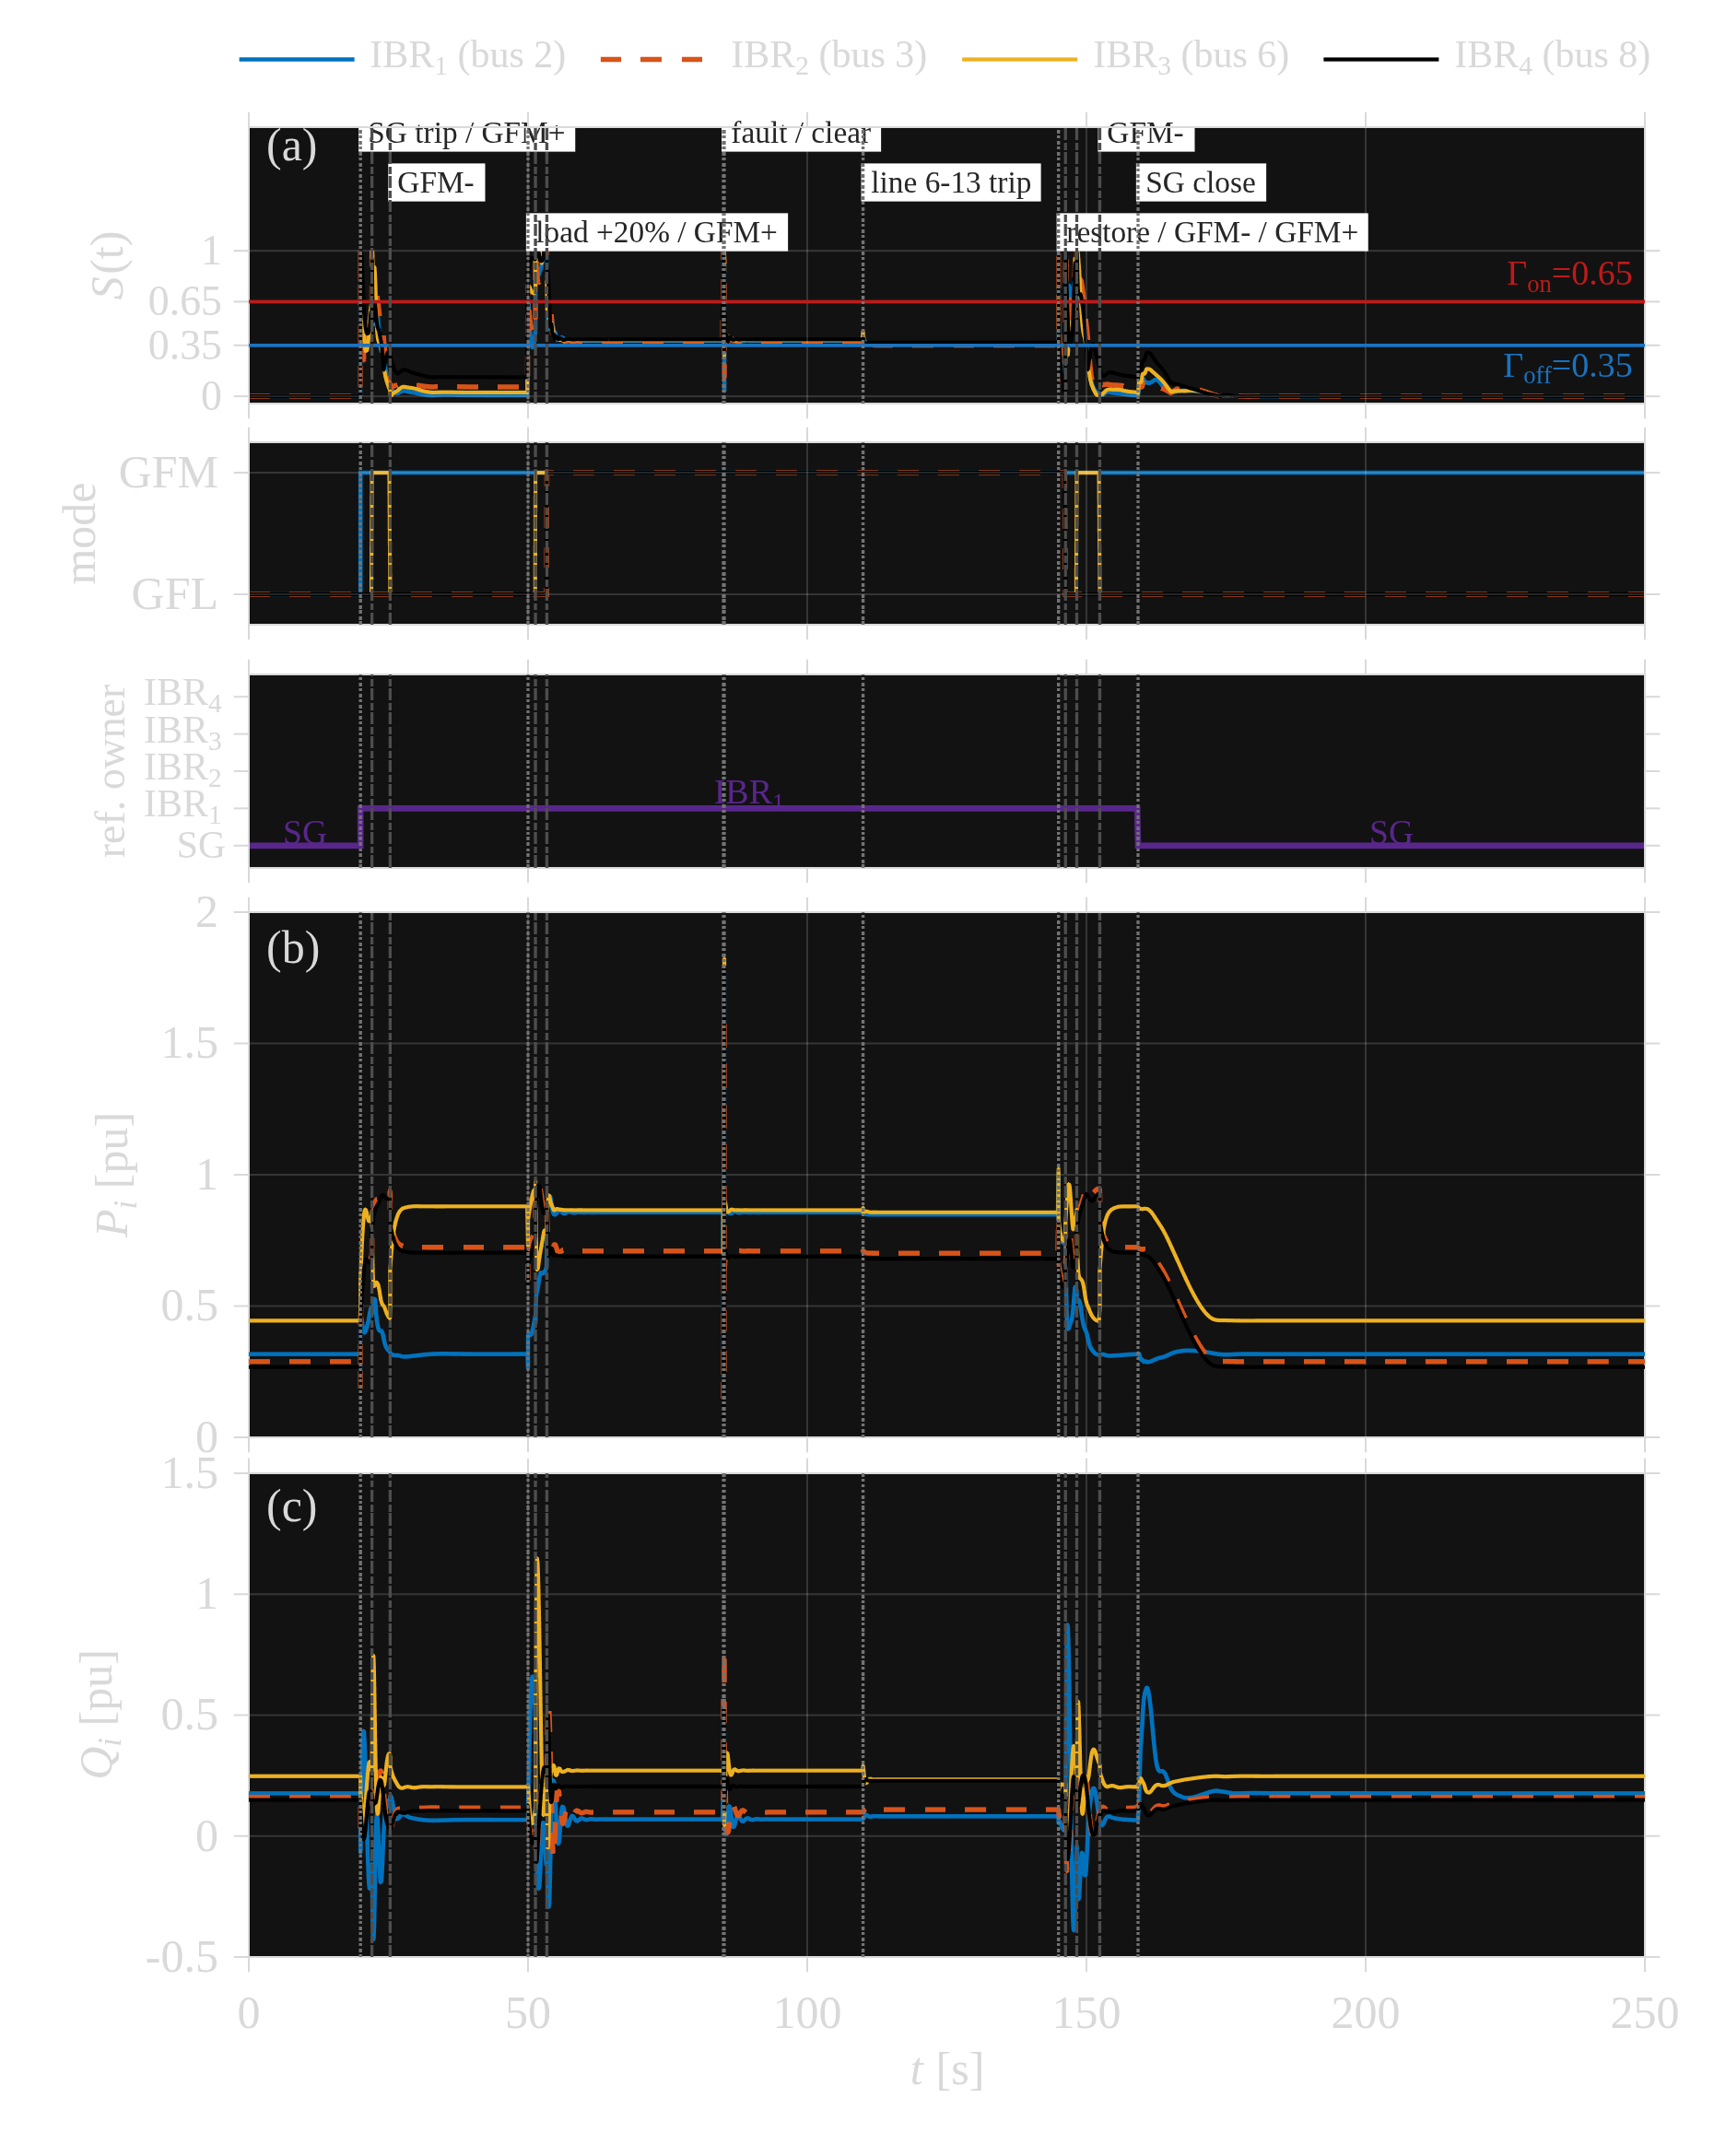
\includegraphics[width=6.20in]{figures/switch_ieee14_decision/mode_switch_PQ.png}}
 {\fbox{\parbox{6.0in}{\centering\vspace{3em}\ttfamily mode\_switch\_PQ.png\\[4pt]
   \normalfont รอการสร้างรูปใหม่
   (รัน \texttt{generate\_ieee14\_mode\_pq\_figure}).\vspace{3em}}}}
\caption{แถบบนสุด: โหมด GFM/GFL ของ IBR แต่ละตัว (ขั้น GFL/GFM สี่เส้นวางทับกัน
ไม่มีการเลื่อนระดับเพื่อการแสดงผล) แถบที่สอง: เจ้าของแหล่งอ้างอิง (อุปกรณ์ที่ถือมุม
อ้างอิงของเกาะไฟฟ้า --- SG แล้วเป็น IBR$_1$ แล้วกลับเป็น SG) (a) กำลังจริงรายตัว
$P_i\pu$ (b) กำลังรีแอกทีฟรายตัว $Q_i\pu$ เส้นประแนวตั้งคือเวลาเหตุการณ์ที่อ่านจาก
ตารางเหตุการณ์และบันทึกที่ยอมรับ ทุกจุดเป็นค่าดิบที่ตัวแก้ยอมรับจากวิถี
$\NewRunEnd$ วินาที ช่วง $t\in[0,\NewRunEnd]\second$ เป็นขอบฟ้าเต็ม}
\label{fig:pq}
\end{figure}

รูปที่~\ref{fig:elec} ขยายภาพให้เห็นตัวแปรทางไฟฟ้าครบแปดแผง เพื่อให้ตรวจสอบได้ว่า
พฤติกรรมที่เห็นในรูปที่~\ref{fig:pq} สอดคล้องกับกระแส แรงดัน มุม และความถี่หรือไม่
แผง (c), (d) คือกระแสในกรอบ $dq$ ซึ่งเป็นที่ที่จะเห็นผลของตัวจำกัดกระแสแบบวงกลม
ชัดที่สุดในช่วงฟอลต์ แผง (e), (f) คือความถี่และมุมเทียบจุดต่อร่วม ซึ่งเป็นตัวชี้ว่า
อุปกรณ์ยังซิงโครไนซ์กันอยู่หรือไม่ และแผง (g), (h) คือแรงดันที่จุดต่อร่วมและแรงดัน
ต่ำสุดของเครือข่าย ซึ่งเป็นตัวแปรที่ป้อนดัชนี $J_V$ โดยตรง

\begin{figure}[H]
\centering
\IfFileExists{figures/switch_ieee14_decision/electrical_adaptive.png}
 {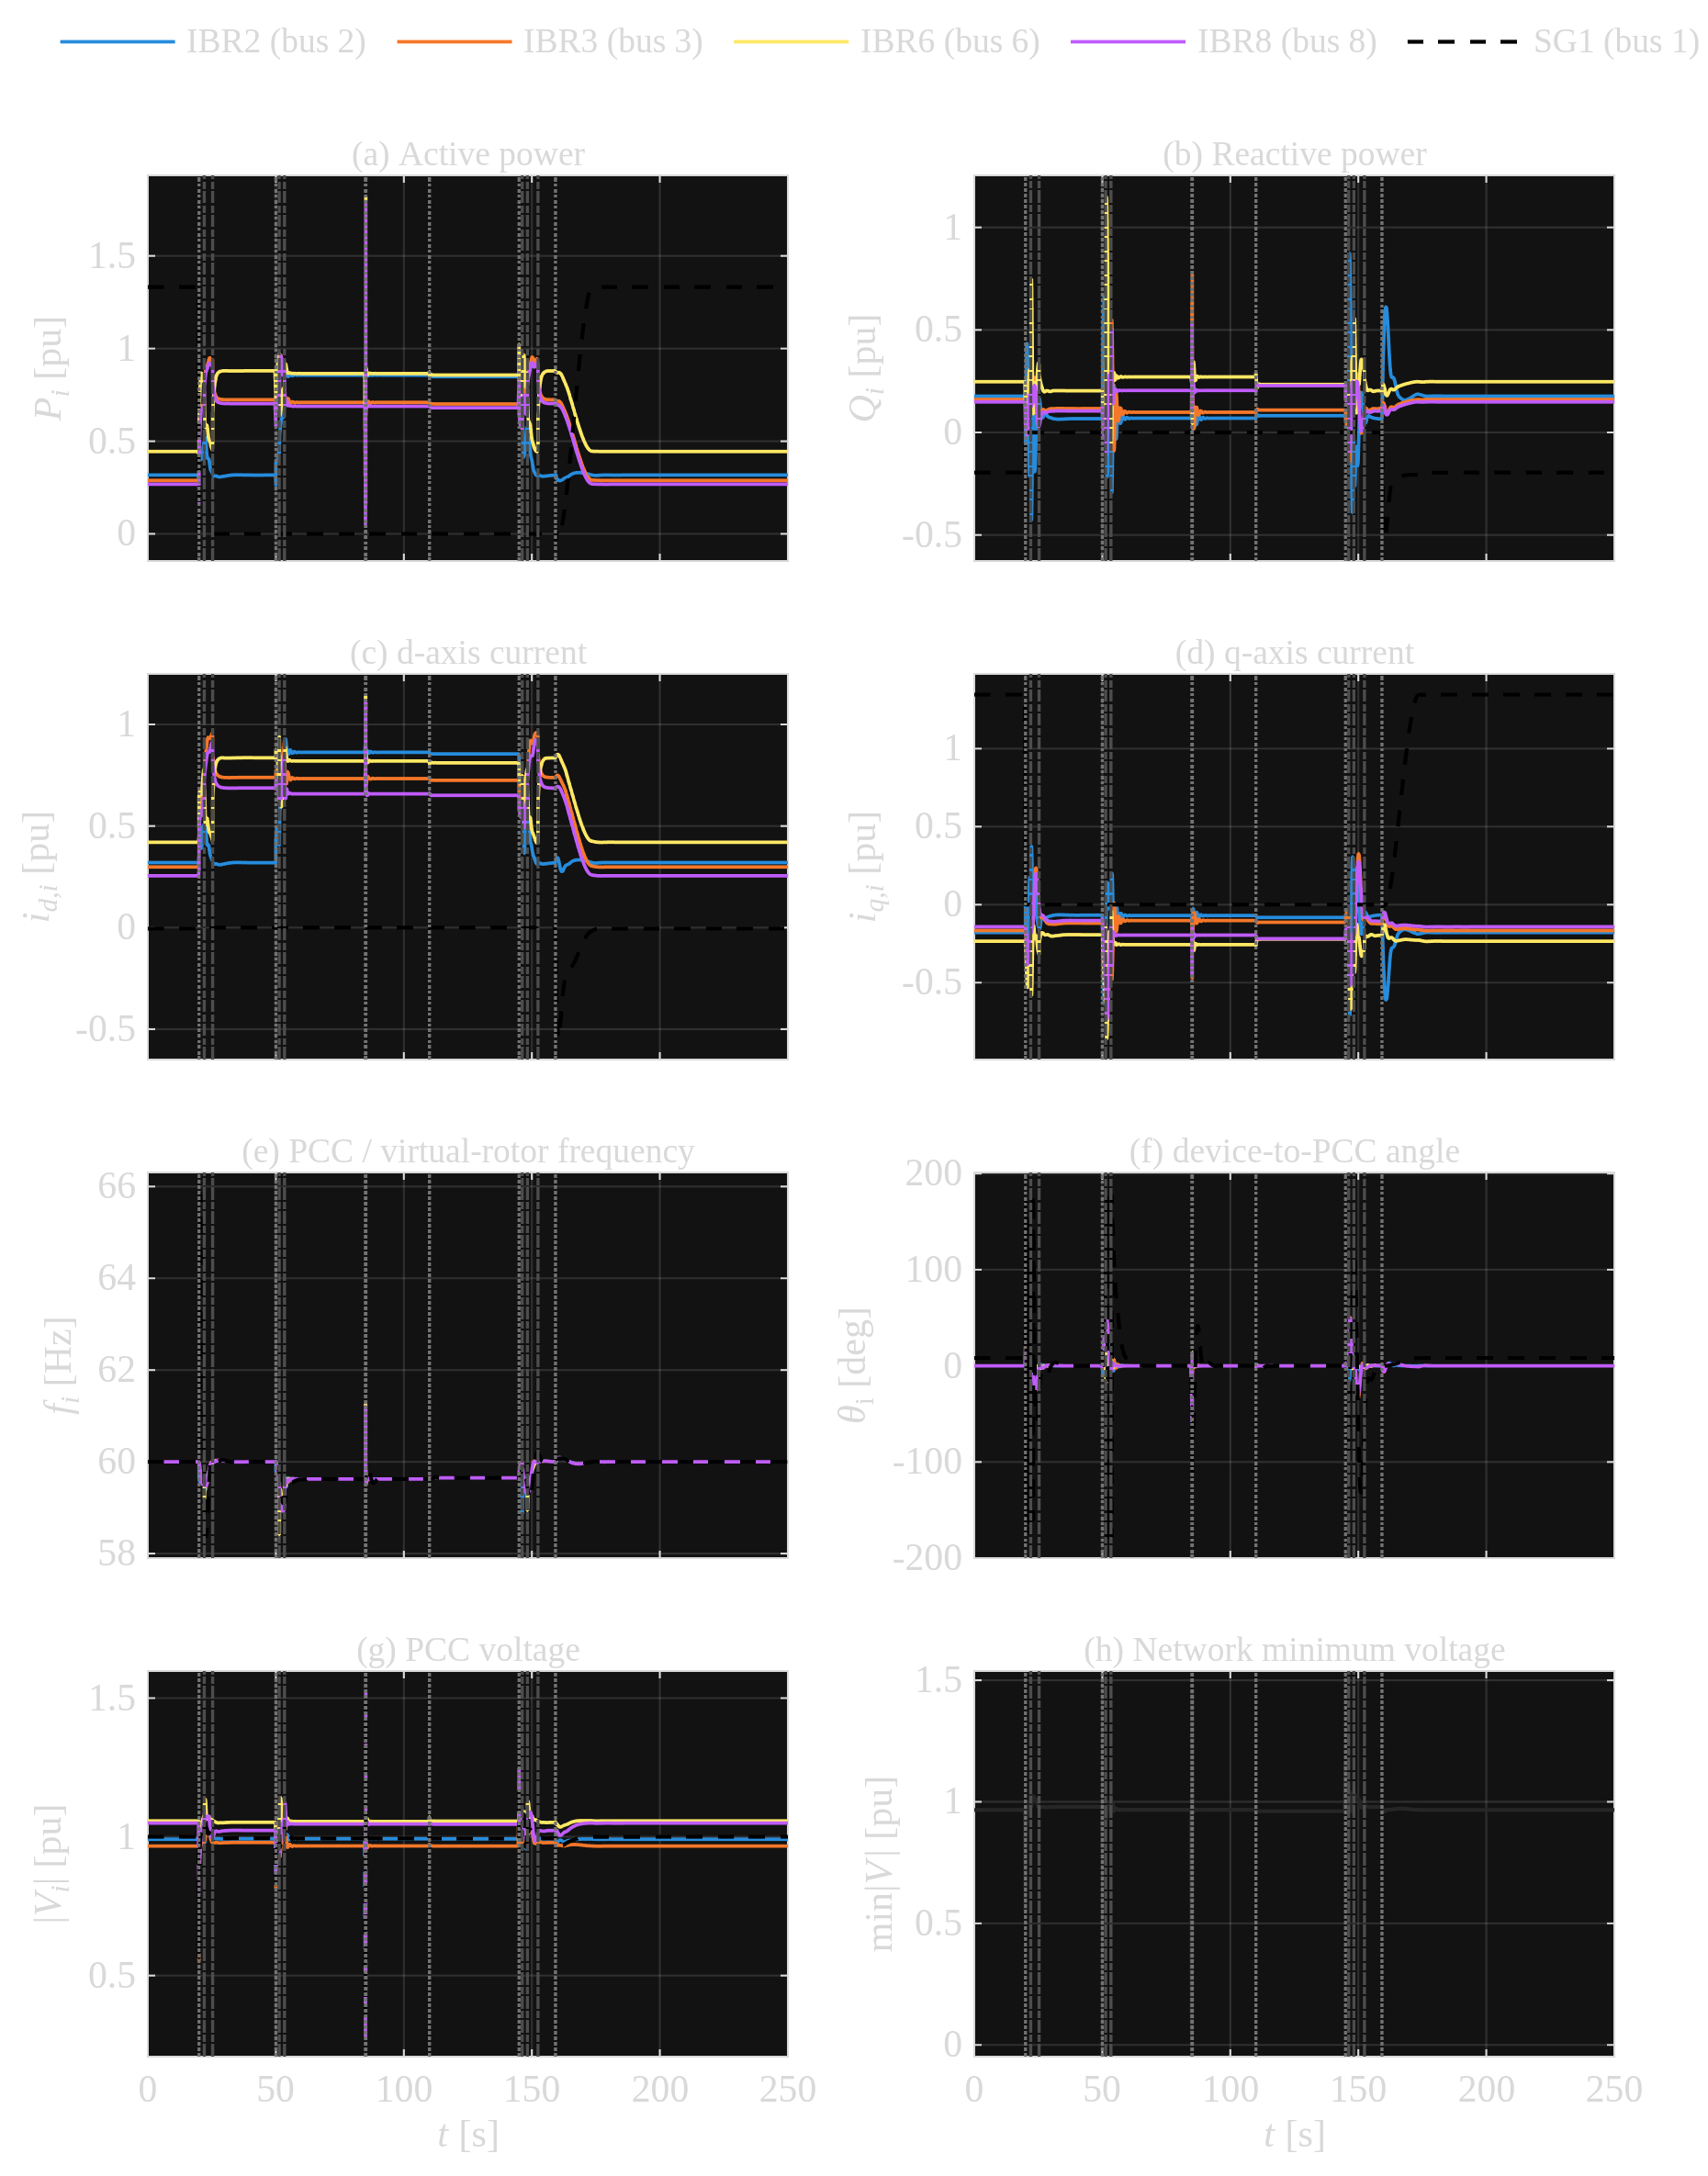
\includegraphics[width=6.20in]{figures/switch_ieee14_decision/electrical_adaptive.png}}
 {\fbox{\parbox{6.0in}{\centering\vspace{3em}\ttfamily electrical\_adaptive.png\\[4pt]
   \normalfont รอการสร้างรูปใหม่
   (รัน \texttt{generate\_ieee14\_switch\_evidence}).\vspace{3em}}}}
\caption{ผลตอบสนองทางไฟฟ้าแปดแผง (ค่าดิบที่ตัวแก้ยอมรับ จากวิถี $\NewRunEnd$ วินาที
ช่วง $t\in[0,\NewRunEnd]\second$ เป็นขอบฟ้าเต็ม) (a) กำลังจริง $P_i$
(b) กำลังรีแอกทีฟ $Q_i$ (c) กระแสแกน $d$ (d) กระแสแกน $q$ (e) ความถี่ที่จุดต่อร่วม
หรือความถี่โรเตอร์เสมือน (f) มุมของอุปกรณ์เทียบจุดต่อร่วม (g) แรงดันที่จุดต่อร่วม
(h) แรงดันต่ำสุดของเครือข่าย IBR ทั้งสี่ใช้สีตามคำอธิบายด้านบนรูป และ SG เป็นเส้น
ดำประในทุกแผงที่มีคู่เทียบ แผง (h) เป็นสเกลาร์ของทั้งระบบจึงมีเส้นเดียวโดยนิยาม}
\label{fig:elec}
\end{figure}

%=============================================================================
\section{การเปรียบเทียบนโยบายควบคุม: ไม่สลับ เทียบ สลับ เทียบ ตรึงไว้คงที่}\label{sec:compare}
%=============================================================================
หัวข้อนี้ตอบคำถามที่ผลชุดเดียวตอบไม่ได้: การให้ IBR สลับโหมดเองมีประโยชน์วัดเป็น
ตัวเลขได้เท่าไร และถ้าเลือกชุด GFM ที่ ``ดีที่สุด'' แล้วตรึงไว้เลยจะดีกว่าหรือไม่
วิธีตอบคือรันวิถีเดิมซ้ำห้าครั้ง โดยใช้เครือข่าย การจ่ายโหลด ตารางเหตุการณ์ ตัวแก้
และตัวควบคุมขั้นเวลา\emph{ชุดเดียวกันทุกตัว} ต่างกันเฉพาะนโยบายควบคุมของ IBR

\subsection{ทำไมการเทียบนี้ถึงเชื่อถือได้}
ตัวรันประกาศรายชื่อฟิลด์ที่แต่ละแขนได้รับอนุญาตให้ต่าง แล้ว\emph{ตรวจสอบเอง}ว่า
โครงสร้างตัวเลือกที่สร้างขึ้นจริงไม่ต่างจากฐานร่วมในฟิลด์อื่นเลย ถ้าต่างจะหยุดทันที
ยิ่งกว่านั้น ทั้งห้าแขนให้ผลลัพธ์\textbf{ตรงกันทุกบิต}บนช่วง
$[0,\CommonWindowSplit)\second$ ก่อนเหตุการณ์แรก
($\max|\Delta x|=\max|\Delta y|=\max|\Delta u|=0$ บนจุดตัวอย่างร่วม
$\CommonWindowPinnedgfmOneSamples$ จุด) ความต่างที่เห็นหลังจากนั้นจึงเป็นผลของนโยบาย
ควบคุมล้วน ๆ ไม่ใช่ของจุดเริ่มต้น การไหลของกำลัง หรือการเดินขั้นเวลา

\subsection{ห้าแขนและผลลัพธ์}
\begin{table}[H]
\centering\footnotesize
\caption{ผลของนโยบายควบคุมห้าแบบบนวิถี $\NewRunEnd$ วินาทีเดียวกัน
เครื่องหมาย \textbf{--} หมายถึงปริมาณนั้นไม่มีความหมายสำหรับแขนนั้น ไม่ใช่ศูนย์}
\label{tab:arms}
\begin{tabularx}{\textwidth}{@{}>{\raggedright\arraybackslash}p{0.235\textwidth}
  rrrr X@{}}
\toprule
นโยบายควบคุม & ถึงเวลา [s] & ต่อกลับ [s] & GFM สูงสุด & ปฏิเสธด้วย & ผล \\ \midrule
ล็อก GFL ทุกตัว &
$\ArmLockedgflHorizon$ & \ArmLockedgflReclose & $\ArmLockedgflGfmMax$ &
\ArmLockedgflFailure &
เกาะไฟฟ้าไม่มีแหล่งอ้างอิงแรงดัน ถูกปฏิเสธก่อนนิวตันทำงาน \\
ตรึง GFM 1 ตัว (IBR$_1$) &
$\ArmPinnedgfmOneHorizon$ & $\ArmPinnedgfmOneReclose$ & $\ArmPinnedgfmOneGfmMax$ &
\ArmPinnedgfmOneFailure &
รอดครบขอบฟ้า แต่แบกความไม่สมดุลคนเดียว \\
ตรึง GFM 2 ตัว (IBR$_2$+IBR$_3$) &
$\ArmPinnedgfmTwoHorizon$ & $\ArmPinnedgfmTwoReclose$ & $\ArmPinnedgfmTwoGfmMax$ &
\ArmPinnedgfmTwoFailure &
รอดครบขอบฟ้า เป็นชุดที่หน่วงดีที่สุดในตาราง \\
ตรึง GFM ทั้ง 4 ตัว &
$\ArmPinnedgfmFourHorizon$ & \ArmPinnedgfmFourReclose & $\ArmPinnedgfmFourGfmMax$ &
\ArmPinnedgfmFourFailure &
\textbf{พังก่อนถึงขอบฟ้า} ทั้งที่ชุดนี้ผ่านการรับรองเชิงเส้น \\
สลับอัตโนมัติ (ที่ส่งมอบ) &
$\ArmAdaptiveHorizon$ & $\ArmAdaptiveReclose$ & $\ArmAdaptiveGfmMax$ &
\ArmAdaptiveFailure &
รอดครบขอบฟ้า \emph{และ}ไปถึงชุด 4 ตัวได้ \\
\bottomrule
\end{tabularx}
\end{table}

\subsection{ข้อสรุปที่หนึ่ง: การสลับโหมดเป็นเงื่อนไขจำเป็น ไม่ใช่การปรับแต่ง}
เมื่อล็อก IBR ทุกตัวไว้ที่ GFL อุปกรณ์ที่สร้างแรงดันในระบบมีเพียง SG ตัวเดียว การเปิด
เบรกเกอร์ของมันจึงทิ้งเกาะไฟฟ้าที่ยังมีโหลดไว้โดยไม่มีมุมอ้างอิงเลย เกตความยอมรับได้
รายเกาะปฏิเสธธุรกรรมนั้น\emph{ก่อน}เรียกนิวตันแม้ครั้งเดียว และวิถีจบลงที่จุดตัวอย่าง
ด้านซ้ายของเหตุการณ์ที่ $t=\ArmLockedgflHorizon\second$ พอดี

ข้อความที่อ้างได้จากแขนนี้จึงแรงกว่า ``ดีขึ้น'': บนสัดส่วนทรัพยากรนี้ การเลื่อน
converter ขึ้นเป็น GFM อย่างน้อยหนึ่งตัวเป็น\textbf{เงื่อนไขจำเป็นที่จะมีวิถีหลังการ
ตัดเลย} ไม่มีเส้นกราฟให้เทียบถ้าไม่ทำ และรายงานนี้\emph{ไม่}เติมเส้นให้แขนนั้นแทน

\subsection{ข้อสรุปที่สอง: ยิ่งมาก GFM ไม่ยิ่งดี และการแจงนับไม่ monotone}
ก่อนรัน ทุกชุดย่อยของ GFM ที่เป็นไปได้ถูกแก้จุดสมดุลของตัวเองและ linearise แบบ
full-KCL ผลคือมี $\CandTotal$ ชุด และผ่านการรับรองเพียง $\CandReady$ ชุด
โดยที่การผ่านไม่เพิ่มขึ้นตามจำนวนตัว: ชุดตัวเดียวผ่านหมด
$\CandReadyNOne/\CandTotalNOne$ ชุด สองตัวผ่าน $\CandReadyNTwo/\CandTotalNTwo$
สามตัวผ่าน $\CandReadyNThree/\CandTotalNThree$ และสี่ตัวผ่าน
$\CandReadyNFour/\CandTotalNFour$

ชุดที่หน่วงดีที่สุดคือ \CandBestSet\ ($n=\CandBestN$) ที่ $\Omega=\CandBestOmega$
เทียบกับชุดตัวเดียวที่ดีที่สุด $\CandBestSingleOmega$ และชุดสี่ตัว
$\CandFullOmega$ นั่นคือค่าเหมาะสุดอยู่\emph{ตรงกลาง} การเพิ่ม GFM เกินจุดนั้นทำให้
ขอบการหน่วงแย่ลง ข้อความนี้เป็นผลเชิงสัญญาณขนาดเล็กที่จุดสมดุลหนึ่งจุด และตารางที่
\ref{tab:cand} ยังบอกเหตุผลรายชุดว่าทำไมชุดที่ตกจึงตก: ชุดสองตัวที่ตกทั้งสี่ชุดตก
เพราะหาจุดสมดุลไม่ได้โดยมีอุปกรณ์หนึ่งตัวชนขอบพิกัด ส่วนชุดสามตัวตกเพราะนิวตันของ
จุดสมดุลไม่ลู่เข้าเลย

\IfFileExists{figures/switch_ieee14_decision/sg_off_admissibility.tex}
 {% Generated by generate_ieee14_gfm_lock_comparison. Do not edit.
\begin{table}[H]\centering\footnotesize
\caption{Every candidate grid-forming subset for the islanded (SG-off) band, screened before the run. $\Omega$ is the damping margin of that configuration's own equilibrium; a more negative value is better damped. The admissible set is \emph{not} monotone in the number of grid-forming units, and the best two-unit configuration is better damped than all four.}
\begin{tabular}{llcrl}\toprule
\label{tab:cand}%
grid-forming set & reference & $n$ & $\Omega$ & outcome \\ \midrule
IBR8 & IBR8 & 1 & -0.15544 & admissible \\
IBR6 & IBR6 & 1 & -0.25203 & admissible \\
IBR3 & IBR3 & 1 & -0.31671 & admissible \\
IBR2 & IBR2 & 1 & -0.32801 & admissible \\
IBR2+IBR6 & IBR2 & 2 & -0.56172 & admissible \\
IBR3+IBR6 & IBR3 & 2 & -0.56814 & admissible \\
IBR2+IBR3 & IBR2 & 2 & -- & no equilibrium (IBR6 at a limit) \\
IBR2+IBR8 & IBR2 & 2 & -- & no equilibrium (IBR6 at a limit) \\
IBR3+IBR8 & IBR3 & 2 & -- & no equilibrium (IBR6 at a limit) \\
IBR6+IBR8 & IBR6 & 2 & -- & no equilibrium (IBR3 at a limit) \\
IBR2+IBR3+IBR6 & IBR2 & 3 & -- & no equilibrium (Newton did not converge) \\
IBR2+IBR3+IBR8 & IBR2 & 3 & -- & no equilibrium (Newton did not converge) \\
IBR2+IBR6+IBR8 & IBR2 & 3 & -- & no equilibrium (Newton did not converge) \\
IBR3+IBR6+IBR8 & IBR3 & 3 & -- & no equilibrium (Newton did not converge) \\
IBR2+IBR3+IBR6+IBR8 & IBR2 & 4 & -0.48291 & admissible \\
\bottomrule\end{tabular}\end{table}

\paragraph{Best authenticated configuration.} IBR3+IBR6, with $n=2$ and $\Omega=-0.56814$. The best singleton reaches $\Omega=-0.32801$ and the full set -0.48291, so the optimum is interior: adding grid-forming units past it degrades the margin. This is a small-signal result about one equilibrium and does not by itself certify the transient response; the arm comparison measures that separately.
}
 {\begin{center}\ttfamily sg\_off\_admissibility.tex รอการสร้างใหม่
  (รัน \texttt{generate\_ieee14\_gfm\_lock\_comparison}).\end{center}}

\begin{figure}[H]
\centering
\IfFileExists{figures/switch_ieee14_decision/sg_off_admissibility.png}
 {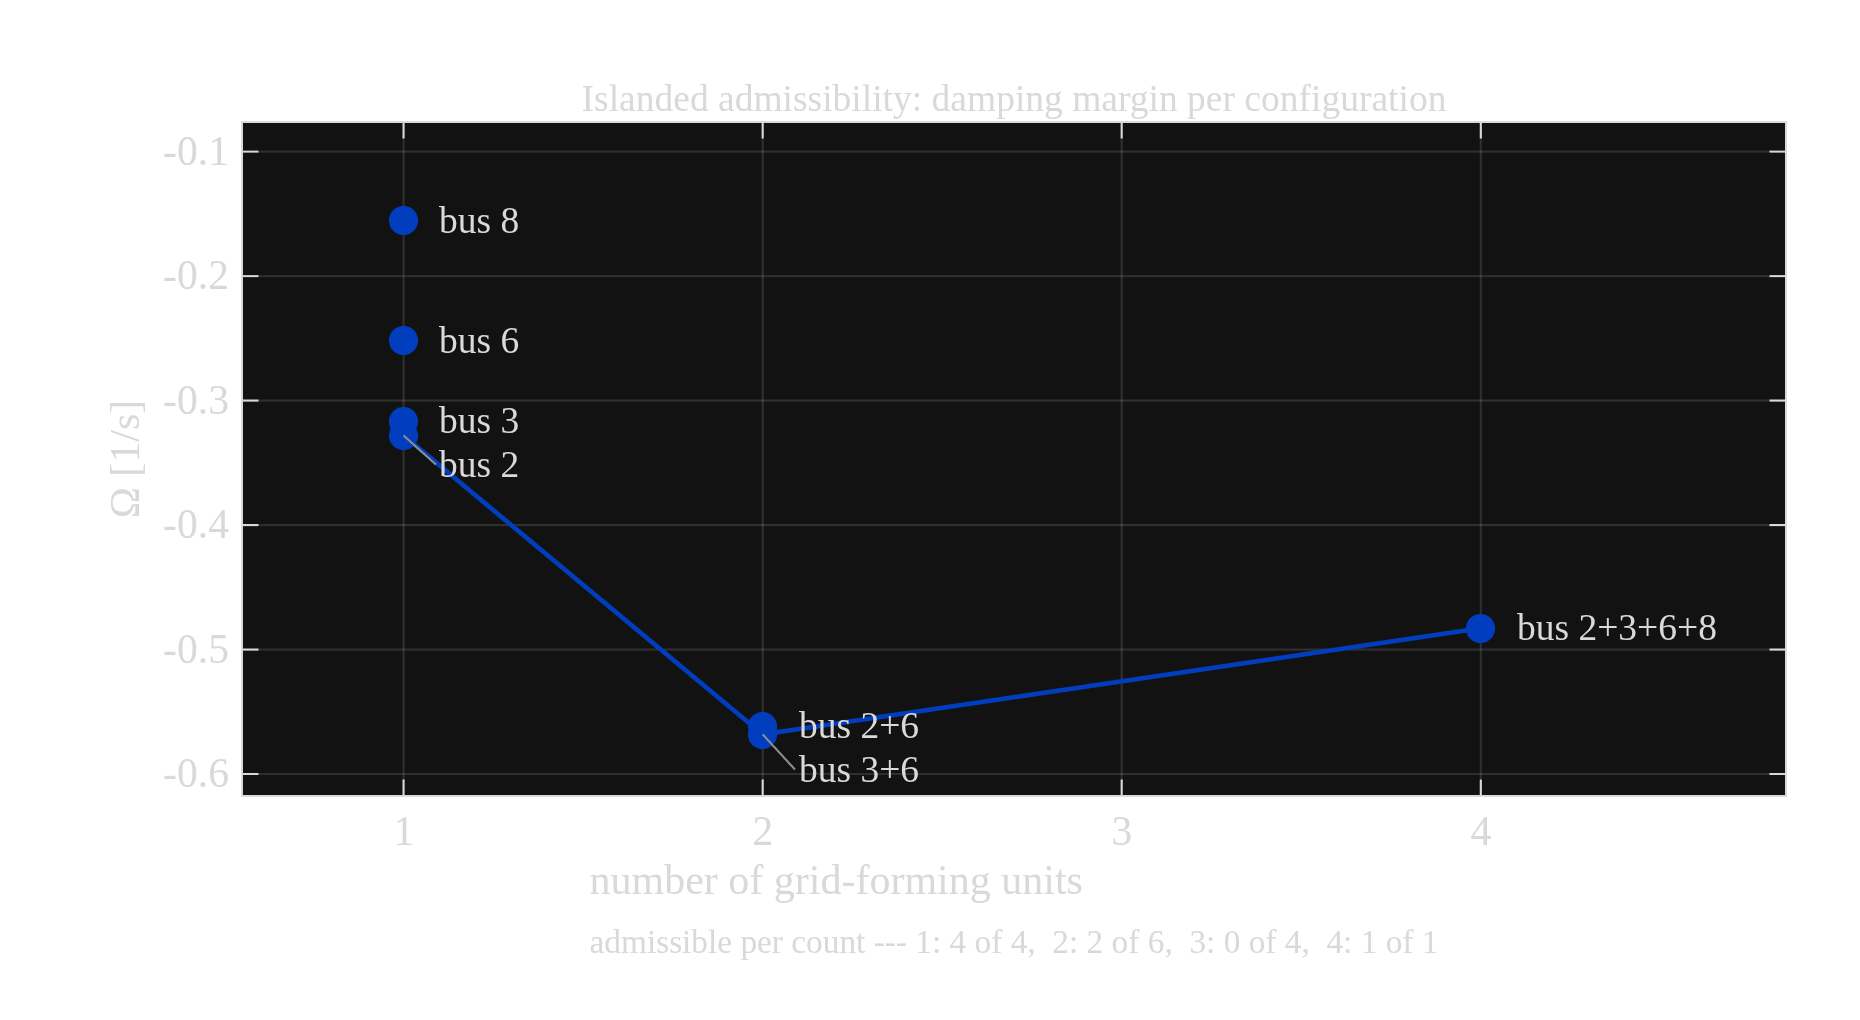
\includegraphics[width=6.20in]{figures/switch_ieee14_decision/sg_off_admissibility.png}}
 {\fbox{\parbox{6.0in}{\centering\vspace{2em}\ttfamily
   sg\_off\_admissibility.png\\[4pt]\normalfont รอการสร้างรูปใหม่.\vspace{2em}}}}
\caption{ขอบการหน่วง $\Omega$ ของทุกชุด GFM ที่รับรองได้ เทียบกับจำนวนตัว
(ค่าลบมากกว่าคือหน่วงดีกว่า) เส้นเชื่อมคือชุดที่ดีที่สุดของแต่ละจำนวน กากบาทคือชุด
ที่ไม่มีจุดสมดุล วางไว้ที่ระดับสมมติเพื่อให้เห็นตำแหน่งตามจำนวนตัวเท่านั้น
ไม่ใช่ค่า $\Omega$ ของมัน}
\label{fig:cand}
\end{figure}

\subsection{ข้อสรุปที่สาม (สำคัญที่สุด): ชุดที่ยอมรับได้ ไม่ใช่ชุดที่ไปถึงได้}
ชุดสี่ตัวผ่านการรับรองเชิงเส้นที่ $\Omega=\CandFullOmega$ แต่เมื่อ\emph{ตรึง}มันไว้
ตั้งแต่วินาทีที่ SG หลุด ระบบพังที่ $t=\ArmPinnedgfmFourHorizon\second$ ด้วย
\ArmPinnedgfmFourFailure\ รูปที่~\ref{fig:cmpwin} คอลัมน์ซ้ายแสดงกลไกตรง ๆ: ความถี่จุด
ศูนย์กลางความเฉื่อยของแขนนั้นแตกเป็นการแกว่งที่\emph{โตขึ้น}เรื่อย ๆ ขณะที่อีกสาม
แขนเข้าที่อย่างเรียบร้อย

แต่แขนสลับอัตโนมัติ\emph{ไปถึงชุดสี่ตัวเดียวกันนั้น}และรอดครบ $\NewRunEnd$ วินาที
ต่างกันที่วิธีไป: มันเลื่อนขึ้นเป็นขั้น ($\NewRunNAugment$ ครั้ง ที่
$\NewRunAugmentOne$, $\NewRunAugmentTwo$, $\NewRunAugmentThree$ และ
$\NewRunAugmentFour\second$) โดยแต่ละขั้นผ่านใบรับรองการเปลี่ยนสภาพก่อน ไม่ใช่
กระโดดไปทีเดียว

ข้อความที่ได้จึงเป็นข้อความเชิงออกแบบ ไม่ใช่เพียงตัวเลขที่ดีขึ้น:
\begin{quote}
การวิเคราะห์สัญญาณขนาดเล็กบอกว่า\emph{ปลายทาง}เสถียรหรือไม่ แต่ไม่บอกว่า
\emph{เดินไปถึงได้}หรือไม่ กลไกสลับโหมดที่มีใบรับรองรายขั้นคือสิ่งที่ปิดช่องว่างนี้
ดังนั้นการ ``เลือกชุดที่ดีที่สุดแล้วตรึงไว้'' จึงไม่เพียงพอ
\end{quote}

\subsection{ข้อสรุปที่สี่: ประโยชน์เชิงปริมาณอยู่ที่ค่าที่นิ่งแล้ว ไม่ใช่ค่ายอด}
ตารางที่~\ref{tab:excursion} เทียบสามแขนที่รอดครบขอบฟ้า ค่ายอดของการเบี่ยงเบนความถี่
ต่างกันไม่มาก แต่ค่าที่\emph{นิ่งแล้ว}ต่างกันเป็นเท่าตัว และเรียงตามจำนวน GFM ที่
ทำงานจริงอย่างเป็นระบบ

\begin{table}[H]
\centering\footnotesize
\caption{การเบี่ยงเบนความถี่ในหน้าต่าง 15 วินาทีหลังแต่ละเหตุการณ์ เฉพาะสามแขนที่
รอดครบขอบฟ้า ค่ายอดคือ $\max|f_{COI}-60|$ ค่านิ่งคือค่าเฉลี่ยของ $|f_{COI}-60|$
ใน 30\% ท้ายของหน้าต่าง หน่วยเป็นเฮิรตซ์ทั้งหมด}
\label{tab:excursion}
\begin{tabular}{lrrr|rrr}
\toprule
& \multicolumn{3}{c|}{ค่ายอด} & \multicolumn{3}{c}{ค่าที่นิ่งแล้ว} \\
เหตุการณ์ & 1 GFM & 2 GFM & สลับ & 1 GFM & 2 GFM & สลับ \\ \midrule
ตัด SG ($20\second$) &
$\DfPinnedgfmOneSGtrip$ & $\DfPinnedgfmTwoSGtrip$ & $\DfAdaptiveSGtrip$ &
$\SetPinnedgfmOneSGtrip$ & $\SetPinnedgfmTwoSGtrip$ & $\SetAdaptiveSGtrip$ \\
โหลด $+20\%$ ($50\second$) &
$\DfPinnedgfmOneLoadstep$ & $\DfPinnedgfmTwoLoadstep$ & $\DfAdaptiveLoadstep$ &
$\SetPinnedgfmOneLoadstep$ & $\SetPinnedgfmTwoLoadstep$ & $\SetAdaptiveLoadstep$ \\
ฟอลต์ ($85\second$) &
$\DfPinnedgfmOneFault$ & $\DfPinnedgfmTwoFault$ & $\DfAdaptiveFault$ &
$\SetPinnedgfmOneFault$ & $\SetPinnedgfmTwoFault$ & $\SetAdaptiveFault$ \\
เปิดสาย 6--13 ($110\second$) &
$\DfPinnedgfmOneLinetrip$ & $\DfPinnedgfmTwoLinetrip$ & $\DfAdaptiveLinetrip$ &
$\SetPinnedgfmOneLinetrip$ & $\SetPinnedgfmTwoLinetrip$ & $\SetAdaptiveLinetrip$ \\
ต่อกลับ ($145\second$) &
$\DfPinnedgfmOneRestorereclose$ & $\DfPinnedgfmTwoRestorereclose$ &
$\DfAdaptiveRestorereclose$ &
$\SetPinnedgfmOneRestorereclose$ & $\SetPinnedgfmTwoRestorereclose$ &
$\SetAdaptiveRestorereclose$ \\
\bottomrule
\end{tabular}
\end{table}

กลไกคือการแบ่งกันรับภาระตามค่า droop: เมื่อมี $n$ ตัวถือหน้าที่สร้างแรงดัน แต่ละตัว
รับความไม่สมดุลเพียงเศษหนึ่งส่วน $n$ ค่าเบี่ยงเบนที่สภาวะคงตัวร่วมจึงเล็กลงตามส่วน
ค่าที่วัดได้ในหน้าต่างโหลดเพิ่มเรียงเป็น $\SetPinnedgfmOneLoadstep$,
$\SetPinnedgfmTwoLoadstep$ และ $\SetAdaptiveLoadstep$~Hz สำหรับ 1, 2 และ (สูงสุด)
$\NewRunGfmMax$ ตัว ซึ่งเข้ากับสัดส่วน $1/n$ โดยที่ส่วนต่างที่เหลืออธิบายได้จาก
พิกัดของอุปกรณ์ที่ไม่เท่ากัน

\emph{สิ่งที่ต้องรายงานตามจริง} ที่หน้าต่างการตัด SG เอง แขนที่ตรึงไว้ทำได้
\emph{ดีกว่า} แขนสลับ ($\DfPinnedgfmOneSGtrip$ และ $\DfPinnedgfmTwoSGtrip$ เทียบ
$\DfAdaptiveSGtrip$~Hz) เพราะแขนสลับต้องจ่ายค่าชั่วครู่ของลำดับการเลื่อนขึ้นของตัวเอง
ผลนี้ถูกรายงานตามที่วัดได้ ไม่ถูกตัดออก

\clearpage
\begin{figure}[H]
\centering
\IfFileExists{figures/switch_ieee14_decision/comparison_full.png}
 {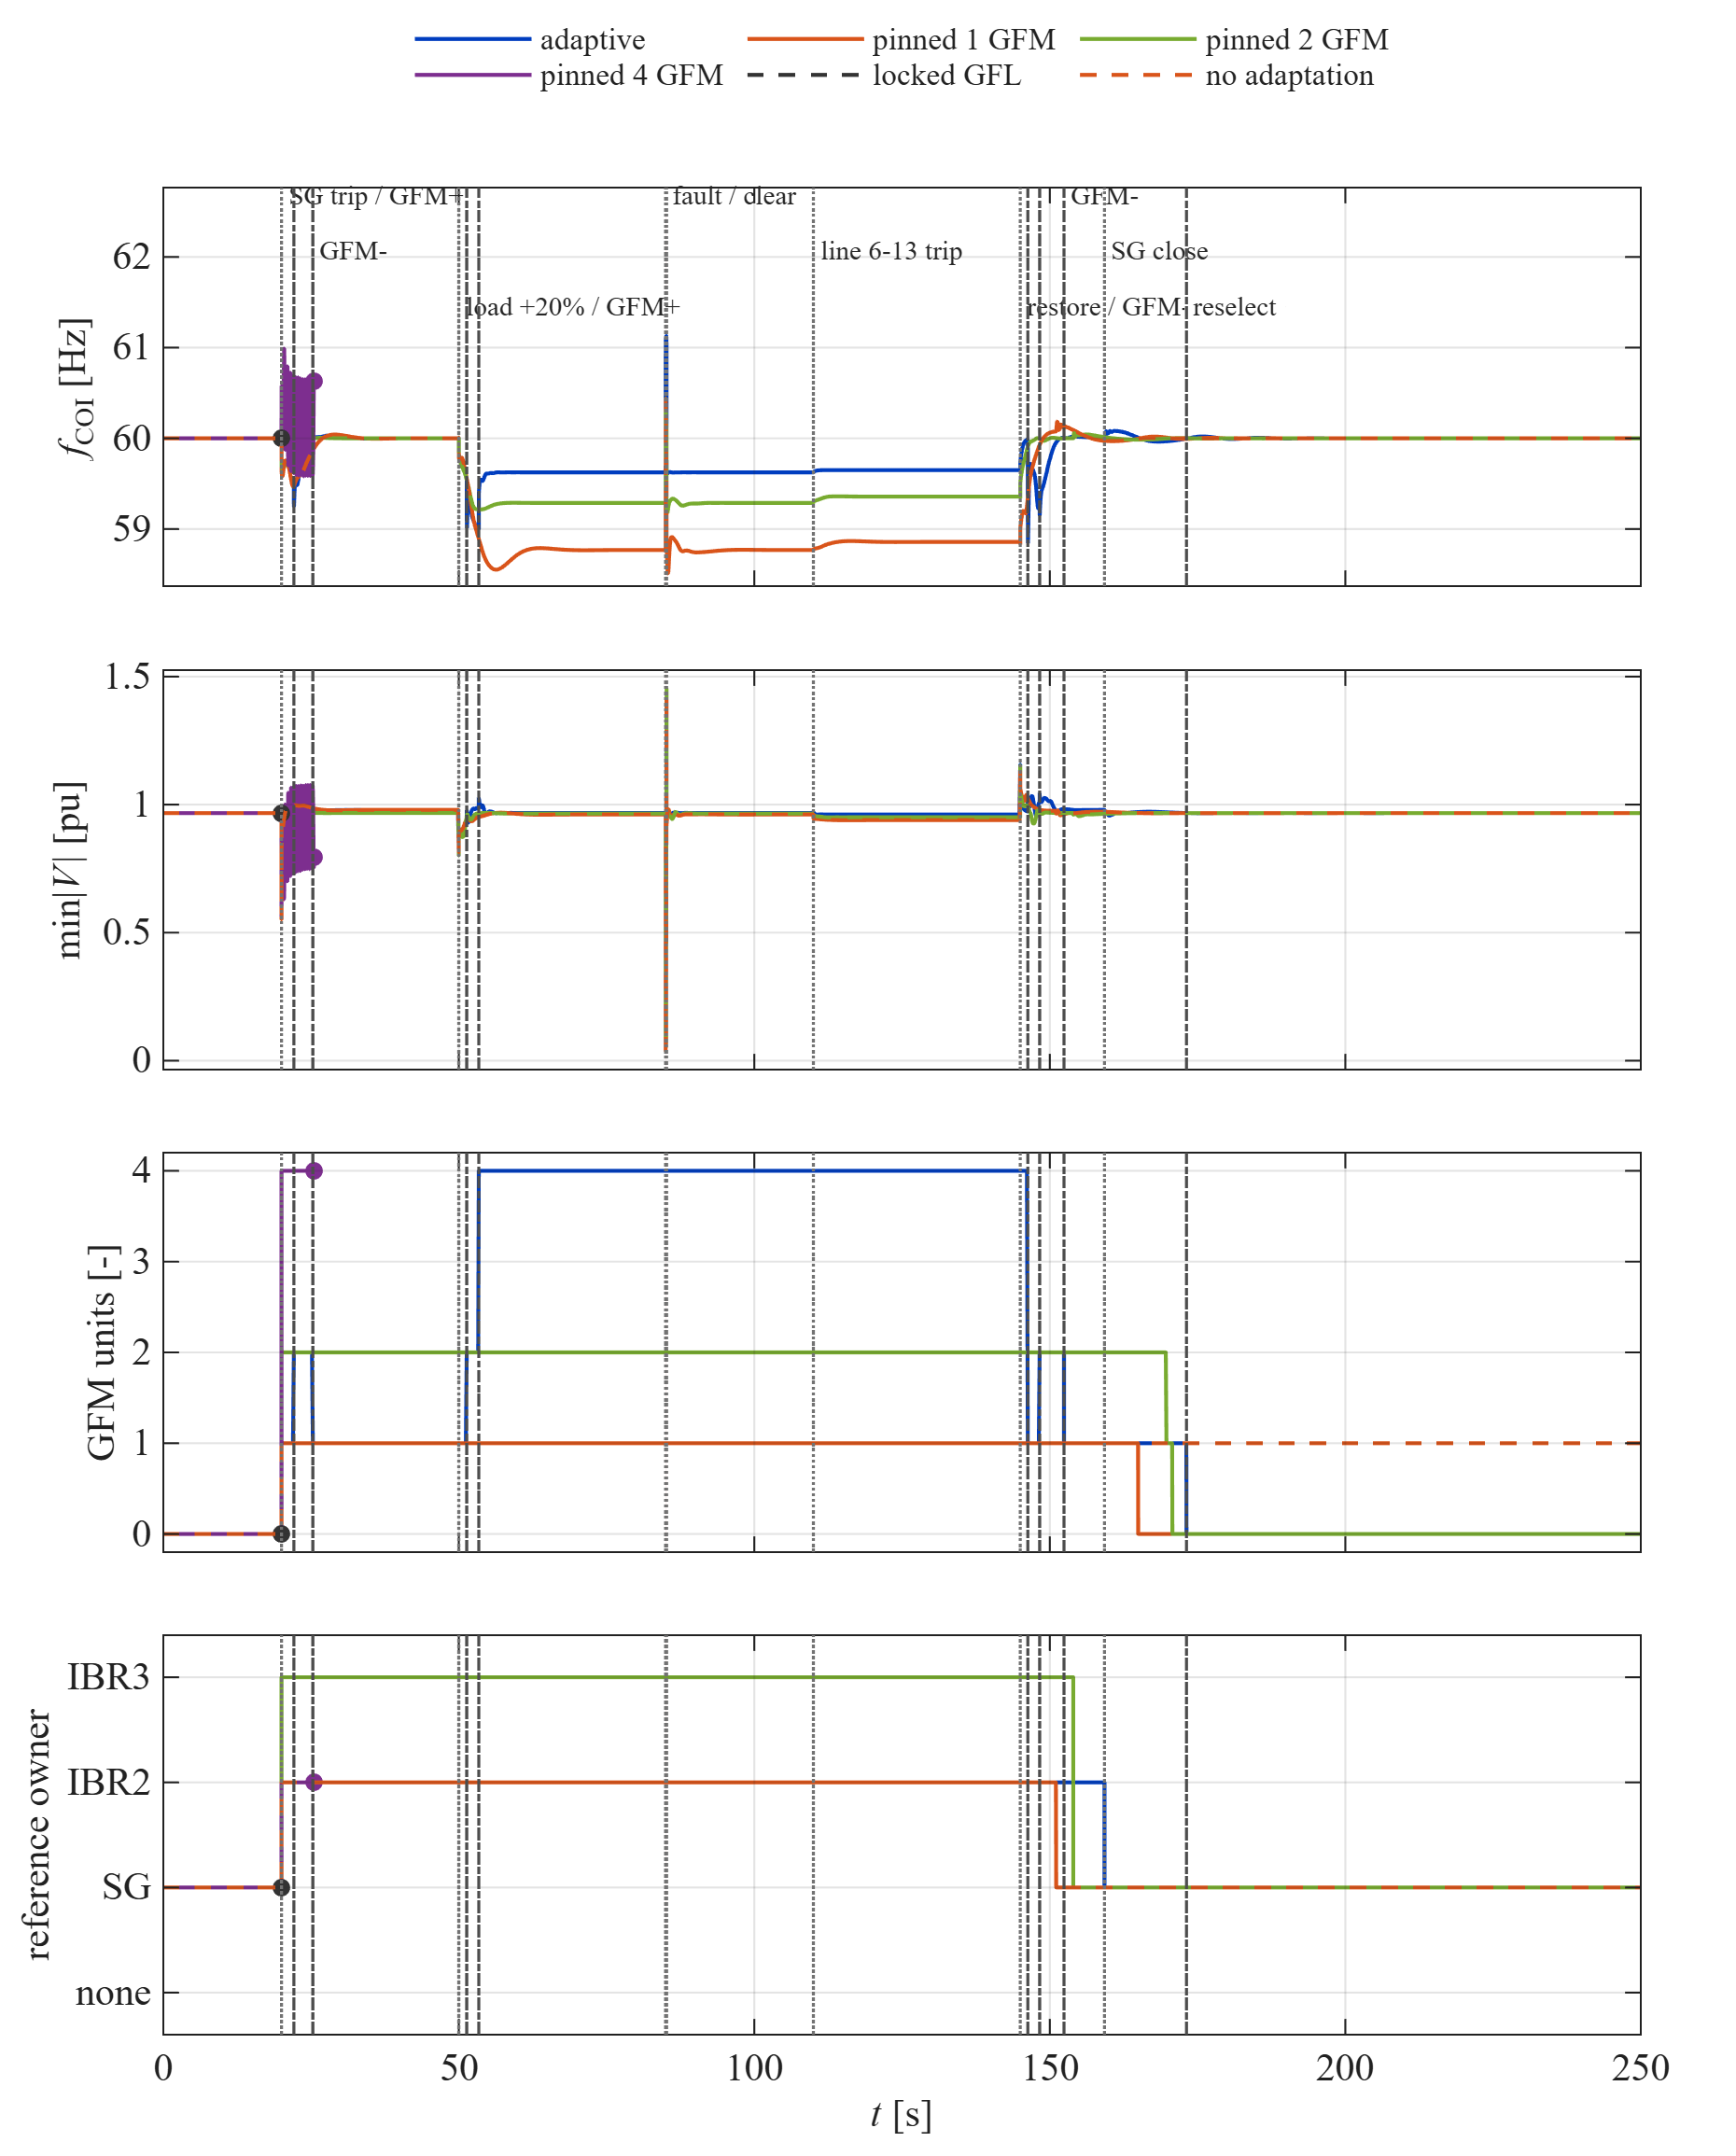
\includegraphics[width=6.20in]{figures/switch_ieee14_decision/comparison_full.png}}
 {\fbox{\parbox{6.0in}{\centering\vspace{2em}\ttfamily comparison\_full.png\\[4pt]
   \normalfont รอการสร้างรูปใหม่.\vspace{2em}}}}
\caption{ห้าแขนวางทับกันบนขอบฟ้าเต็ม แถวจากบนลงล่าง: ความถี่จุดศูนย์กลางความเฉื่อย
แรงดันต่ำสุดของเครือข่าย จำนวนหน่วยที่สร้างแรงดัน และเจ้าของมุมอ้างอิง ลำดับเหตุการณ์
ถูกระบุเพียงครั้งเดียวบนแถวบนสุดในแถบที่กันไว้เหนือข้อมูล หน้านี้อ่านพฤติกรรม
\emph{ที่เข้าที่แล้ว}: สามแขนที่รอดแยกออกเป็นสามระดับความถี่ที่ชัดเจน และการเลื่อน
ขึ้นเป็นขั้น $1\!\to\!2\!\to\!4$ ของแขนสลับเห็นได้ในแถวที่สาม แขนที่จบก่อนขอบฟ้าหยุด
ที่จุดตัวอย่างสุดท้ายของตัวเอง (จุดทึบ) และ\emph{ไม่}ถูกต่อเติม ตรึงค่า หรือประมาณค่า
นอกช่วงให้ยาวเท่าแขนอื่น ช่วงแกนตั้งทุกแผงมาจากข้อมูลที่อยู่ในหน้าต่างเวลาที่วาดจริง
และตัวสร้างรูปจะหยุดถ้ามีจุดใดหลุดออกนอกช่วงนั้น}
\label{fig:cmparms}
\end{figure}

\clearpage
\begin{figure}[H]
\centering
\IfFileExists{figures/switch_ieee14_decision/comparison_windows.png}
 {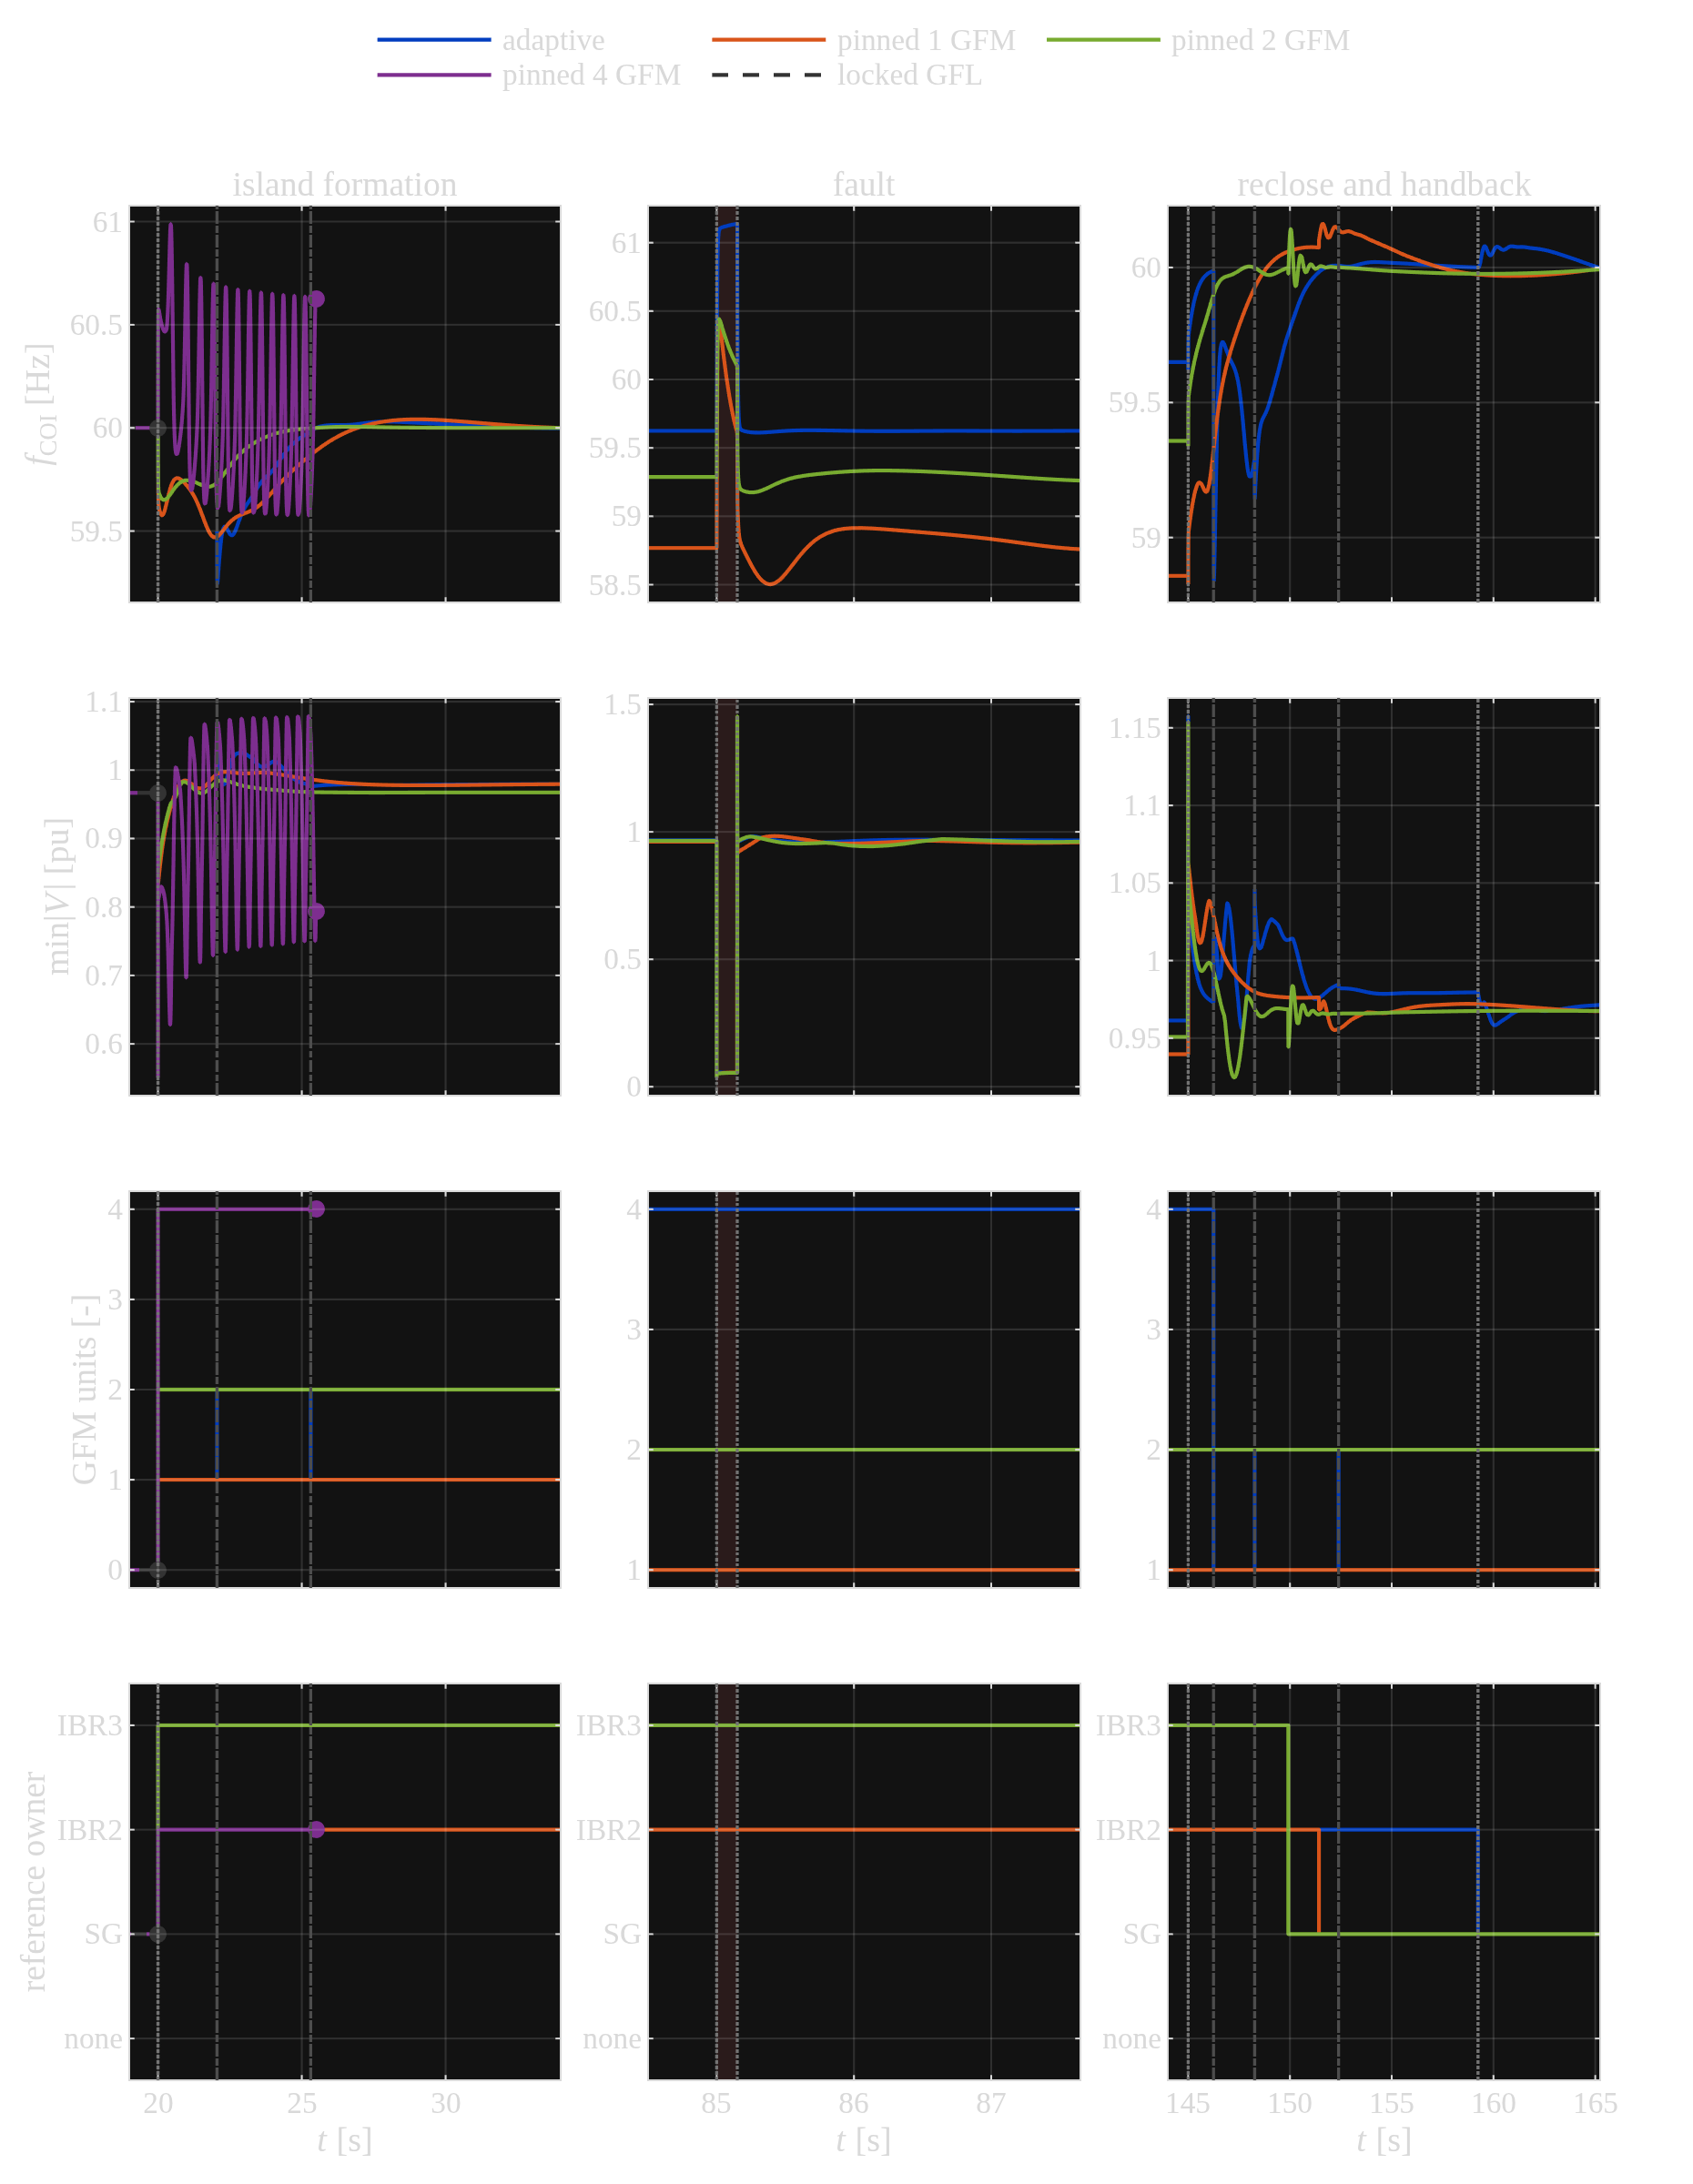
\includegraphics[width=6.20in]{figures/switch_ieee14_decision/comparison_windows.png}}
 {\fbox{\parbox{6.0in}{\centering\vspace{2em}\ttfamily comparison\_windows.png\\[4pt]
   \normalfont รอการสร้างรูปใหม่.\vspace{2em}}}}
\caption{สี่แถวเดียวกันบนสามหน้าต่างที่ค่าชั่วครู่แยกแยะได้ ขอบเขตทุกหน้าต่างมาจาก
ตารางเหตุการณ์ ซ้าย: การสร้างเกาะ ซึ่งแขนที่ตรึงสี่ตัวแตกเป็นการแกว่งที่โตขึ้นแล้ว
ยุติลง กลาง: ฟอลต์ โดยแรเงาช่วงชันต์ $0.150$~s แสดงแรงดันต่ำสุดของเครือข่ายที่ทรุด
ลงแล้วฟื้นขึ้น ขวา: การต่อกลับและการส่งคืนหน้าที่ แต่ละคอลัมน์ปรับสเกลตามหน้าต่าง
ของตัวเอง ซึ่งเป็นสิ่งที่รูปหน้าเดียวฉบับก่อนทำไม่ได้}
\label{fig:cmpwin}
\end{figure}

\begin{figure}[H]
\centering
\IfFileExists{figures/switch_ieee14_decision/comparison_event_excursions.png}
 {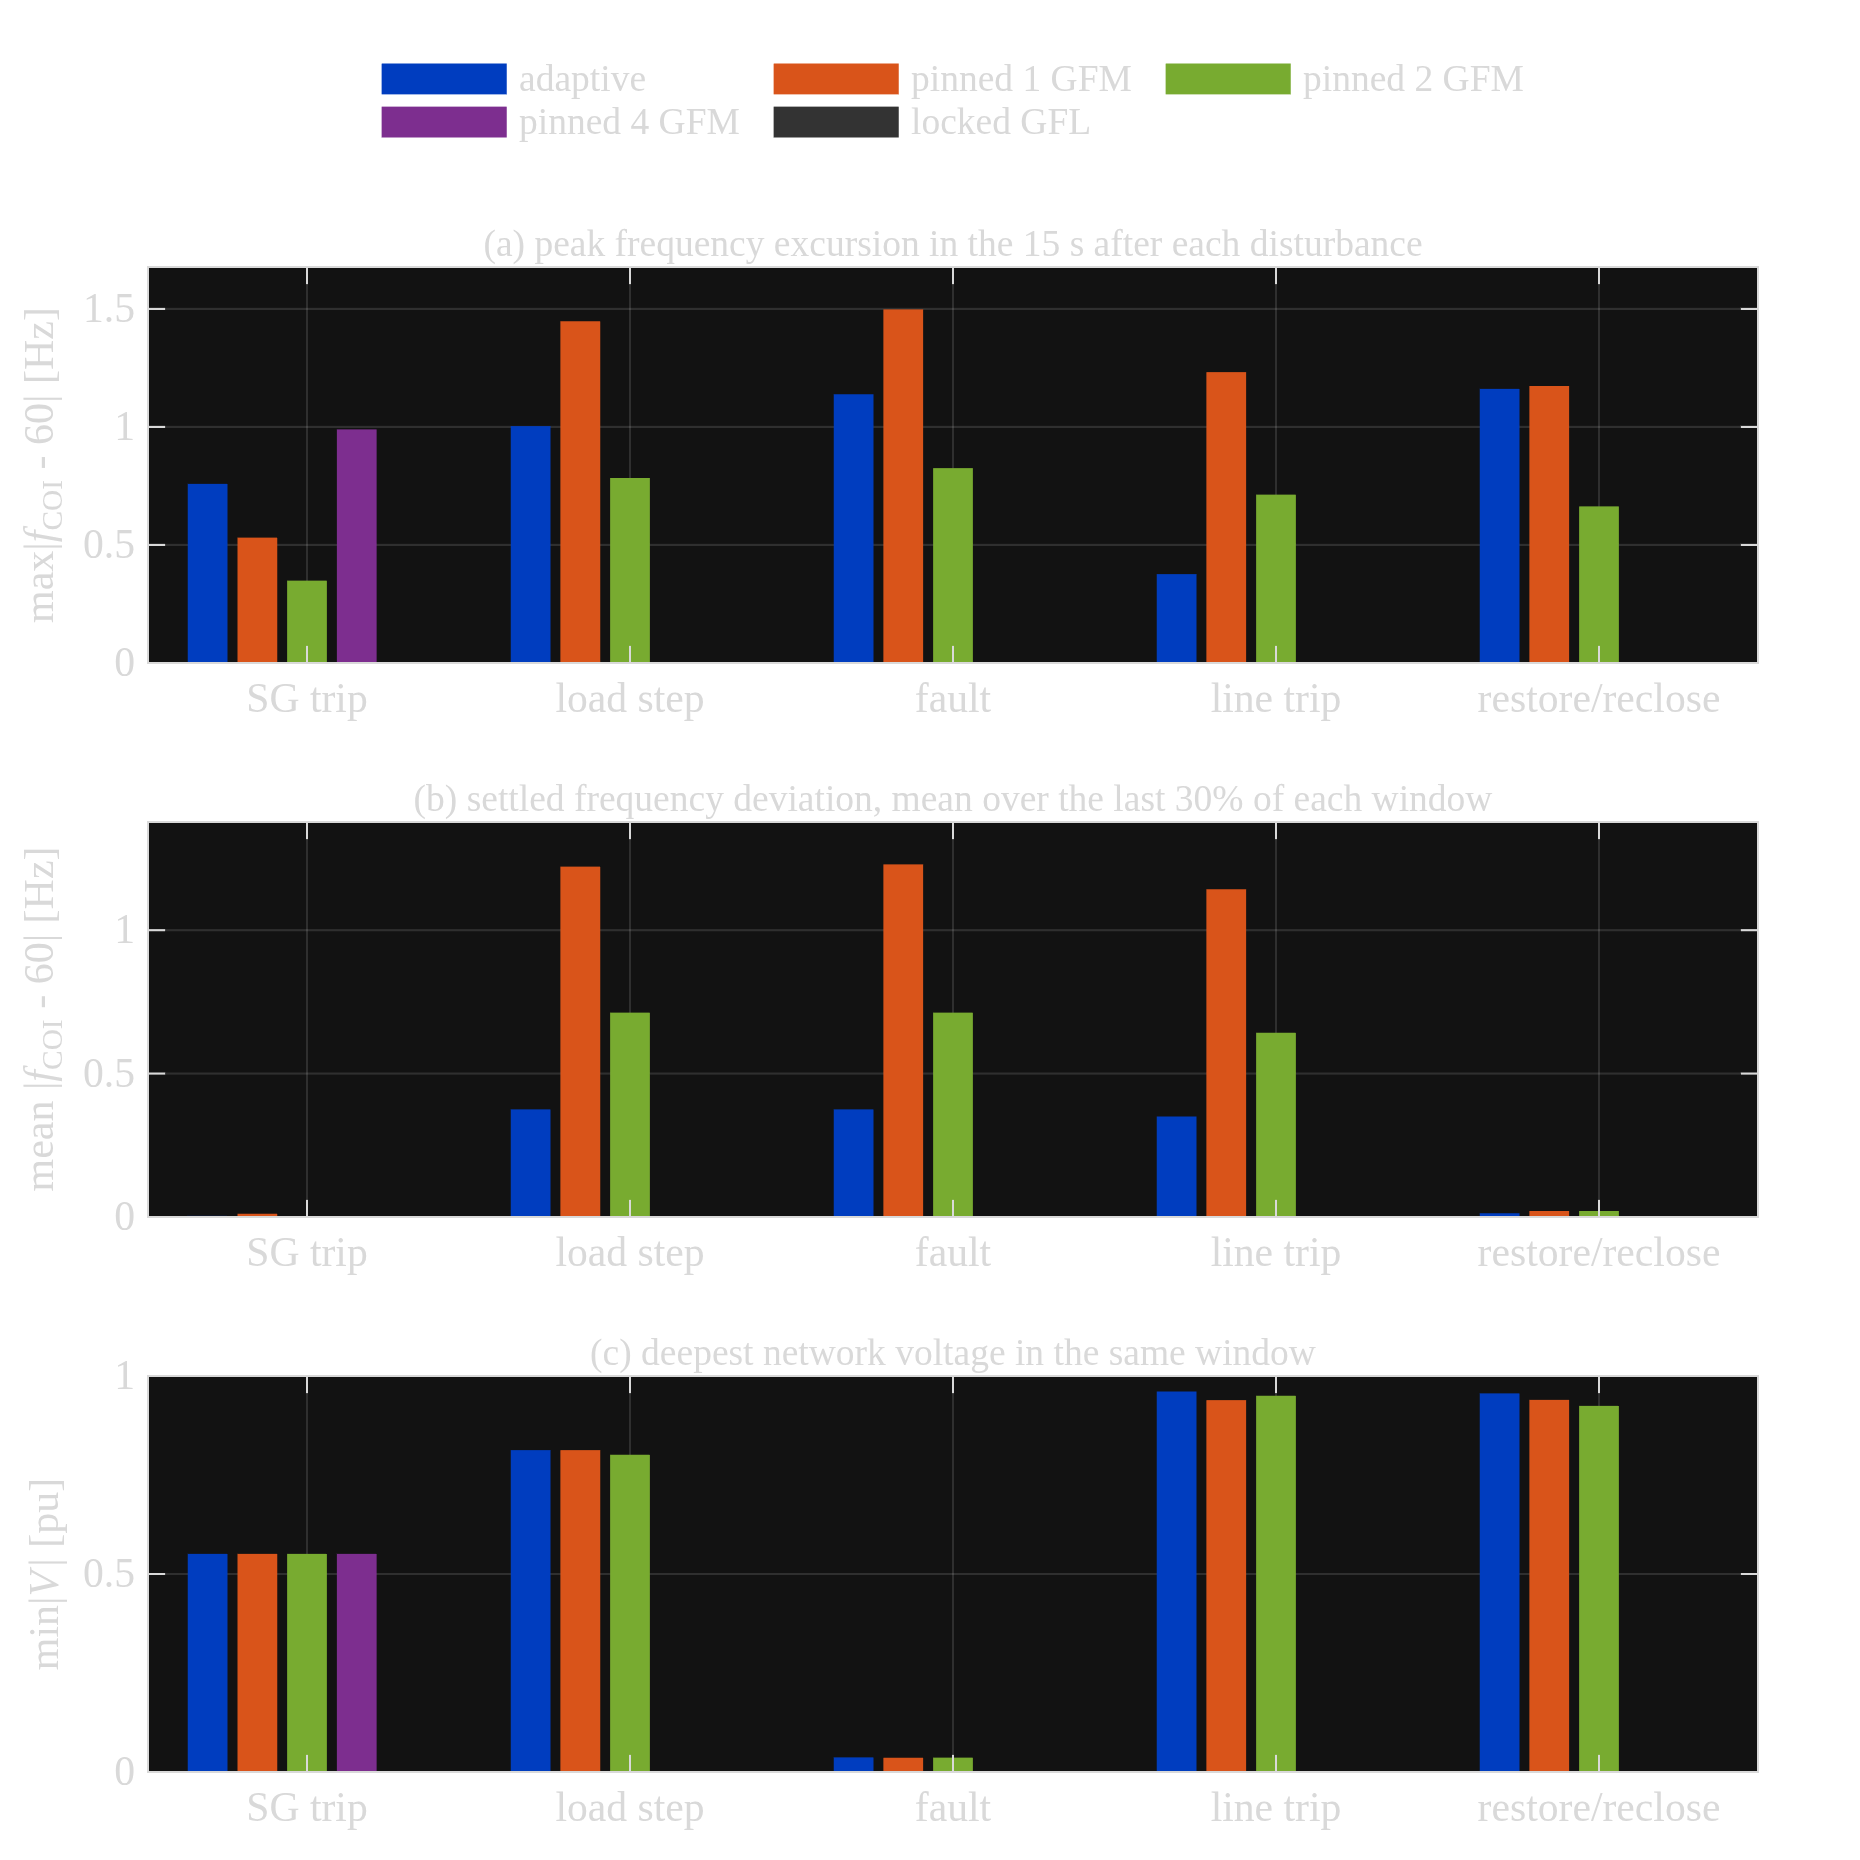
\includegraphics[width=6.20in]{figures/switch_ieee14_decision/comparison_event_excursions.png}}
 {\fbox{\parbox{6.0in}{\centering\vspace{2em}\ttfamily
   comparison\_event\_excursions.png\\[4pt]\normalfont
   รอการสร้างรูปใหม่.\vspace{2em}}}}
\caption{(a) ค่ายอดของการเบี่ยงเบนความถี่ในหน้าต่าง 15 วินาทีหลังแต่ละเหตุการณ์
(b) ค่าที่นิ่งแล้วในหน้าต่างเดียวกัน (c) แรงดันต่ำสุดของเครือข่าย
แท่งที่หายไปหมายถึงแขนนั้นไม่ได้เดินเข้าไปในหน้าต่างนั้น ไม่ใช่ค่าศูนย์}
\label{fig:cmpbars}
\end{figure}

\subsection{กรณีระบบที่มี SG ห้าเครื่อง: ยังทำไม่ได้ และนี่คือเหตุผล}\label{sec:fivesg}
การเทียบที่สมบูรณ์ควรมีแขนที่สี่: ระบบ IEEE-14 แบบเดิมที่ทุกหน่วยผลิตเป็นเครื่อง
ซิงโครนัสห้าเครื่อง แล้วตัดออกหนึ่งเครื่อง รายงานฉบับนี้\textbf{ไม่มี}แขนนั้น และ
ไม่เติมตัวเลขสมมติแทน เหตุผลมีสองชั้นและตรวจสอบได้ทั้งคู่

\emph{ชั้นข้อมูล} ที่เก็บในรีโปมีข้อมูลไดนามิกรายเครื่อง (ค่ารีแอกแตนซ์ ค่าคงเวลา
ความเฉื่อย) ของเครื่องที่บัส 1 เพียงเครื่องเดียว สำหรับบัส 2, 3, 6 และ 8 ไม่มีชุด
ค่าที่ผ่านการตรวจแหล่งอ้างอิง การสร้างแขนนั้นจึงต้องนำค่าจากที่อื่นเข้ามา ซึ่งเป็น
การตัดสินใจเรื่องแหล่งข้อมูลที่ต้องบันทึกแยกก่อน ไม่ใช่ผลพลอยได้ของงานรายงาน

\emph{ชั้นเครื่องมือ} เส้นทางไฮบริดที่ใช้อยู่รองรับเครื่องซิงโครนัสเพียงเครื่องเดียว
โดยโครงสร้าง มีจุดที่ปฏิเสธแบบ fail-closed อย่างน้อยสี่จุดอิสระกัน: ตัวสร้างอุปกรณ์
SG, ตัวเลือกชุดที่ต้องมีเจ้าของอ้างอิงซิงโครนัสหนึ่งเดียว, ตัวแก้จุดสมดุลผสมที่
ต้องการ SG หนึ่งตัวที่บัสอ้างอิงของเคส และตัวควบคุมการซิงโครไนซ์ตอนต่อกลับ การเปิด
ทางให้ห้าเครื่องจึงเป็นการขยายขอบเขตของ kernel ไม่ใช่การเปลี่ยนค่าตัวเลือก

ถึงกระนั้น ข้อเท็จจริงเชิงกายภาพที่เกี่ยวข้องที่สุดยังพูดได้จากข้อมูลที่มี: ในเคสนี้
เครื่องซิงโครนัสมีเพียงเครื่องเดียว ดังนั้นเมื่อมันหลุด ความเฉื่อยซิงโครนัสของเกาะ
ไฟฟ้าเป็น\emph{ศูนย์} ต่างจากระบบห้าเครื่องที่ตัดออกหนึ่งเครื่องซึ่งยังเหลืออีกสี่
เครื่องช่วยรับ นั่นคือเหตุที่กรณีนี้ยากกว่าโดยธรรมชาติ และเป็นเหตุผลที่การมีอุปกรณ์
สร้างแรงดันจากอินเวอร์เตอร์เป็นเรื่องจำเป็น ไม่ใช่ทางเลือกเพื่อความสวยงาม

%=============================================================================
\section{ข้อจำกัด}\label{sec:lim}
%=============================================================================
\begin{itemize}\itemsep2pt
  \item \textbf{ไม่มีข้ออ้างเรื่องความพร้อมใช้งานเชิงปฏิบัติการ} การที่วิถี
        $\NewRunEnd$ วินาทีเป็นคำตอบที่ลู่เข้าและถูกยอมรับของระบบ DAE รวม
        บอกได้เพียงว่าการคำนวณสอดคล้องกันในตัวเอง ไม่ใช่หลักฐานของการผ่านเกณฑ์
        กริดโค้ด การประสานงานของระบบป้องกัน หรือความเป็นไปได้ในการสร้างฮาร์ดแวร์
  \item \textbf{ค่าสุดขีดชั่วครู่คือค่าสุดขีด ไม่ใช่พิกัดใช้งาน} วิถีที่ยอมรับมี
        แรงดันเครือข่ายขึ้นถึงจุดสูงสุด $\NewRunVMax\pu$ และความถี่จุดศูนย์กลางความ
        เฉื่อยอยู่ในแถบ $\NewRunFMin$--$\NewRunFMax$~Hz ระหว่างช่วงฟอลต์และช่วงสลับ
        โหมด ค่าเหล่านี้เป็นการแกว่งจริงของแบบจำลองภายใต้ลำดับเหตุการณ์ที่รุนแรง ซึ่ง
        ถูกเปิดเผยตรง ๆ ไม่ใช่ค่าที่สภาวะคงตัว และย้ำว่างานนี้เป็นการศึกษาเชิงตัวเลข
        ไม่ใช่การลงนามรับรองการออกแบบ
  \item \textbf{การวิเคราะห์เชิงเส้นเพียงจุดเดียว} สเปกตรัมในหัวข้อ~\ref{sec:sssa}
        และค่า $\Omega$ ในตารางการรับรองเป็นการวิเคราะห์ที่จุดทำงานจุดเดียวต่อชุด
        จึงไม่ให้ขอบเขตแก่ระบบแบบสลับโหมด หัวข้อ~\ref{sec:compare} แสดงกรณีที่ชุด
        ผ่านการรับรองแล้วยังไปถึงไม่ได้ ซึ่งเป็นข้อจำกัดของเครื่องมือเชิงเส้นเอง
  \item \textbf{ดัชนีอ้างอิงเป็นเชิงวินิจฉัยเท่านั้น} เฉพาะ $S$, $J_V$ และ $J_f$
        ที่เข้าการตัดสินใจ ส่วน $J_R$, $J_P$, $J_{\mathrm{lock}}$ และ
        $J_{\mathrm{SCR}}$ ในรูปที่~\ref{fig:agsi} คำนวณหลังวิถีเสร็จ ไม่เข้าเกตใด
        จัดชั้น \textsf{ASSUMED\_DIAGNOSTIC} และห้ามใช้สนับสนุนข้ออ้างความพร้อมใช้งาน
        ไม่มีการรวมดัชนีเหล่านี้เป็นดัชนีเดียวโดยเจตนา เพราะดัชนีรวมอยู่ห่างจากการ
        เป็นตัวแปรตัดสินใจเพียงก้าวเดียว
  \item \textbf{ขอบเขตของการเปรียบเทียบ} หัวข้อ~\ref{sec:compare} เทียบ
        ``สลับเทียบไม่สลับ'' บนสัดส่วนทรัพยากรนี้เท่านั้น ไม่ได้เทียบตัวเลือกชุดนี้
        กับตัวเลือกชุดอื่น ไม่ได้อ้างอะไรกับระบบที่มีแหล่งสร้างแรงดันอื่น และไม่ได้
        อ้างความเหนือกว่าเชิงตัวเลข (เรซิดวลและจำนวนขั้นที่ปฏิเสธเทียบข้ามแขนที่ยาว
        ไม่เท่ากันไม่ได้) แขนที่จบก่อนขอบฟ้าไม่ถูกต่อเติมให้ยาวเท่าแขนอื่น
  \item \textbf{ไม่มีแขน SG ห้าเครื่อง} ตามที่อธิบายไว้ในหัวข้อ~\ref{sec:fivesg}
        รีโปมีข้อมูลไดนามิกรายเครื่องของบัส 1 เท่านั้น และเส้นทางไฮบริดปฏิเสธหลาย
        เครื่องแบบ fail-closed อยู่สี่จุด จึงไม่มีตัวเลขของแขนนั้นในรายงานนี้ และ
        ไม่มีการเติมค่าสมมติแทน
\end{itemize}

\end{document}
